\documentclass[11pt, a4paper]{report}
%\documentclass[11pt, a4paper]{article}

%====================== PACKAGES ======================


\usepackage[french]{babel}

\frenchbsetup{StandardLists=true}
\usepackage{enumitem}
\usepackage{pifont}

\usepackage[utf8x]{inputenc}
%\usepackage[latin1]{inputenc} % Feynman

%pour gérer les positionnement d'images
\usepackage{float}
\usepackage{amsmath}
\DeclareMathOperator{\dt}{dt}
\usepackage{graphicx}
\usepackage{tabularx}
\usepackage[colorinlistoftodos]{todonotes}
\usepackage{url}
%pour les informations sur un document compilé en PDF et les liens externes / internes
\usepackage[pdfborder=0]{hyperref}
\hypersetup{
	colorlinks = true
	}
%pour la mise en page des tableaux
\usepackage{array}
\usepackage{tabularx}
\usepackage{multirow}
\usepackage{multicol}
\setlength{\columnsep}{50pt}
%pour utiliser \floatbarrier
%\usepackage{placeins}
%\usepackage{floatrow}
%espacement entre les lignes
\usepackage{setspace}
%modifier la mise en page de l'abstract
\usepackage{abstract}
%police et mise en page (marges) du document
\usepackage[T1]{fontenc}
\usepackage[top=2cm, bottom=2cm, left=2cm, right=2cm]{geometry}
%Pour les galerie d'images
\usepackage{subfig}

\usepackage{pdfpages}
\usepackage{tikz}
%\usepackage{tikz}
\usetikzlibrary{trees}
\usetikzlibrary{decorations.pathmorphing}
\usetikzlibrary{decorations.markings}
\usetikzlibrary{decorations.pathreplacing,calligraphy}
\usetikzlibrary{decorations.pathmorphing,calc,shapes,shapes.geometric,patterns}
%\usetikzlibrary{decorations}
\usetikzlibrary{angles, quotes}
\usepackage{verbatim}

\usepackage{appendix}

\usepackage{comment}

\usepackage{xcolor}

\hypersetup{colorlinks=true,linkcolor=black}

\usepackage{makeidx}

%\PreviewEnvironment{tikzpicture}
%\setlength\PreviewBorder{0pt}%

%====================== INFORMATION ET REGLES ======================

%rajouter les numérotation pour les \paragraphe et \subparagraphe
\setcounter{secnumdepth}{4}
\setcounter{tocdepth}{4}

\hypersetup{							% Information sur le document
pdfauthor = {Stephan Runigo},			% Auteurs
pdftitle = {Documentation},			% Titre du document
pdfsubject = {Documentation},		% Sujet
pdfkeywords = {Document},	% Mots-clefs
pdfstartview={FitH}}	% ajuste la page à la largeur de l'écran
%pdfcreator = {MikTeX},% Logiciel qui a crée le document
%pdfproducer = {} % Société avec produit le logiciel
\makeindex % Créer un index
%======================== DEBUT DU DOCUMENT ========================
%
\begin{document}
%
%régler l'espacement entre les lignes
\newcommand{\HRule}{\rule{\linewidth}{0.5mm}}
%
% Titre, résumé, ... %
%
\begin{titlepage}
%
~\\[1cm]

\begin{center}
%\includegraphics[scale=0.5]{./presentation/chambreABulle}
\end{center}

\textsc{\Large }\\[0.5cm]

% Title \\[0.4cm]
\HRule

\begin{center}
{\huge \bfseries  La causalité\\
%titre 2\\[0.4cm]
 }
\end{center}

\HRule \\[1.5cm]

\begin{center}
%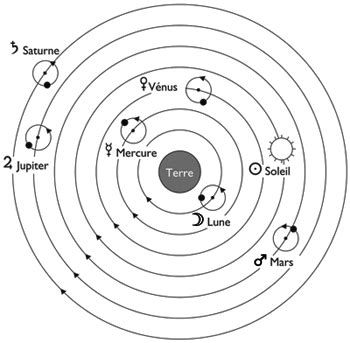
\includegraphics[scale=0.3]{./presentation/ptoleme}
\end{center}

\begin{center}
%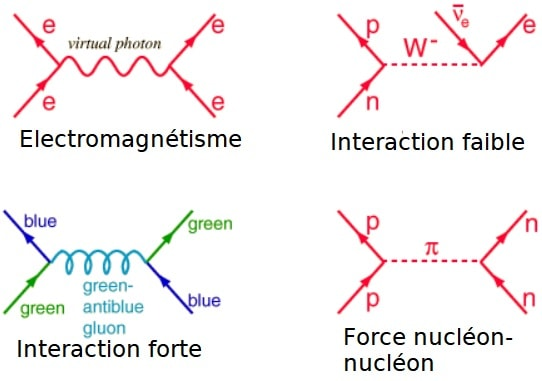
\includegraphics[scale=0.3]{./presentation/diagrammesInteractions}
\end{center}


% Author and supervisor
\begin{minipage}{0.4\textwidth}
\begin{flushleft} \large
%\emph{Auteur:}\\
%Stephan \textsc{Runigo}
\end{flushleft}
\end{minipage}
\begin{minipage}{0.4\textwidth}
\begin{flushright} \large
\emph{Auteur:}\\
Stephan \textsc{Runigo}
\end{flushright}
\end{minipage}

\vfill

% Bottom of the page
{\large \today}

\end{titlepage}

\newpage
\begin{center}
\Large
Résumé
\normalsize
\end{center}
\vspace{3cm}
\begin{itemize}[leftmargin=1cm, label=\ding{32}, itemsep=21pt]
\item {\bf Objet : } Souvenir des questions posés.
\item {\bf Contenu : } Définition, analyse, reflexion.
\item {\bf Public concerné : } Interressé à la question de l'âme.
\end{itemize}

\vspace{3cm}



\vspace{3cm}


%

%
% Table des matières
\tableofcontents
\thispagestyle{empty}
\setcounter{page}{0}
%
%espacement entre les lignes des tableaux
\renewcommand{\arraystretch}{1.5}
%
%====================== INCLUSION DES PARTIES ======================
%
~
\thispagestyle{empty}
%recommencer la numérotation des pages à "1"
\setcounter{page}{0}
\newpage
%
%%
\chapter{Cosmologie}
%

%%%%%%%%%%%%%%%%%%%%%%%%%%%%%%%%%%%%%%%%%%%%
\section{Les cosmologies antiques}

%%%%%%%%%%%%%%%%%%%%%%%%%%%%%%%%%%%%%%%%%%%%

  \subsection{Première cosmologie}

\begin{center}

\begin{tikzpicture}
    \def\horizontal {0.35}
    \def\vertical {1.3}
\begin{scope}
\draw[-latex,color=darkgray] (-37*\horizontal,0) -- (5*\horizontal,0);
\draw[shift={(5*\horizontal,0)},color=darkgray,thin]
                                   node[below] {\footnotesize $temps$};
%3500 av JC
  \draw[shift={(-35*\horizontal,0)},color=darkgray,thin] (0pt,1pt) -- (0pt,-1pt)
                                   node[above,text width=3cm,text centered]{ Invention de l'écriture en mésopotamie}
                                   node[below] {\footnotesize -3500 ans};
%776 av JC
  \draw[shift={(-12*\horizontal,0)},color=darkgray,thin] (0pt,1pt) -- (0pt,-1pt)
                                   node[above,text width=3cm,text centered]{ Invention de l'alphabet par les phéniciens}
                                   node[below] {\footnotesize -1200 ans};
  \draw[shift={(0,0)},color=darkgray,thin] (0pt,1pt) -- (0pt,-1pt)
                                   node[below] {\footnotesize 0}
                                   node[above,text width=3cm,text centered]{ Naissance de Jésus Christ};
%\draw (1.4*\horizontal,0.5*\vertical) node [rotate=30]{Ptolémé};
\end{scope}
\begin{scope}[yshift= -1.5cm]
    \def\vertical {0.3}
  \shade[bottom color=brown!10!gray!10!green, top color=white,shading angle={90},rounded corners=1pt]
 (-37*\horizontal,0) rectangle (-35*\horizontal, \vertical);
  \shade[bottom color=brown!10!gray!10!green, top color=brown!10!gray!10!green,shading angle={90},rounded corners=1pt]
 (-35*\horizontal,0) rectangle (-5*\horizontal, \vertical);
  \shade[bottom color=white, top color=brown!10!gray!10!green,shading angle={90},rounded corners=1pt]
 (-5*\horizontal,0) rectangle (-3*\horizontal, \vertical);
  \node[above] (P) at (-20*\horizontal,\vertical) {Civilisation summérienne}; % SUMÉRIENS

    \def\decalage {-1}
  \shade[bottom color=brown!10!gray!10!green, top color=white,shading angle={90},rounded corners=1pt]
 (-28*\horizontal, \decalage) rectangle (-25*\horizontal, \vertical + \decalage);
  \shade[bottom color=brown!10!gray!10!green, top color=brown!10!gray!10!green,shading angle={90},rounded corners=1pt]
 (-25*\horizontal, \decalage) rectangle (-2*\horizontal, \vertical + \decalage);
  \shade[bottom color=white, top color=brown!10!gray!10!green,shading angle={90},rounded corners=1pt]
 (-2*\horizontal, \decalage) rectangle (0*\horizontal, \vertical + \decalage);
  \node[above] (P) at (-15*\horizontal,\vertical  + \decalage) {Civilisation égyptienne}; % ÉGYPTIENS

    \def\decalage {-2}
  \shade[bottom color=brown!10!gray!10!green, top color=white,shading angle={90},rounded corners=1pt]
 (-10*\horizontal, \decalage) rectangle (-8*\horizontal, \vertical + \decalage);
  \shade[bottom color=brown!10!gray!10!green, top color=brown!10!gray!10!green,shading angle={90},rounded corners=1pt]
 (-8*\horizontal, \decalage) rectangle (1*\horizontal, \vertical + \decalage);
  \shade[bottom color=white, top color=brown!10!gray!10!green,shading angle={90},rounded corners=1pt]
 (1*\horizontal, \decalage) rectangle (3*\horizontal, \vertical + \decalage);
  \node[above] (P) at (-4*\horizontal,\vertical  + \decalage) {Civilisation grec}; % CRECS
\end{scope}
\end{tikzpicture}


%%%%%%%%%%%%%%%%%%%%%%%%%%%%%%%%%%%%%%%%%%%




\end{center}

L'observation du ciel il y a des milliers d'années a conduit les hommes à se familiariser avec les phénomènes celeste.
 Le lien entre le mouvement des étoiles et le retour des saisons était utilisé pour l'agriculture.
 L'astronomie était alors surtout un outil de mesure du temps.

 Sont apparues alors des descriptions du monde en plus de la connaissances du mouvement des astres.
Ces descriptions sont les premiers modèles de cosmologie. Ils n'étaient pas accompagné d'explication rationnelle.

Les sumérien décrivaient l'univers comme une sphère et la Terre comme un disque entouré par la mer. 

\begin{center}

\begin{tikzpicture}
    \def\rayon {3}
    \def\vertical {1.3}

 %\shade[bottom color=blue!40!brown!40!, top color=cyan!20!]
 %\draw (0,0) circle (5cm);

\shade[bottom color=blue!20!cyan!20!, top color=blue!40!cyan!40!]
  (-\rayon,0) arc (180:0:\rayon) -- (-\rayon,0); % CIEL

\shade[bottom color=cyan!20!blue, top color=blue!60!cyan!20!]
  (-\rayon,0) arc (180:360:\rayon) -- (-\rayon,0); % MER

\shade[bottom color=cyan!10!blue!60!, top color=cyan!20!blue!60!]
 (0,0) ellipse (3 and 1.5); % MER

%\shade[bottom color=green!20!brown!60!, top color=brown, decoration={random steps, segment length=2mm}, decorate] (0,0) ellipse (2 and 1); % TERRE
\fill[color=yellow!60!brown, decoration={random steps, segment length=2mm}, decorate, rounded corners]
 (0,-0.05) ellipse (2.05 and 1.05); % SABLE
\fill[color=brown, decoration={random steps, segment length=2mm}, decorate, rounded corners] (0,0.0) ellipse (2 and 0.95); % TERRE


  \fill [green!40!black, decoration={random steps, segment length=2mm}, decorate, rounded corners=1pt]
(0,0) ellipse (1.9 and 0.9); % SOUS VÉGÉTATION
  \fill [green!60!black, decoration={random steps, segment length=1mm}, decorate, rounded corners=1pt](0,0.1) ellipse (2 and 0.9); % SUR VÉGÉTATION

%  \fill [green!70!black, decoration={random steps, segment length=1mm}, decorate](0,0.2) ellipse (0.6 and 0.3);

 % \fill [green!\f!black, decoration={random steps, segment length=0.4mm}, decorate](0,0) ellipse (\n *2 and \n);
 % \fill [green!\f!black, decoration={random steps, segment length=0.4mm}, decorate](0,0) ellipse (\n *2 and \n);


%\draw (-\rayon,0) arc (180:0:\rayon);



%(x0,y0) arc (angledébut:anglefin:rayon)

\end{tikzpicture}


%%%%%%%%%%%%%%%%%%%%%%%%%%%%%%%%%%%%%%%%%%%




\end{center}

Les égyptiens associaient le ciel et la Terre à des divinité et developpèrent une astrologie, croyance en un pouvoir des astres sur les hommes.

  \subsection{Les grecs}
Au premier millénaire avant notre ère, en Grèce, apparaît une volonté de rechercher une explication rationnelle du monde.
Les premières tentatives d'apporter cet ordre furent le fait de philosophes ioniens du {\footnotesize VII}$^\text{e}$ siècle avant J-C.

Apparurent alors plusieurs systèmes du monde différents. Ils décrivaient un {\it modèle} associé à des {\it principes naturelles} afin d'expliquer les observations, plutôt que de faire appel à la magie ou à la volonté des dieux. 

Au {\footnotesize VI}$^\text{e}$ siècle avant J-C, Pythagore et ses disciples développe une théorie du mouvement des corps célestes, appelée Harmonie des Sphères :

Des sphères en rotation portaient les corps célestes. La Terre était sphérique au centre du monde. La dernière sphère portait les étoiles fixes.


%Ce paradigme était incapable d'expliquer les irrégularités dans le déplacement des planètes, en particulier le mouvement rétrograde.
%%%%%%%%%%%%%%%%%%%%%%%%%%%%%%%%%%%%%%%%%%%





%%%%%%%%%%%%%%%%%%%%%%%%%%%%%%%%%%%%%%%%%%%%
\section{Avant Ptolemé}

%%%%%%%%%%%%%%%%%%%%%%%%%%%%%%%%%%%%%%%%%%%%

  \subsection{Le système du monde chez les anciens}

Dans les siècles précédents Jésus Christ, les hommes décrivaient des systèmes du monde expliquant le mouvement des astres. Dans cette section nous évoquerons les idées suivantes :

	\begin{itemize}[leftmargin=1cm, label=\ding{32}, itemsep=0pt]
		\item Unicité du soleil
		\item Sphéricité de la Terre
		\item Sphère des fixes
		\item Astres errant
	\end{itemize}

 \subsubsection{Unicité du soleil}

 \subsubsection{Sphéricité de la Terre}

 \subsubsection{Sphère des fixes}

 \subsubsection{Astres errant}

%%%%%%%%%%%%%%%%%%%%%%%%%%%%%%%%%%%%%%%%%%%





%%%%%%%%%%%%%%%%%%%%%%%%%%%%%%%%%%%%%%%%%%%%

\section{Ptolémée}

L'observation précise des astres érants, montre un profond écart entre le paradigme aristotélicien et la réalité.

Il sagit d'une crise. Faut-il remettre en cause le paradigme ou l'expérience ?




 % \subsubsection{}

%%%%%%%%%%%%%%%%%%%%%%%%%%%%%%%%%%%%%%%%%%%





%%%%%%%%%%%%%%%%%%%%%%%%%%%%%%%%%%%%%%%%%%%%

\section{La révolution copernicienne}

Copernic décrit un système du monde dans lequel le soleil se trouve au centre et ou la Terre se retrouve à tourner autour du soleil en plus de tourner sur elle-même.


Il s'agit d'une crise. Quel est le bon paradigme ?

Cette crise dure en fait depuis Aristarque de Samos. Aurait-elle duré 14 siècles ?


  \subsection{Crise}

 % \subsubsection{}

%%%%%%%%%%%%%%%%%%%%%%%%%%%%%%%%%%%%%%%%%%%





%%%%%%%%%%%%%%%%%%%%%
\chapter{Paradigmes}
%%%%%%%%%%%%%%%%%%%%%

\section{Mécanique Newtoniennne}
%
La trajectoire d'un corps est décrite par ses coordonnées évoluant au cours du temps, obéissant au lois de la mécanique.
%
\section{Mécanique quantique}

L'évolution au cours du temps d'un quanton est décrite par sa fonction d'onde donnant l'amplitude de probabilité de mesurer ce quanton (de l'observer). La fonction d'onde evolue suivant l'équation de Schrödinger.

\section{Théorie quantique des champs}

Les différents champs échangent de l'énergie entre eux de manière quantique.

%%%%%%%%%%%%%%%%%%%%%%%%%%%%%%%%%%%%%%%%%%%%%%%%%%%%%%%%%%%%%%%%%%%%%%%%%%%%%%%%%%%%%

%
%

%
%\chapter{Relativité du mouvement}
%

%%%%%%%%%%%%%%%%%%%%%%%%%%%%%%%%%%%%%%%%%%%%

\section{Définitions}
  \subsection{Observateur et référentiel}

Pour étudier un mouvement, un {\it observateur} doit mesurer la position de l'objet en mouvement au cours du temps. Il doit donc disposer d'une horloge (pour mesurer le temps) et d'un système de coordonnées spatiales (pour mesurer la position).

L'horloge et le système de coordonnées "attachés" à l'observateur est appelé {\it référentiel}


    \subsubsection{Exemple}
Un observateur détermine la vitesse du train en chronomètrant la durée mis par le train pour parcourir la distance séparant les deux arbres.

\begin{center}
%%%%%%%%%%%%%%%%%%%%%%%%%%%%%%%%%%%%%%%%%%%%%%%%%%%%%%%
%%%%%%%%%%%%%%%%%%%%%%%%%%%%%%%%%%%%%%%%%%%%%%%%%%%%%%%%%%%%%%%%%%%%
\def\scl{0.2}%scaling factor of the picture

\begin{tikzpicture}[
  scale=\scl,
  beige/.style={color=gray!20!brown!40!yellow!20!},
  orange/.style={color=red!70!yellow!70!},
  wagon/.style={green!70!brown!20!black!75!,draw=black,thick},
  porte/.style={red!70!yellow!70!,draw=gray!20!, ultra thin},
  porteMotrice/.style={rounded corners = .1pt,draw=gray!60!, ultra thin},
  essieux/.style={gray!20!brown!30!black!60!,draw=black!70!, ultra thin},
  vitre/.style={bottom color=gray!5!, top color=gray!90!, shading angle={90}, draw=white, ultra thin},
  grisEssieux/.style={gray!20!brown!30!black!60!}
]


  \shade[bottom color=blue!20!white, top color=cyan!60!black] (20,10)
    rectangle (-60,0);
  \shade[bottom color=green!60!black, top color=green!60!] (20,-5)
    rectangle (-60,.3);



  \begin{scope}[xshift=0 cm,yshift=0 cm]%, scale = 0.3
%
%         LIAISONS
%
 \draw[black!70!, very thin] % liaison souple 42, rigide 65 +-11
    (6.1,0.65) to[out=330,in=0] (6.3,0.53);

 \draw[black!70!, very thin] 
    (-6.1,0.65) to[out=210,in=0] (-6.55,0.53);

 \draw[black!70!, thin] 
    (-6.1,0.76) -- (-6.56,0.76);


 % BUTOIRS
 %(\t * 6.1, 0.75) rectangle (\t * 6.4, 0.9);
 %(\t * 6.4, 0.7) rectangle (\t * 6.45, 0.95);

 % ESSIEUX derrière les roues

  \foreach \x in {3.64, -3.64}
   {
 \fill[gray] 
  (\x - 0.65, 0.95) -- (\x + 0.65, 0.95) --
 (\x + 1.6, 0.27) -- (\x + 1.06, 0.15) -- (\x + 0.65, 0.25)
 -- (\x - 0.65, 0.25) -- (\x - 1.06, 0.15) -- (\x - 1.6, 0.27) -- cycle;
  }

%  ROUES

\def\hauteur{0.55}% de l'axe des roues
\foreach \x in {2.58, 4.7, -4.7, -2.58}
  {
 % gris essieux : gray!20!brown!30!black!50!
    \fill[gray!20!brown!20!black!60!] (\x, \hauteur) circle (0.45 cm);
    \fill[gray!20!brown!40!black!40!] (\x, \hauteur) circle (0.41 cm);
    \fill[gray!10!brown!30!black!60!] (\x, \hauteur) circle (0.38 cm);

% RESSORT

  \foreach \t in {-1,1}
  {
     \draw[decorate, decoration={snake, segment length=1.5pt, amplitude=1.2mm}, black!70!, thin]
       (\x + \t * 0.28, 0.75) -- (\x + \t * 0.28, 0.35);
    % RESSORT fixation supérieur
     \fill[gray!20!brown!20!black!70!]
       (\x + \t * 0.28 - .13, 0.9) rectangle (\x + \t * 0.28 + .13, 0.7);
  }
  }


 % ESSIEUX devant les roues

\def\y{0.2}
  \foreach \x in {3.64, -3.64}
{
  \foreach \t in {-1,1}
  {
  % détail
 \fill[essieux] (\x + \t*1.57, 0.95) -- (\x + \t*1.67, 0.45) --
 (\x + \t*1.57, 0.45) -- (\x + \t*1.4, 0.95) -- cycle;

  %  montants supérieur
 \fill[essieux] (\x + \t*1.5, 0.95) -- (\x + \t*1.5, 0.85) -- (\x + \t*1, 0.83) -- (\x + \t*0.67, 0.65)
 -- (\x + \t*0.6, 0.35) -- (\x + \t*0.45, 0.35) -- (\x + \t*0.6, 0.95) -- cycle;


    %  montant inférieur
 \fill[essieux] (\x + \t * 1.5,0.45) -- (\x + \t * 1.5,0.4) -- (\x + \t * 1.2,0.35) -- (\x + \t * 1,0.35)
 -- (\x + \t * 0.80,0.37) -- (\x + \t * 0.65,0.25) -- (\x + \t * 0.65,0.45) -- cycle;

 \fill[essieux] (\x + \t*1.06, \hauteur + 0.05) circle (0.17 cm);
 \fill[grisEssieux]
 (\x + \t*1.06 + 0.16, 0.45) rectangle (\x + \t*1.06 + -0.16, 0.37);
 \fill[essieux]
 (\x + \t*1.06 + 0.1, \hauteur + 0.05 + -0.1) rectangle (\x + \t*1.06 + -0.1, \hauteur + 0.05 + 0.1);
    \fill[essieux] (\x + \t*1.06, \hauteur + 0.05) circle (0.09 cm);
    \fill[essieux] (\x + \t*1.06, \hauteur + 0.05) circle (0.04 cm);

  }

    %  milieux
   \fill[essieux, rounded corners = 3pt]
  (\x-0.22, 0.9) -- (\x + 0.22, 0.9) -- (\x + 0.4, 0.4) -- (\x - 0.4, 0.4) -- cycle;

    %  milieux inférieur 
  \fill[grisEssieux]
  (\x - 0.62,0.5) -- (\x + 0.62,0.5) -- (\x + 0.62,0.25) -- (\x - 0.62,0.25) -- cycle;

  \foreach \t in {-1,1}    % silent bloc
  {
  \fill[brown!30!black!80!]
 (\x + \t * 0.42 - 0.1, 0.6) rectangle (\x + \t * 0.42 + 0.1, 0.4);
  \fill[essieux]
 (\x + \t * 0.42 - 0.1, 0.45) rectangle (\x + \t * 0.42 + 0.1, 0.3);
  }
}

 % DESSOUS

 \fill[black!60!] 
  (1.9, 0.95) -- (- 1.9, 0.95) -- (- 1.4, 0.40) -- (1.4, 0.40) -- cycle;

  \shade[bottom color=gray!10!brown!50!black!60!, top color=gray!20!brown!40!black!40!] % ombre centre cylindre
  (1.05, 0.45) rectangle (-1.05, 0.66);
  \shade[bottom color=gray!20!brown!40!black!40!, top color=gray!10!brown!30!black!60!]
  (1.05, 0.64) rectangle (-1.05, 0.85);

 \fill[black!60!] 
  (2, 0.9) -- (- 2, 0.9) -- (- 1.9, 0.75) -- (1.9, 0.75) -- cycle;
 \fill[black!60!] 
  (1.15, 0.55) -- (- 1.15, 0.55) -- (- 1.15, 0.3) -- (1.15, 0.3) -- cycle;


  \shade[bottom color=brown!40!black!80!, top color=gray!20!brown!40!black!40!, rounded corners = 3pt]% cylindre
  (1.05, 0.45) rectangle (-1.05, 0.66);
  \shade[bottom color=gray!20!brown!40!black!40!, top color=gray!10!brown!30!black!60!, rounded corners = 3pt]%, shading angle={90}
  (1.05, 0.64) rectangle (-1.05, 0.85);

  \foreach \t in {-1,1}
{
  \fill[essieux] % details 1
 (\t * 2, 0.9) -- (\t * 1.7, 0.9) -- (\t * 1.72, 0.5)
 -- (\t * 1.85, 0.5) --  cycle;
  \fill[essieux] % details 2
 (\t * 1.67, 0.9) -- (\t * 1.2, 0.9) -- (\t * 1.2, 0.45)
 -- (\t * 1.67, 0.45) --  cycle;
}

 % BUTOIRS
\foreach \t in {-1,1}
{
  \fill[color=gray!80!black] % 
 (\t * 6.1, 0.75) rectangle (\t * 6.4, 0.9);
  \fill[color=black!80!gray] % plaques
 (\t * 6.4, 0.7) rectangle (\t * 6.45, 0.95);
}

% BAS DE CAISSE

\foreach \t in {-1,1}
{

  \fill[essieux] % details
 (\t * 5.9, 0.9) -- (\t * 5.3, 0.9) -- (\t * 5.5, 0.3)
 -- (\t * 5.85, 0.3) --  cycle;

  \fill[essieux] % pare bufle
 (\t * 6.2, 0.43) -- (\t * 6.35, 0.33) -- (\t * 6.2, 0.3) --  cycle;
  \fill[grisEssieux] % pare bufle
 (\t * 5, 0.95) -- (\t * 6.2, 0.95) -- (\t * 6.2, 0.3) --  cycle;

  \fill[color=gray] % carrosserie
 (\t * 5, 0.95) -- (\t * 6.2, 0.95) -- (\t * 6.2, 0.6) --  cycle;
}


%
%     CORPS DE LA MOTRICE
%
% liaisons électriques entre caténaires
     \draw[black!70!, thin] (-2.4, 3.15) -- (3.9, 3.15);

     \draw[black!70!, thin] (-4.5, 3.05) -- (4.1, 3.05);


%isolant 1
  \foreach \x in {-4.1, -3.6, 3.6, 4.1}
     \draw[decorate, decoration={snake, segment length=.2pt, amplitude=0.2mm}, red!50!black, thin]
       (\x, 2.9) -- (\x, 3.15);
  \foreach \x in {-4.1, -3.6, 3.6, 4.1}
     \fill[gray]
       (\x - 0.1, 2.9) rectangle (\x + 0.1, 2.95);

%caténaire
\def\h{0.05}
  \foreach \x in {-4.1, 3.6}
  {
     \draw[gray, line width=.7pt] (\x + 0.6, 3.1+\h) -- (\x - 0.1, 3.1+\h);
     \draw[black!60!, line width=1pt] (\x + 0.5, 3.15+\h) -- (\x, 3.15+\h);

     \draw[gray, line width=.7pt] (\x + 0.55, 3.05+\h) -- (\x + 1.8, 3.1+\h);
     \draw[gray, line width=.1pt] (\x + 0.55, 3.13+\h) -- (\x  + 1.8, 3.13+\h);

     \draw[gray, line width=.3pt] (\x, 3.2+\h) -- (\x  + 1.8, 3.15+\h);
     \draw[gray, line width=.1pt] (\x, 3.2+\h) -- (\x  + .8, 3.25+\h) -- (\x  + 1.7, 3.2+\h);
     \draw[gray, line width=.3pt] (\x  + .8, 3.18+\h) -- (\x  + .8, 3.28+\h);

  \fill[gray, draw=black!70!, thin, rounded corners = 1pt]% coude
 (\x + 1.8, 3.05+\h) -- (\x + 1.83, 3.1+\h) -- (\x + 1.78, 3.2+\h) -- (\x + 1.65, 3.2+\h)
 -- (\x + 1.68, 3.15+\h) -- cycle;

  }
  \foreach \x in {-4, 3.7}
  {
  \fill[gray, line width=2pt]% support et capteurs
 (\x-0.1, 3.28+\h) -- (\x+0.1, 3.28+\h) -- (\x, 3.17+\h)  -- cycle;
     \draw[gray, line width=.7pt] (\x-0.07, 3.28+\h) -- (\x-0.13, 3.28+\h);
     \draw[gray, line width=.7pt] (\x+0.07, 3.28+\h) -- (\x+0.13, 3.28+\h);
  }

% ÉLÉMENTS CATÉNAIRES

%isolant 2 à gauche
  \foreach \x in {-2.1, -2.35}
     \draw[decorate, decoration={snake, segment length=.2pt, amplitude=.4mm}, red!50!black, thin]
       (\x, 2.9) -- (\x, 3.15);
     \fill[gray] (-2.23 - 0.3, 2.9) rectangle (-2.23 + 0.3, 2.95);
     \fill[gray] (-2.23 - 0.3, 2.9) rectangle (-2.23 + 0.3, 2.95);
%isolant 2 à droite
     \draw[decorate, decoration={snake, segment length=.2pt, amplitude=.4mm}, red!50!black, thin]
       (2.6, 2.9) -- (2.6, 3.08);
   %  \fill[gray] (2.6 - 0.3, 2.9) rectangle (2.6 + 0.3, 2.95);
% boitier
  \foreach \x in {-4.6, 2.8}
{
     \draw[decorate, decoration={snake, segment length=.2pt, amplitude=0.1mm}, red!50!black, thin]
       (\x+0.25, 3.05) -- (\x+0.6, 3.05);

     \fill[gray] (\x - 0.28, 3.12) -- (\x + 0.28, 3.12)
     -- (\x + 0.3, 3.07)
     -- (\x + 0.28, 2.95) -- (\x - 0.28, 2.95) -- (\x - 0.3, 3.07) -- cycle;

     \draw[gray, ultra thick] (\x + 0.18, 3.12) -- (\x + 0.18, 2.5);
     \draw[gray, ultra thick] (\x, 3.12) -- (\x, 2.5);
}


% trompes
\foreach \t in {-1, 1}
  {
  \fill[gray]%
 (\t * 5.35,2.92) -- (\t * 5.75, 3) -- (\t * 5.75, 2.85)  -- cycle;
  \draw[gray, thin] (\t * 5.45, 3) -- (\t * 5.45, 2.85);
  }


% TOIT

  \fill[color=black!50!] % toit 1
 (1.9, 2.9) -- (-1.9, 2.9) -- (-1.65, 3.3) -- (1.65, 3.3) -- cycle;
\def\demi{0.25}
\foreach \x in{ -1.2, -0.6, 0, 0.6, 1.2 }
  \fill[black!30!] % grilles
 (\x - \demi, 3.1) rectangle (\x + \demi, 2.9);

  \fill[color=gray] % toit 2
 (4.5, 2.9) -- (5.75, 2.85) -- (5.85, 2.7) -- (-5.85, 2.7) -- 
 (-5.75, 2.85) -- (-4.5, 2.9) -- cycle;

  \fill[beige,draw=gray!50!, ultra thin] % carosserie
 (5.85, 2.7) -- (5.9, 2.55) -- (5.8, 2.1) -- (6.25, 1.95) -- (6.32, 1.75)
 -- (6.2, 0.9) --  (-6.2, 0.9) -- (-6.32, 1.75) -- (-6.25, 1.95)
 -- (-5.8, 2.1) -- (-5.9, 2.55) -- (-5.85, 2.7) -- cycle;

  \fill[orange] % décoration
 (4.45, 2.55) -- (3.85, 1.8) -- (6.32, 1.75) -- (6.35, 1.6) -- (3.35, 1.6) -- (4.1, 2.4) 
 -- (-4.1, 2.4) -- (-3.35, 1.6) -- (-6.27, 1.6) -- (-6.32, 1.75) -- (-3.85, 1.8) -- (-4.45, 2.55) -- cycle;


  \fill[color=gray!50!] % grille
 (3.2,1.6) -- (3.2, 2.4) -- (-3.2,2.4) -- (-3.2, 1.6) --  cycle;

  %  FEUX

\foreach \t in {-1,1}
{
  \fill[color=gray!50!,draw=gray, ultra thin]
 (\t * 6.3,1.67) rectangle (\t * 6.37, 1.53);
  \fill[color=brown!20!red!50!yellow!70!,draw=gray, ultra thin]
 (\t * 6.2,1.7) -- (\t * 6.3, 1.7) -- (\t * 6.3, 1.4) -- (\t * 6.1, 1.4) -- cycle;
  \fill[color=gray]
 (\t * 6.23,1.4) rectangle (\t * 6.28, 1.2);
}


\foreach \t in {-1,1}
{
      % PARE BRISE ET GRIS AUTOUR

  \fill[color=gray] % gris
 (\t*4.5, 2.55) -- (\t*5.9, 2.55) -- (\t*5.8, 2.1) -- (\t*4.15, 2.1) --  cycle;
  \shade[bottom color=gray!5!, top color=gray!90!, shading angle={90}, draw=black] % vitre
 (\t*5.8, 2.54) -- (\t*5.87, 2.54) -- (\t*5.8, 2.12) -- (\t*5.6, 2.12) --  cycle;

  \fill[color=gray] % gris
 (\t*4.5, 2.55) -- (\t*5.85, 2.55) -- (\t*5.65, 2.1) -- (\t*4.15, 2.1) --  cycle;

      % PORTES

    \draw[porteMotrice]
 (\t*4.55, 1.3) rectangle (\t*5, 2.6);

    \draw[draw=gray!40!,very thin] % marches
 (\t*4.62, 1.03) rectangle (\t*4.93, 1.15);

    \draw[color=gray] (\t*4.5, 1.03) -- (\t*4.5, 2.3); % rampes
    \draw[color=gray] (\t*5.05, 1.03) -- (\t*5.05, 2.3);

  \shade[bottom color=white, top color=black!80!, shading angle={90}]
   (\t*4.65, 2.12) rectangle (\t*4.9, 2.52); % vitres
}

  % RAIL

  % RAIL
  \fill[color=brown!20!gray!40!black]
 %(-8.75, 0.02) rectangle (8.75, -0.05); WAGON
 (20, 0.13) rectangle (-6.7, 0.06);

  \end{scope}
%
%
%%%%%%%%%%%%%%%%%%%%%%%%%%%%%%%%%%%%%%%%%%%%%%%%%%%%%%%%%%%%%%%%%%%%%

         %    WAGONS

%%%%%%%%%%%%%%%%%%%%%%%%%%%%%%%%%%%%%%%%%%%%%%%%%%%%%%%%%%%%%%%%%%%%

  \begin{scope}[xshift=-15.5 cm,yshift=0.11 cm]%, scale = 0.3
%
%         LIAISONS
% 
  \fill[color=gray,draw=gray!20!, ultra thin] % fixation souflets
 (8.65, 0.9) rectangle (-8.65, 2.2);

 \draw[black!70!, very thin] % liaison souple
    (8.3,0.65) to[out=330,in=180] (9,0.42);
 \draw[black!70!, very thin] 
    (-8.3,0.65) to[out=210,in=0] (-9,0.42);

  \foreach \t in {-1, 1}
  {
  \fill[color=black!80!,draw=gray!80!, ultra thin] % 
 (8.65 * \t, 0.9) rectangle (8.75 * \t, 2.3); % gris foncé, souflets

    \coordinate (A) at (8.3 * \t,0.65) ;
    \coordinate (B) at (9 * \t,0.65) ;
 \draw[black!70!, thin] 
    (A) -- (B);

  }

 % BUTOIRS
  \foreach \t in {-1, 1}
  {
  \fill[color=gray,draw=gray!50!, ultra thin] % 
 (8.3 * \t, 0.65) rectangle (\t * 8.66, 0.8);
  \fill[color=gray!50!black] % 
 (\t * 8.66, 0.6) rectangle (\t * 8.7, 0.85);
  }
%
%     CORPS DU WAGON
%
  \shade[bottom color=black!70!, top color=gray!50!, rounded corners=1pt]  % toit
 (-8.6, 2) rectangle (8.6, 2.7);

  \fill[color=gray!20!] % gris clair
 (-8.6, 2.1) rectangle (8.6, 2.4);
  \fill[color=gray!20!] % gris clair
 (-8.6, 0.8) rectangle (8.6, 1.25);

  \fill[color=gray!5!] % blanc
 (-8.6, 2.1) rectangle (8.6, 2.2);
  \fill[color=gray!5!] % blanc
 (-8.6, 1.25) rectangle (8.6, 1.3);

%  ROUES

\def\hauteur{0.35}% de l'axe des roues
\foreach \x in {5.45, 7.1, -5.45, -7.1}
  {
 % gris essieux : gray!20!brown!30!black!50!
    \fill[gray!20!brown!20!black!60!] (\x, \hauteur) circle (0.35 cm);
    \fill[gray!20!brown!40!black!40!] (\x, \hauteur) circle (0.31 cm);
    \fill[gray!10!brown!30!black!60!] (\x, \hauteur) circle (0.28 cm);
  \fill[color=gray,draw=black!70!, ultra thin] %,rotate=45
 (\x + 0.1, \hauteur + -0.1) rectangle (\x -0.1, \hauteur + 0.1);

  \fill[color=gray,draw=gray!20!, ultra thin] (\x, \hauteur) circle (0.08 cm);
  }
 % ESSIEUX
\def\y{0.2}
  \foreach \x in {6.25, -6.25}
   {
 \fill[black!20!gray!70!,draw=gray!20!, ultra thin] 
  (\x - 0.35, 0.2) rectangle (\x + 0.35, 0.45);

 \fill[black!20!gray!70!,draw=gray!20!, ultra thin] 
  (\x - 0.45, 0.45) rectangle (\x + 0.45, 0.55);

 \fill[black!20!gray!70!,draw=gray!20!, ultra thin] 
  (\x - 0.35, 0.55) rectangle (\x + 0.35, 0.7);

    \coordinate (A) at (\x + -0.75,\y + 0.45) ;
      \coordinate (B) at (\x - 0.2,\y + 0.27) ;
      \coordinate (C) at (\x + 0.2,\y + 0.27) ;
    \coordinate (D) at (\x + 0.75,\y + 0.45) ;
    \coordinate (E) at (\x + 0.75,\y + 0.32) ;
      \coordinate (F) at (\x + 0.2,\y + 0) ;
      \coordinate (G) at (\x - 0.2,\y + 0) ;
    \coordinate (H) at (\x - 0.75,\y + 0.32) ;
 \fill[black!20!gray!70!,draw=gray!20!, ultra thin] 
    (A) to[out=0,in=180] (B) to[out=0,in=180] (C) to[out=0,in=180]
    (D) to[out=-90,in=90] (E) to[out=180,in=0] (F) to[out=180,in=0]
    (G) to[out=180,in=0] (H) -- cycle;
  }

% MARCHE
  \foreach \t in {-1, 1}
  {
    \draw[draw=black!70!,very thin] % montant
 (\t * 7.9, 0.35) -- (\t * 7.8, 0.6);
    \draw[draw=black!70!,very thin] % montant
 (\t * 7.4, 0.35) -- (\t * 7.5, 0.6);
    \draw[draw=black!70!,thin] % marche
 (\t * 7.3, 0.35) -- (\t * 8, 0.35);
  }

% BAS DE CAISSE

  \fill[color=gray, rounded corners=1pt] % gris Foncé
    (-8.6, .8) rectangle (8.6, .65);


  \foreach \t in {-1, 1}
  \fill[color=gray, rounded corners=1pt] % gris Foncé
    (\t * 8.6, .7) -- (\t * 8.4, .45) -- (\t * 6.8, .45) -- (\t * 6.8, .7) -- cycle;
  \fill[color=gray, rounded corners=1pt] % gris Foncé
    (5.6, .7) -- (5.5, .45) -- (-5.5, .45) -- (-5.6, .7) -- cycle;

      % FENÊTRES
  \foreach \t in {1.05, 2.55, 4.05, 5.55}
  {
  \shade[vitre]
   (\t, 1.36) rectangle (\t + 1, 2.03);
  \shade[vitre]
   (-\t, 1.36) rectangle (-\t - 1, 2.03);
  }
  \shade[vitre]
   (-0.5, 1.36) rectangle (0.5, 2.03);

      % PORTES
  \foreach \t in {-1, 1}
  {

    \fill[gray!80!black] % marche
 (\t * 7.45, 0.53) rectangle (\t * 7.9, 0.7);
    \fill[gray!60!black] % marche
 (\t * 7.45, 0.53) rectangle (\t * 7.9, 0.57);

  \fill[gray!80!black]
 (\t * 7.2, 0.7) rectangle (\t * 8, 2.15);
  \fill[porte]
 (\t * 7.25, 0.8) rectangle (\t * 7.6, 2.05);
  \fill[porte]
 (\t * 7.45, 0.8) rectangle (\t * 7.9, 2.05);

  \shade[bottom color=gray!5!, top color=gray!90!, shading angle={90}, draw=black, ultra thin] % fenêtre
   (\t * 7.6, 1.4) rectangle (\t * 7.8, 1.9);

    \draw[gray!10!]
 (\t * 7.75, 1.15) -- (\t * 7.85, 1.1); % poignée
  }

  % RAIL WAGON
  \fill[color=brown!20!gray!40!black]
 (-8.85, 0.02) rectangle (8.85, -0.05);

  \end{scope}
%
%
%
%%%%%%%%%%%%%%%%%%%%%%%%%%%%%%%%%%%%%%%%%%%%%%%%%%%%%%%%%%%%%%%%%%%%%

         %    WAGON  2

%%%%%%%%%%%%%%%%%%%%%%%%%%%%%%%%%%%%%%%%%%%%%%%%%%%%%%%%%%%%%%%%%%%%

  \begin{scope}[xshift=-33.2 cm,yshift=0.11 cm]%, scale = 0.3
%
%         LIAISONS
% 
  \fill[color=gray,draw=gray!20!, ultra thin] % fixation souflets
 (8.65, 0.9) rectangle (-8.65, 2.2);

 \draw[black!70!, very thin] % liaison souple
    (8.3,0.65) to[out=330,in=180] (9,0.42);
 \draw[black!70!, very thin] 
    (-8.3,0.65) to[out=210,in=0] (-9,0.42);

  \foreach \t in {-1, 1}
  {
  \fill[color=black!80!,draw=gray!80!, ultra thin] % 
 (8.65 * \t, 0.9) rectangle (8.75 * \t, 2.3); % gris foncé, souflets
    \coordinate (A) at (8.3 * \t,0.65) ;
    \coordinate (B) at (9 * \t,0.65) ;
 \draw[black!70!, thin] 
    (A) -- (B);
  }

  \fill[color=black!80!] % 
 (8.75, 0.95) rectangle (8.95, 2.25); % gris foncé, souflet liaison
 % BUTOIRS
  \foreach \t in {-1, 1}
  {
  \fill[color=gray,draw=gray!50!, ultra thin] % 
 (8.3 * \t, 0.65) rectangle (\t * 8.66, 0.8);
  \fill[color=gray!50!black] % 
 (\t * 8.66, 0.6) rectangle (\t * 8.7, 0.85);
  }
%
%     CORPS DU WAGON
%
  \shade[bottom color=black!70!, top color=gray!50!, rounded corners=1pt]  % toit
 (-8.6, 2) rectangle (8.6, 2.7);

  \fill[color=gray!20!] % gris clair
 (-8.6, 2.1) rectangle (8.6, 2.4);
  \fill[color=gray!20!] % gris clair
 (-8.6, 0.8) rectangle (8.6, 1.25);

  \fill[color=gray!5!] % blanc
 (-8.6, 2.1) rectangle (8.6, 2.2);
  \fill[color=gray!5!] % blanc
 (-8.6, 1.25) rectangle (8.6, 1.3);

%  ROUES

\def\hauteur{0.35}% de l'axe des roues
\foreach \x in {5.45, 7.1, -5.45, -7.1}
  {
 % gris essieux : gray!20!brown!30!black!50!
    \fill[gray!20!brown!20!black!60!] (\x, \hauteur) circle (0.35 cm);
    \fill[gray!20!brown!40!black!40!] (\x, \hauteur) circle (0.31 cm);
    \fill[gray!10!brown!30!black!60!] (\x, \hauteur) circle (0.28 cm);
  \fill[color=gray,draw=black!70!, ultra thin] %,rotate=45
 (\x + 0.1, \hauteur + -0.1) rectangle (\x -0.1, \hauteur + 0.1);

  \fill[color=gray,draw=gray!20!, ultra thin] (\x, \hauteur) circle (0.08 cm);
  }
 % ESSIEUX
\def\y{0.2}
  \foreach \x in {6.25, -6.25}
   {
 \fill[black!20!gray!70!,draw=gray!20!, ultra thin] 
  (\x - 0.35, 0.2) rectangle (\x + 0.35, 0.45);

 \fill[black!20!gray!70!,draw=gray!20!, ultra thin] 
  (\x - 0.45, 0.45) rectangle (\x + 0.45, 0.55);

 \fill[black!20!gray!70!,draw=gray!20!, ultra thin] 
  (\x - 0.35, 0.55) rectangle (\x + 0.35, 0.7);

    \coordinate (A) at (\x + -0.75,\y + 0.45) ;
      \coordinate (B) at (\x - 0.2,\y + 0.27) ;
      \coordinate (C) at (\x + 0.2,\y + 0.27) ;
    \coordinate (D) at (\x + 0.75,\y + 0.45) ;
    \coordinate (E) at (\x + 0.75,\y + 0.32) ;
      \coordinate (F) at (\x + 0.2,\y + 0) ;
      \coordinate (G) at (\x - 0.2,\y + 0) ;
    \coordinate (H) at (\x - 0.75,\y + 0.32) ;
 \fill[black!20!gray!70!,draw=gray!20!, ultra thin] 
    (A) to[out=0,in=180] (B) to[out=0,in=180] (C) to[out=0,in=180]
    (D) to[out=-90,in=90] (E) to[out=180,in=0] (F) to[out=180,in=0]
    (G) to[out=180,in=0] (H) -- cycle;
  }

% MARCHE
  \foreach \t in {-1, 1}
  {
    \draw[draw=black!70!,very thin] % montant
 (\t * 7.9, 0.35) -- (\t * 7.8, 0.6);
    \draw[draw=black!70!,very thin] % montant
 (\t * 7.4, 0.35) -- (\t * 7.5, 0.6);
    \draw[draw=black!70!,thin] % marche
 (\t * 7.3, 0.35) -- (\t * 8, 0.35);
  }

% BAS DE CAISSE

  \fill[color=gray, rounded corners=1pt] % gris Foncé
    (-8.6, .8) rectangle (8.6, .65);


  \foreach \t in {-1, 1}
  \fill[color=gray, rounded corners=1pt] % gris Foncé
    (\t * 8.6, .7) -- (\t * 8.4, .45) -- (\t * 6.8, .45) -- (\t * 6.8, .7) -- cycle;
  \fill[color=gray, rounded corners=1pt] % gris Foncé
    (5.6, .7) -- (5.5, .45) -- (-5.5, .45) -- (-5.6, .7) -- cycle;

      % FENÊTRES
  \foreach \t in {1.05, 2.55, 4.05, 5.55}
  {
  \shade[vitre]
   (\t, 1.36) rectangle (\t + 1, 2.03);
  \shade[vitre]
   (-\t, 1.36) rectangle (-\t - 1, 2.03);
  }
  \shade[vitre]
   (-0.5, 1.36) rectangle (0.5, 2.03);

      % PORTES
  \foreach \t in {-1, 1}
  {

    \fill[gray!80!black] % marche
 (\t * 7.45, 0.53) rectangle (\t * 7.9, 0.7);
    \fill[gray!60!black] % marche
 (\t * 7.45, 0.53) rectangle (\t * 7.9, 0.57);

  \fill[gray!80!black]
 (\t * 7.2, 0.7) rectangle (\t * 8, 2.15);
  \fill[porte]
 (\t * 7.25, 0.8) rectangle (\t * 7.6, 2.05);
  \fill[porte]
 (\t * 7.45, 0.8) rectangle (\t * 7.9, 2.05);

  \shade[bottom color=gray!5!, top color=gray!90!, shading angle={90}, draw=black, ultra thin] % fenêtre
   (\t * 7.6, 1.4) rectangle (\t * 7.8, 1.9);

    \draw[gray!10!]
 (\t * 7.75, 1.15) -- (\t * 7.85, 1.1); % poignée
  }

  % RAIL WAGON
  \fill[color=brown!20!gray!40!black]
 (-8.85, 0.02) rectangle (8.85, -0.05);

  \end{scope}
%
%
%%%%%%%%%%%%%%%%%%%%%%%%%%%%%%%%%%%%%%%%%%%%%%%%%%%%%%%%%%%%%%%%%%%%%

         %    WAGON  3

%%%%%%%%%%%%%%%%%%%%%%%%%%%%%%%%%%%%%%%%%%%%%%%%%%%%%%%%%%%%%%%%%%%%

  \begin{scope}[xshift=-50.9 cm,yshift=0.11 cm]%, scale = 0.3
%
%         LIAISONS
% 
  \fill[color=gray,draw=gray!20!, ultra thin] % fixation souflets
 (8.65, 0.9) rectangle (-8.65, 2.2);

 \draw[black!70!, very thin] % liaison souple
    (8.3,0.65) to[out=330,in=180] (9,0.42);

 \draw[black!70!, very thin] 
    (-8.3,0.65) -- (-8.6,0.45);

  \foreach \t in {-1, 1}
  {
  \fill[color=black!80!,draw=gray!80!, ultra thin] % 
 (8.65 * \t, 0.9) rectangle (8.75 * \t, 2.3); % gris foncé, souflets
  }
  \fill[color=black!80!] % 
 (8.75, 0.95) rectangle (8.95, 2.25); % gris foncé, souflet liaison

    \coordinate (A) at (8.3,0.65) ;
    \coordinate (B) at (9,0.65) ;
 \draw[black!70!, thin] 
    (A) -- (B);

 % BUTOIRS
  \foreach \t in {-1, 1}
  {
  \fill[color=gray,draw=gray!50!, ultra thin] % 
 (8.3 * \t, 0.65) rectangle (\t * 8.66, 0.8);
  \fill[color=gray!50!black] % 
 (\t * 8.66, 0.6) rectangle (\t * 8.7, 0.85);
  }
%
%     CORPS DU WAGON
%
  \shade[bottom color=black!70!, top color=gray!50!, rounded corners=1pt]  % toit
 (-8.6, 2) rectangle (8.6, 2.7);

  \fill[color=gray!20!] % gris clair
 (-8.6, 2.1) rectangle (8.6, 2.4);
  \fill[color=gray!20!] % gris clair
 (-8.6, 0.8) rectangle (8.6, 1.25);

  \fill[color=gray!5!] % blanc
 (-8.6, 2.1) rectangle (8.6, 2.2);
  \fill[color=gray!5!] % blanc
 (-8.6, 1.25) rectangle (8.6, 1.3);

%  ROUES

\def\hauteur{0.35}% de l'axe des roues
\foreach \x in {5.45, 7.1, -5.45, -7.1}
  {
 % gris essieux : gray!20!brown!30!black!50!
    \fill[gray!20!brown!20!black!60!] (\x, \hauteur) circle (0.35 cm);
    \fill[gray!20!brown!40!black!40!] (\x, \hauteur) circle (0.31 cm);
    \fill[gray!10!brown!30!black!60!] (\x, \hauteur) circle (0.28 cm);
  \fill[color=gray,draw=black!70!, ultra thin] %,rotate=45
 (\x + 0.1, \hauteur + -0.1) rectangle (\x -0.1, \hauteur + 0.1);

  \fill[color=gray,draw=gray!20!, ultra thin] (\x, \hauteur) circle (0.08 cm);
  }
 % ESSIEUX
\def\y{0.2}
  \foreach \x in {6.25, -6.25}
   {
 \fill[black!20!gray!70!,draw=gray!20!, ultra thin] 
  (\x - 0.35, 0.2) rectangle (\x + 0.35, 0.45);

 \fill[black!20!gray!70!,draw=gray!20!, ultra thin] 
  (\x - 0.45, 0.45) rectangle (\x + 0.45, 0.55);

 \fill[black!20!gray!70!,draw=gray!20!, ultra thin] 
  (\x - 0.35, 0.55) rectangle (\x + 0.35, 0.7);

    \coordinate (A) at (\x + -0.75,\y + 0.45) ;
      \coordinate (B) at (\x - 0.2,\y + 0.27) ;
      \coordinate (C) at (\x + 0.2,\y + 0.27) ;
    \coordinate (D) at (\x + 0.75,\y + 0.45) ;
    \coordinate (E) at (\x + 0.75,\y + 0.32) ;
      \coordinate (F) at (\x + 0.2,\y + 0) ;
      \coordinate (G) at (\x - 0.2,\y + 0) ;
    \coordinate (H) at (\x - 0.75,\y + 0.32) ;
 \fill[black!20!gray!70!,draw=gray!20!, ultra thin] 
    (A) to[out=0,in=180] (B) to[out=0,in=180] (C) to[out=0,in=180]
    (D) to[out=-90,in=90] (E) to[out=180,in=0] (F) to[out=180,in=0]
    (G) to[out=180,in=0] (H) -- cycle;
  }

% MARCHE
  \foreach \t in {-1, 1}
  {
    \draw[draw=black!70!,very thin] % montant
 (\t * 7.9, 0.35) -- (\t * 7.8, 0.6);
    \draw[draw=black!70!,very thin] % montant
 (\t * 7.4, 0.35) -- (\t * 7.5, 0.6);
    \draw[draw=black!70!,thin] % marche
 (\t * 7.3, 0.35) -- (\t * 8, 0.35);
  }

% BAS DE CAISSE

  \fill[color=gray, rounded corners=1pt] % gris Foncé
    (-8.6, .8) rectangle (8.6, .65);


  \foreach \t in {-1, 1}
  \fill[color=gray, rounded corners=1pt] % gris Foncé
    (\t * 8.6, .7) -- (\t * 8.4, .45) -- (\t * 6.8, .45) -- (\t * 6.8, .7) -- cycle;
  \fill[color=gray, rounded corners=1pt] % gris Foncé
    (5.6, .7) -- (5.5, .45) -- (-5.5, .45) -- (-5.6, .7) -- cycle;

      % FENÊTRES
  \foreach \t in {1.05, 2.55, 4.05, 5.55}
  {
  \shade[vitre]
   (\t, 1.36) rectangle (\t + 1, 2.03);
  \shade[vitre]
   (-\t, 1.36) rectangle (-\t - 1, 2.03);
  }
  \shade[vitre]
   (-0.5, 1.36) rectangle (0.5, 2.03);

      % PORTES
  \foreach \t in {-1, 1}
  {

    \fill[gray!80!black] % marche
 (\t * 7.45, 0.53) rectangle (\t * 7.9, 0.7);
    \fill[gray!60!black] % marche
 (\t * 7.45, 0.53) rectangle (\t * 7.9, 0.57);

  \fill[gray!80!black]
 (\t * 7.2, 0.7) rectangle (\t * 8, 2.15);
  \fill[porte]
 (\t * 7.25, 0.8) rectangle (\t * 7.6, 2.05);
  \fill[porte]
 (\t * 7.45, 0.8) rectangle (\t * 7.9, 2.05);

  \shade[bottom color=gray!5!, top color=gray!90!, shading angle={90}, draw=black, ultra thin] % fenêtre
   (\t * 7.6, 1.4) rectangle (\t * 7.8, 1.9);

    \draw[gray!10!]
 (\t * 7.75, 1.15) -- (\t * 7.85, 1.1); % poignée
  }

  % RAIL WAGON
  \fill[color=brown!20!gray!40!black]
 (-9.1, 0.02) rectangle (8.85, -0.05);

  \end{scope}
%
\tikzset{
  treetop/.style = {decoration={random steps, segment length=0.2mm}, decorate},
  trunk/.style   = {decoration={random steps, segment length=1mm,
                    amplitude=0.2mm}, decorate}}

%  arbre à droite
       \fill [brown!50!black, trunk] (15,-1) rectangle (15.8,2);
       \fill [brown!60!black, trunk] (15.2,-1) rectangle (15.6,2);
     
       \fill [green!60!black, treetop](15,3) ellipse (1.5 and 2.25);
       \fill [green!40!black, treetop](15,3) ellipse (1 and 1.5);
     

%  arbre à gauche
       \fill [brown!30!black, trunk] (-55,-1) rectangle (-55.8,3);
       \fill [brown!60!black, trunk] (-55.2,-1) rectangle (-55.6,3);
     
       \fill [green!60!black, treetop](-55,3) ellipse (1.5 and 2.25);
       \fill [green!40!black, treetop](-55,3) ellipse (1 and 1.5);
     

%
\end{tikzpicture}
%

%%%%%%%%%%%%%%%%%%%%%%%%%%%%%%%%%%%%%%%%%%%%%%%%%%%%%%
%%%%%%%%%%%%%%%%%%%%%%%%%%%%%%%%%%%%%%%%%%%%%%%%%%%%%%%%%%%%%%%%%%%%
\def\scl{1}%scaling factor of the picture


\begin{tikzpicture}[
  scale=\scl,
  %wagon/.style={yellow!30!brown!20!,rounded corners,draw=black,thick},
  wagon/.style={green!70!brown!20!black!75!,draw=black,thick},
 % toit/.style={black!70!brown!20!,draw=gray,thick},
  %roue/.style={brown!20!black!70!,draw=black,thick},
  fenetre/.style={white,rounded corners = 2pt,draw=black, thick},
  porte/.style={color=red!70!yellow!70!,draw=gray!50!, ultra thin}
  ]

  \begin{scope}[xshift=0 cm,yshift=0 cm]%, scale = 0.3
%
%         LIAISONS
% 
  \fill[color=gray,draw=gray!20!, ultra thin] % souflet gris
 (8.65, 0.9) rectangle (-8.65, 2.2);

 \draw[black!70!, very thick] 
    (8.3,0.65) to[out=330,in=180] (8.75,0.42);
 \draw[black!70!, very thick] 
    (-8.3,0.65) to[out=210,in=0] (-8.75,0.42);

  \foreach \t in {-1, 1}
  {
  \fill[color=black!80!,draw=gray!80!, ultra thin, rounded corners=2pt] % 
 (8.65 * \t, 0.9) rectangle (8.75 * \t, 2.3); % gris foncé, souflet

    \coordinate (A) at (8.3 * \t,0.65) ;
    \coordinate (B) at (8.75 * \t,0.65) ;
 \draw[black!70!, ultra thick] 
    (A) -- (B);

  }

 % BUTOIRS
  \foreach \t in {-1, 1}
  {
  \fill[color=gray,draw=gray!50!, ultra thin] % 
 (8.3 * \t, 0.65) rectangle (\t * 8.66, 0.8);
  \fill[color=gray!50!black] % 
 (\t * 8.66, 0.6) rectangle (\t * 8.7, 0.85);
  }
%
%     CORPS DU WAGON
%
  \shade[bottom color=gray, top color=gray!10!, rounded corners]  % toit
 (-8.6, 2) rectangle (8.6, 2.7);

  \fill[color=gray!20!] % gris clair
 (-8.6, 2.1) rectangle (8.6, 2.4);
  \fill[color=gray!20!] % gris clair
 (-8.6, 0.8) rectangle (8.6, 1.25);

  \fill[color=gray!5!] % blanc
 (-8.6, 2.1) rectangle (8.6, 2.2);
  \fill[color=gray!5!] % blanc
 (-8.6, 1.25) rectangle (8.6, 1.3);


% Arriere roues
  %\foreach \x in {6.25, -6.25} \fill[brown!40!black] (\x - 0.85, 0.8) rectangle (\x + 0.85, 0.45);

%  ROUES
\def\hauteur{0.35}% de l'axe des roues
\tikzset{
  roue/.pic={
    \fill[black!20!gray!70!] (0, \hauteur) circle (0.35 cm);
    \fill[gray!20!] (0, \hauteur) circle (0.31 cm);
    \fill[black!20!gray!70!] (0, \hauteur) circle (0.28 cm);

  \fill[color=gray,draw=gray!20!, ultra thin] %,rotate=45
 (0.1, \hauteur + -0.1) rectangle (-0.1, \hauteur + 0.1);

  \fill[color=gray,draw=gray!20!, ultra thin] (0, \hauteur) circle (0.08 cm);

  }
}

  \pic at (5.45,0)    {roue};
  \pic at (7.1,0)    {roue};
  \pic at (-5.45,0)    {roue};
  \pic at (-7.1,0)    {roue};
 % ESSIEUX
\def\y{0.2}
  \foreach \x in {6.25, -6.25}
   {
 \fill[black!20!gray!70!,draw=gray!20!, ultra thin] 
  (\x - 0.35, 0.2) rectangle (\x + 0.35, 0.45);

 \fill[black!20!gray!70!,draw=gray!20!, ultra thin] 
  (\x - 0.45, 0.45) rectangle (\x + 0.45, 0.55);

 \fill[black!20!gray!70!,draw=gray!20!, ultra thin] 
  (\x - 0.35, 0.55) rectangle (\x + 0.35, 0.7);

    \coordinate (A) at (\x + -0.75,\y + 0.45) ;
      \coordinate (B) at (\x - 0.2,\y + 0.27) ;
      \coordinate (C) at (\x + 0.2,\y + 0.27) ;
    \coordinate (D) at (\x + 0.75,\y + 0.45) ;
    \coordinate (E) at (\x + 0.75,\y + 0.32) ;
      \coordinate (F) at (\x + 0.2,\y + 0) ;
      \coordinate (G) at (\x - 0.2,\y + 0) ;
    \coordinate (H) at (\x - 0.75,\y + 0.32) ;
 \fill[black!20!gray!70!,draw=gray!20!, ultra thin] 
    (A) to[out=0,in=180] (B) to[out=0,in=180] (C) to[out=0,in=180]
    (D) to[out=-90,in=90] (E) to[out=180,in=0] (F) to[out=180,in=0]
    (G) to[out=180,in=0] (H) -- cycle;
  }

% MARCHE
  \foreach \t in {-1, 1}
  {
    \draw[draw=black!70!,very thick] % montant
 (\t * 7.9, 0.35) -- (\t * 7.8, 0.6);
    \draw[draw=black!70!,very thick] % montant
 (\t * 7.4, 0.35) -- (\t * 7.5, 0.6);
    \draw[draw=black!70!,thick] % marche
 (\t * 7.3, 0.35) -- (\t * 8, 0.35);
  }

% BAS DE CAISSE

  \fill[color=gray, rounded corners=1pt] % gris Foncé
    (-8.6, .8) rectangle (8.6, .65);


  \foreach \t in {-1, 1}
  \fill[color=gray, rounded corners=1pt] % gris Foncé
    (\t * 8.6, .7) -- (\t * 8.4, .45) -- (\t * 6.8, .45) -- (\t * 6.8, .7) -- cycle;
  \fill[color=gray, rounded corners=1pt] % gris Foncé
    (5.6, .7) -- (5.5, .45) -- (-5.5, .45) -- (-5.6, .7) -- cycle;

      % FENÊTRES
  \foreach \t in {1.05, 2.55, 4.05, 5.55}
  {
  \shade[bottom color=gray!5!, top color=gray!90!, shading angle={90},rounded corners=2pt, draw=white]
   (\t, 1.36) rectangle (\t + 1, 2.03);
  \shade[bottom color=gray!5!, top color=gray!90!, shading angle={90},rounded corners=2pt, draw=white]
   (-\t, 1.36) rectangle (-\t - 1, 2.03);
  }
  \shade[bottom color=gray!5!, top color=gray!90!, shading angle={90},rounded corners=2pt, draw=white]
   (-0.5, 1.36) rectangle (0.5, 2.03);

      % PORTES
  \foreach \t in {-1, 1}
  {

    \fill[gray!80!black] % marche
 (\t * 7.45, 0.53) rectangle (\t * 7.9, 0.7);
    \fill[gray!60!black] % marche
 (\t * 7.45, 0.53) rectangle (\t * 7.9, 0.57);

  \fill[gray!80!black]
 (\t * 7.2, 0.7) rectangle (\t * 8, 2.15);
  \fill[porte]
 (\t * 7.25, 0.8) rectangle (\t * 7.6, 2.05);
  \fill[porte]
 (\t * 7.45, 0.8) rectangle (\t * 7.9, 2.05);

  \shade[bottom color=gray!5!, top color=gray!90!, shading angle={90},rounded corners=2pt, draw=black] % fenêtre
   (\t * 7.6, 1.4) rectangle (\t * 7.8, 1.9);

    \draw[gray!10!]
 (\t * 7.75, 1.15) -- (\t * 7.85, 1.1); % poignée
  }

  % RAIL
  \fill[color=brown!20!gray!40!black]
 (-8.75, 0.02) rectangle (8.75, -0.05);

  \end{scope}
%
%
\end{tikzpicture}
%

\end{center}

L'observateur est immobile par rapport à la Terre, le mouvement est étudié dans le {\it référentiel terrestre}.

Un voyageur est assis dans le train, il observe le paysage défiler. Il se trouve dans le {\it référentiel lié au train} et peut également chronométrer la durée pour parcourir la distance entre les deux arbres, et ainsi déterminer la "vitesse du paysage" dans son régérentiel.


  \subsection{Mouvement rectiligne uniforme}

Un mouvement {\it rectiligne} est un mouvement en ligne droite. Un mouvement {\it uniforme} est un mouvement dont la vitesse est constante.

%%%%%%%%%%%%%%%%%%%%%%%%%%%%%%%%%%%%%%%%%%%{\it }




%

%%%%%%%%%%%%%%%%%%%%%%%%%%%%%%%%%%%%%%%%%%%%

\section{Propriétés}

    \subsection{Mouvement rectiligne uniforme}

Lorsque nous sommes dans une automobile en mouvement rectiligne uniforme, nous ne ressentons pas le mouvement. Nous pouvons avoir l'impression que c'est le paysage qui est en mouvement.

 En revanche, lorsque l'automobile freine (mouvement non uniforme) ou prend un virage (mouvement non rectiligne), nous ressentons des {\it accélérations}.


\begin{center}
%%%%%%%%%%%%%%%%%%%%%%%%%%%%%%%%%%%%%%%%%%%%%%%%%%%%%%
%%%%%%%%%%%%%%%%%%%%%%%%%%%%%%%%%%%%%%%%%%%%%%%%%%%%%%%%%%%%%%%%%%%%
\def\scl{1}%scaling factor of the picture


\begin{tikzpicture}[
  scale=\scl,
  beige/.style={color=gray!20!brown!40!yellow!20!},
  orange/.style={color=red!70!yellow!70!},
  wagon/.style={green!70!brown!20!black!75!,draw=black,thick},
 % toit/.style={black!70!brown!20!,draw=gray,thick},!80!gray!10!brown!20!yellow!10!
  %roue/.style={brown!20!black!70!,draw=black,thick},
  fenetre/.style={white,rounded corners = 2pt,draw=black, thick},
  porte/.style={red!55!black,draw=gray!20!, ultra thin},
  porteMotrice/.style={rounded corners = 1pt,draw=gray!60!, ultra thin},
  essieux/.style={gray!20!brown!30!black!50!,draw=gray!70!black, ultra thin},
  grisEssieux/.style={gray!20!brown!30!black!50!}
  ]

  \begin{scope}[xshift=0 cm,yshift=0 cm]%, scale = 0.3
%
%         LIAISONS
%
 % \fill[color=gray,draw=gray!20!, ultra thin] % 
 %(0.15, 0.9) rectangle (12.95, 2.2);

%
%     CORPS DE LA MOTRICE
%

  \fill[color=gray] % 
 (4.5, 2.9) -- (5.75, 2.85) -- (5.85, 2.7) -- (-5.85, 2.7) -- 
 (-5.75, 2.85) -- (-4.5, 2.9) -- cycle;

  \fill[beige,draw=gray!50!, ultra thin] % 
 (5.85, 2.7) -- (5.9, 2.55) -- (5.8, 2.1) -- (6.25, 1.95) -- (6.32, 1.75)
 -- (6.2, 0.95) --  (-6.2, 0.95) -- (-6.32, 1.75) -- (-6.25, 1.95)
 -- (-5.8, 2.1) -- (-5.9, 2.55) -- (-5.85, 2.7) -- cycle;

  \fill[orange] % 
 (4.45, 2.55) -- (3.85, 1.8) -- (6.32, 1.75) -- (6.35, 1.6) -- (3.35, 1.6) -- (4.1, 2.4) 
 -- (-4.1, 2.4) -- (-3.35, 1.6) -- (-6.27, 1.6) -- (-6.32, 1.75) -- (-3.85, 1.8) -- (-4.45, 2.55) -- cycle;

  %  FEUX DROITE
  \fill[color=gray!50!,draw=gray, ultra thin]
 (6.3,1.7) rectangle (6.38, 1.6);
  \fill[color=gray!50!,draw=gray, ultra thin]
 (6.3,1.55) rectangle (6.38, 1.45);
  \fill[color=brown!20!red!50!yellow!70!,draw=gray, ultra thin]
 (6.2,1.7) -- (6.3, 1.7) -- (6.3, 1.4) -- (6.1, 1.4) -- cycle;
  \fill[color=gray]
 (6.23,1.4) rectangle (6.28, 1.2);
  %  FEUX GAUCHE
  \fill[color=gray!50!,draw=gray, ultra thin]
 (-6.3,1.7) rectangle (-6.38, 1.6);
  \fill[color=gray!50!,draw=gray, ultra thin]
 (-6.3,1.55) rectangle (-6.38, 1.45);
  \fill[color=brown!20!red!50!yellow!70!,draw=gray, ultra thin]
 (-6.2,1.7) -- (-6.3, 1.7) -- (-6.3, 1.4) -- (-6.1, 1.4) -- cycle;
  \fill[color=gray]
 (-6.23,1.4) rectangle (-6.28, 1.2);

 % GRILLE
  \fill[color=gray!50!]
 (3.2,1.6) -- (3.2, 2.4) -- 
 (-3.2,2.4) -- (-3.2, 1.6) --  cycle;



\foreach \t in {-1,1}
{
      % PARE BRISE ET GRIS AUTOUR
      % gris
  \fill[color=gray] % 
 (\t*4.5, 2.55) -- (\t*5.9, 2.55) -- (\t*5.8, 2.1) -- (\t*4.15, 2.1) --  cycle;
      % vitre
  \shade[bottom color=gray!5!, top color=gray!90!, shading angle={90}, draw=black]
 (\t*5.8, 2.54) -- (\t*5.87, 2.54) -- (\t*5.8, 2.12) -- (\t*5.6, 2.12) --  cycle;
      % gris
  \fill[color=gray] % 
 (\t*4.5, 2.55) -- (\t*5.85, 2.55) -- (\t*5.65, 2.1) -- (\t*4.15, 2.1) --  cycle;
      % PORTES
    \draw[porteMotrice]
 (\t*4.55, 1.3) rectangle (\t*5, 2.6);
      % MARCHES
    \draw[draw=gray!40!,very thin]
 (\t*4.62, 1.03) rectangle (\t*4.93, 1.15);
      % RAMPES
    \draw[color=gray] (\t*4.5, 1.03) -- (\t*4.5, 2.3);
    \draw[color=gray] (\t*5.05, 1.03) -- (\t*5.05, 2.3);

  % FENÊTRE
  \shade[bottom color=white, top color=black!80!, shading angle={90}]
   (\t*4.65, 2.12) rectangle (\t*4.9, 2.52);
}

 % ESSIEUX 1

\def\y{0.2}
  \foreach \x in {3.64, -3.64}
   {
 \fill[gray] 
  (\x - 0.65, 0.2) rectangle (\x + 0.65, 0.95);
  }



%  ROUES

\def\hauteur{0.45}% de l'axe des roues
\foreach \x in {2.58, 4.7, -4.7, -2.58}
  {
 % gris essieux : gray!20!brown!30!black!50!
    \fill[gray!20!brown!20!black!60!] (\x, \hauteur) circle (0.45 cm);
    \fill[gray!20!brown!40!black!40!] (\x, \hauteur) circle (0.41 cm);
    \fill[gray!10!brown!30!black!60!] (\x, \hauteur) circle (0.38 cm);
    % RESSORT
  \foreach \t in {-1,1}
  {
     \draw[decorate, decoration={snake, segment length=1.5pt, amplitude=1.2mm}, black!70!, thick]
       (\x + \t * 0.28, 0.7) -- (\x + \t * 0.28, 0.3);
    % RESSORT fixation supérieur
     \fill[gray!20!brown!20!black!60!]
       (\x + \t * 0.28 - .13, 0.9) rectangle (\x + \t * 0.28 + .13, 0.7);
  }
  }


 % ESSIEUX 2

\def\y{0.2}
  \foreach \x in {3.64, -3.64}
   {
\foreach \t in {-1,1}
  {  %  montants supérieur
    \coordinate (A) at (\x + \t*1.5, 0.95) ;
    \coordinate (B) at (\x + \t*1.5, 0.85) ;

    \coordinate (C) at (\x + \t*1, 0.83) ;
    \coordinate (D) at (\x + \t*0.65, 0.6) ;

    \coordinate (E) at (\x + \t*0.6, 0.4) ;
    \coordinate (F) at (\x + \t*0.45, 0.4) ;

    \coordinate (G) at (\x + \t*0.55, 0.95) ;
 \fill[essieux] (A) -- (B) -- (C) -- (D) -- (E) -- (F) -- (G) -- cycle;


    %  montant inférieur
    \coordinate (A) at (\x + \t * 1.5,0.4) ;
    \coordinate (B) at (\x + \t * 1.5,0.35) ;

    \coordinate (C) at (\x + \t * 1.2,0.3) ;
    \coordinate (D) at (\x + \t * 1,0.3) ;

    \coordinate (E) at (\x + \t * 0.80,0.32) ;

    \coordinate (F) at (\x + \t * 0.65,0.2) ;
    \coordinate (G) at (\x + \t * 0.65,0.4) ;
 \fill[essieux] (A) -- (B) -- (C) -- (D) -- (E) -- (F) -- (G) -- cycle;

 \fill[essieux] (\x + \t*1.06, \hauteur) circle (0.17 cm);
 \fill[grisEssieux]
 (\x + \t*1.06 + 0.16, 0.4) rectangle (\x + \t*1.06 + -0.16, 0.32);
 \fill[essieux]
 (\x + \t*1.06 + 0.1, \hauteur + -0.1) rectangle (\x + \t*1.06 + -0.1, \hauteur + 0.1);
    \fill[essieux] (\x + \t*1.06, \hauteur) circle (0.09 cm);
    \fill[essieux] (\x + \t*1.06, \hauteur) circle (0.04 cm);

  }

    %  milieux
  %(\x - 0.65, 0.2) rectangle (\x + 0.65, 0.95);
    \coordinate (A) at (\x-0.22, 0.85) ;
    \coordinate (B) at (\x + 0.22, 0.85) ;
    \coordinate (C) at (\x + 0.3, 0.35) ;
    \coordinate (D) at (\x - 0.3, 0.35) ;
 \fill[essieux, rounded corners = 3pt] (A) -- (B) -- (C) -- (D) -- cycle;

    %  milieux inférieur 
  %(\x - 0.65, 0.2) rectangle (\x + 0.65, 0.95);
    \coordinate (A) at (\x - 0.62,0.45) ;
    \coordinate (B) at (\x + 0.62,0.45) ;
    \coordinate (C) at (\x + 0.62,0.2) ;
    \coordinate (D) at (\x - 0.62,0.2) ;
 \fill[grisEssieux] (A) -- (B) -- (C) -- (D) -- cycle;

\foreach \t in {-1,1}    % silent bloc
  {
  \fill[brown!30!black!80!]
 (\x + \t * 0.38 - 0.1, 0.55) rectangle (\x + \t * 0.38 + 0.1, 0.35);
  \fill[essieux]
 (\x + \t * 0.38 - 0.1, 0.4) rectangle (\x + \t * 0.38 + 0.1, 0.25);
  }
  }

% BAS DE CAISSE


 % BUTOIR GAUCHE
  \fill[color=gray!80!black] % 
 (-6.1, 0.8) rectangle (-6.4, 0.95);
  \fill[color=black!80!gray] % 
 (-6.4, 0.75) rectangle (-6.45, 1);

 % BUTOIR DROIT
  \fill[color=gray!80!black] % 
 (6.1, 0.8) rectangle (6.4, 0.95);
  \fill[color=black!80!gray] % 
 (6.4, 0.75) rectangle (6.45, 1);

  % RAIL
  \shade[bottom color=brown!20!gray!60!black, top color=brown!20!gray!40!black]
 (6.6, 0) rectangle (-6.6, -0.1);

  \end{scope}
%
%
\end{tikzpicture}
%

\end{center}


  \subsection{Principe de relativité}

Énoncé par galilée au {\footnotesize XVII} $^\text{e}$ siècle, il exprime que les lois de la physique reste les mêmes dans  différents référentiels, en mouvement rectiligne uniforme les uns avec les autres.

    \subsubsection{Exemple}

On observe la chute d'une balle dans le champ de pesanteur. Elle est accélérée vers le bas et son mouvement est rectiligne. En reproduisant cette observation dans le train en mouvement rectiligne uniforme, le mouvement est identique.

  \subsection{Relativité des mouvements}

Le mouvements d'un objet dépend du référentiel dans lequel le mouvement est observé.

    \subsubsection{Additivité des vitesses}

Un train roule à la vitesse de 40 km/h. Un voyageur marche dans le couloir de ce train.
% à la vitesse de 5 km/h

\begin{center}
%%%%%%%%%%%%%%%%%%%%%%%%%%%%%%%%%%%%%%%%%%%%%%%%%%%%%%
%%%%%%%%%%%%%%%%%%%%%%%%%%%%%%%%%%%%%%%%%%%%%%%%%%%%%%%%%%%%%%%%%%%%
\def\scl{1}%scaling factor of the picture


\begin{tikzpicture}[
  scale=\scl,
  %wagon/.style={yellow!30!brown!20!,rounded corners,draw=black,thick},
  wagon/.style={green!70!brown!20!black!75!,draw=black,thick},
 % toit/.style={black!70!brown!20!,draw=gray,thick},
  %roue/.style={brown!20!black!70!,draw=black,thick},
  fenetre/.style={white,rounded corners = 2pt,draw=black, thick},
  porte/.style={color=red!70!yellow!70!,draw=gray!50!, ultra thin}
  ]

  \begin{scope}[xshift=0 cm,yshift=0 cm]%, scale = 0.3
%
%         LIAISONS
% 
  \fill[color=gray,draw=gray!20!, ultra thin] % souflet gris
 (8.65, 0.9) rectangle (-8.65, 2.2);

 \draw[black!70!, very thick] 
    (8.3,0.65) to[out=330,in=180] (8.75,0.42);
 \draw[black!70!, very thick] 
    (-8.3,0.65) to[out=210,in=0] (-8.75,0.42);

  \foreach \t in {-1, 1}
  {
  \fill[color=black!80!,draw=gray!80!, ultra thin, rounded corners=2pt] % 
 (8.65 * \t, 0.9) rectangle (8.75 * \t, 2.3); % gris foncé, souflet

    \coordinate (A) at (8.3 * \t,0.65) ;
    \coordinate (B) at (8.75 * \t,0.65) ;
 \draw[black!70!, ultra thick] 
    (A) -- (B);

  }

 % BUTOIRS
  \foreach \t in {-1, 1}
  {
  \fill[color=gray,draw=gray!50!, ultra thin] % 
 (8.3 * \t, 0.65) rectangle (\t * 8.66, 0.8);
  \fill[color=gray!50!black] % 
 (\t * 8.66, 0.6) rectangle (\t * 8.7, 0.85);
  }
%
%     CORPS DU WAGON
%
  \shade[bottom color=gray, top color=gray!10!, rounded corners]  % toit
 (-8.6, 2) rectangle (8.6, 2.7);

  \fill[color=gray!20!] % gris clair
 (-8.6, 2.1) rectangle (8.6, 2.4);
  \fill[color=gray!20!] % gris clair
 (-8.6, 0.8) rectangle (8.6, 1.25);

  \fill[color=gray!5!] % blanc
 (-8.6, 2.1) rectangle (8.6, 2.2);
  \fill[color=gray!5!] % blanc
 (-8.6, 1.25) rectangle (8.6, 1.3);


% Arriere roues
  %\foreach \x in {6.25, -6.25} \fill[brown!40!black] (\x - 0.85, 0.8) rectangle (\x + 0.85, 0.45);

%  ROUES
\def\hauteur{0.35}% de l'axe des roues
\tikzset{
  roue/.pic={
    \fill[black!20!gray!70!] (0, \hauteur) circle (0.35 cm);
    \fill[gray!20!] (0, \hauteur) circle (0.31 cm);
    \fill[black!20!gray!70!] (0, \hauteur) circle (0.28 cm);

  \fill[color=gray,draw=gray!20!, ultra thin] %,rotate=45
 (0.1, \hauteur + -0.1) rectangle (-0.1, \hauteur + 0.1);

  \fill[color=gray,draw=gray!20!, ultra thin] (0, \hauteur) circle (0.08 cm);

  }
}

  \pic at (5.45,0)    {roue};
  \pic at (7.1,0)    {roue};
  \pic at (-5.45,0)    {roue};
  \pic at (-7.1,0)    {roue};
 % ESSIEUX
\def\y{0.2}
  \foreach \x in {6.25, -6.25}
   {
 \fill[black!20!gray!70!,draw=gray!20!, ultra thin] 
  (\x - 0.35, 0.2) rectangle (\x + 0.35, 0.45);

 \fill[black!20!gray!70!,draw=gray!20!, ultra thin] 
  (\x - 0.45, 0.45) rectangle (\x + 0.45, 0.55);

 \fill[black!20!gray!70!,draw=gray!20!, ultra thin] 
  (\x - 0.35, 0.55) rectangle (\x + 0.35, 0.7);

    \coordinate (A) at (\x + -0.75,\y + 0.45) ;
      \coordinate (B) at (\x - 0.2,\y + 0.27) ;
      \coordinate (C) at (\x + 0.2,\y + 0.27) ;
    \coordinate (D) at (\x + 0.75,\y + 0.45) ;
    \coordinate (E) at (\x + 0.75,\y + 0.32) ;
      \coordinate (F) at (\x + 0.2,\y + 0) ;
      \coordinate (G) at (\x - 0.2,\y + 0) ;
    \coordinate (H) at (\x - 0.75,\y + 0.32) ;
 \fill[black!20!gray!70!,draw=gray!20!, ultra thin] 
    (A) to[out=0,in=180] (B) to[out=0,in=180] (C) to[out=0,in=180]
    (D) to[out=-90,in=90] (E) to[out=180,in=0] (F) to[out=180,in=0]
    (G) to[out=180,in=0] (H) -- cycle;
  }

% MARCHE
  \foreach \t in {-1, 1}
  {
    \draw[draw=black!70!,very thick] % montant
 (\t * 7.9, 0.35) -- (\t * 7.8, 0.6);
    \draw[draw=black!70!,very thick] % montant
 (\t * 7.4, 0.35) -- (\t * 7.5, 0.6);
    \draw[draw=black!70!,thick] % marche
 (\t * 7.3, 0.35) -- (\t * 8, 0.35);
  }

% BAS DE CAISSE

  \fill[color=gray, rounded corners=1pt] % gris Foncé
    (-8.6, .8) rectangle (8.6, .65);


  \foreach \t in {-1, 1}
  \fill[color=gray, rounded corners=1pt] % gris Foncé
    (\t * 8.6, .7) -- (\t * 8.4, .45) -- (\t * 6.8, .45) -- (\t * 6.8, .7) -- cycle;
  \fill[color=gray, rounded corners=1pt] % gris Foncé
    (5.6, .7) -- (5.5, .45) -- (-5.5, .45) -- (-5.6, .7) -- cycle;

      % FENÊTRES
  \foreach \t in {1.05, 2.55, 4.05, 5.55}
  {
  \shade[bottom color=gray!5!, top color=gray!90!, shading angle={90},rounded corners=2pt, draw=white]
   (\t, 1.36) rectangle (\t + 1, 2.03);
  \shade[bottom color=gray!5!, top color=gray!90!, shading angle={90},rounded corners=2pt, draw=white]
   (-\t, 1.36) rectangle (-\t - 1, 2.03);
  }
  \shade[bottom color=gray!5!, top color=gray!90!, shading angle={90},rounded corners=2pt, draw=white]
   (-0.5, 1.36) rectangle (0.5, 2.03);

      % PORTES
  \foreach \t in {-1, 1}
  {

    \fill[gray!80!black] % marche
 (\t * 7.45, 0.53) rectangle (\t * 7.9, 0.7);
    \fill[gray!60!black] % marche
 (\t * 7.45, 0.53) rectangle (\t * 7.9, 0.57);

  \fill[gray!80!black]
 (\t * 7.2, 0.7) rectangle (\t * 8, 2.15);
  \fill[porte]
 (\t * 7.25, 0.8) rectangle (\t * 7.6, 2.05);
  \fill[porte]
 (\t * 7.45, 0.8) rectangle (\t * 7.9, 2.05);

  \shade[bottom color=gray!5!, top color=gray!90!, shading angle={90},rounded corners=2pt, draw=black] % fenêtre
   (\t * 7.6, 1.4) rectangle (\t * 7.8, 1.9);

    \draw[gray!10!]
 (\t * 7.75, 1.15) -- (\t * 7.85, 1.1); % poignée
  }

  % RAIL
  \fill[color=brown!20!gray!40!black]
 (-8.75, 0.02) rectangle (8.75, -0.05);

  \end{scope}
%
%
\end{tikzpicture}
%

\end{center}
%Un voyageur marche dans le couloir d'un train à la vitesse de 5 km/h. Le train roulant à la vitesse de 100 km/h. 

Pour un observateur dans le référentiel terrestre, le train a une vitesse de 40 km/h et le voyageur a une vitesse de 45 km/h. 

Le voyageur a une vitesse de 5 km/h dans le référentiel du train.

    \subsubsection{Relativité des trajectoires}

Dans le référentiel du train, la chute d'une balle lachée par un voyageur est rectiligne.

Dans le référentiel terrestre, la trajectoire de la balle est une courbe.

%%  \subsection{}

%%%%%%%%%%%%%%%%%%%%%%%%%%%%%%%%%%%%%%%%%%%{\it }




%

%%%%%%%%%%%%%%%%%%%%%
\section{L'horloge a lumière}
%%%%%%%%%%%%%%%%%%%%%

À la fin du {\footnotesize XIX}$^\text{e}$ siècle, les physiciens identifient la lumière avec des ondes électromagnétiques. Les équations fournissent une valeur de la vitesse de la lumière. Dans le vide, cette valeur est constante et devait être la même dans tout les {\it référentiels galliléens}. L'indépendance de la vitesse de la lumière suivant les référentiels va révolutionner la vision de l'espace-temps des physiciens du début du {\footnotesize XX}$^\text{e}$ siècle.

Dans cette section, nous allons nous attacher à décrire une horloge, utilisant une propriété de la lumière, afin de montrer le changement introduit dans la physique par la vision de l'espace temps après Einstein.

\subsection{Définition}

La technologie fournit des horloges performantes. De façon générale, une horloge fait appel à un {\it phénomène périodique} (pendule, oscilateur à ressort, vibration atomique) et à un {\it compteur} (cadran à aiguille, électronique).

L'horloge à lumière est une horloge imaginaire dans laquel de la lumière effecturait des allers-retours entre deux miroirs, un dispositif permettant de compter ces allers-retours. L'affichage de l'horloge va nous permettre de mesurer des durées en "aller-retour".


\subsection{Application}

Imaginons une de ces horloges embarqué dans le train. Imaginons également que nous puissions enregistrer le chemin parcouru par la lumière.

Le chemin parcouru par la lumière entre les deux miroirs dans l'horloge en mouvement est plus grand que dans l'horloge immobile. Autrement dit, alors que l'horloge lié au référentiel terrestre affiche 10 allers-retours, l'horloge en mouvement affiche 9 allers-retours.

Les horloges en mouvement semblent prendre du retard sur les horloges immobiles. 

%%%%%%%%%%%%%%%%%%%%%%%%%%%%%%%%%%%%%%%%%%%%%%%%%%%%%%%%%%%%%%%%%%%%%%%%%%{\it }

%

%%%%%%%%%%%%%%%%%%%%%
\chapter{Paradigmes}
%%%%%%%%%%%%%%%%%%%%%

\section{Mécanique Newtoniennne}
%
La trajectoire d'un corps est décrite par ses coordonnées évoluant au cours du temps, obéissant au lois de la mécanique.
%
\section{Mécanique quantique}

L'évolution au cours du temps d'un quanton est décrite par sa fonction d'onde donnant l'amplitude de probabilité de mesurer ce quanton (de l'observer). La fonction d'onde evolue suivant l'équation de Schrödinger.

\section{Théorie quantique des champs}

Les différents champs échangent de l'énergie entre eux de manière quantique.

%%%%%%%%%%%%%%%%%%%%%%%%%%%%%%%%%%%%%%%%%%%%%%%%%%%%%%%%%%%%%%%%%%%%%%%%%%%%%%%%%%%%%

%
%\chapter{Plan chronologique}
%%%%%%%%%%%%%%%%%%%%%%%%%%%%%%%%%%%%%%%%%%%%

\section{La physique avant Galilé}
  \subsection{Les grecs anciens}
  \subsection{Le système de Ptolémé}

\section{La révolution copernicienne}
  \subsection{Le système de Copernic}
  \subsection{Le principe de relativité}
  \subsection{La gravitation universelle}

\section{La physique classique}
  \subsection{Lumière et matière}
  \subsection{Théorie de la chaleur}
  \subsection{Théorie des champs}

\section{La révolution quantique}
  \subsection{Matière et lumière}
  \subsection{Physique quantique}
  \subsection{Physique statistique}
\section{La révolution einsteinienne}
  \subsection{Mouvement et lumière}
  \subsection{Généralisation du principe de relativité}

\section{La physique contemporaine}
  \subsection{La relativité générale}
  \subsection{La théorie quantique des champs}

%%%%%%%%%%%%%%%%%%%%%%%%%%%%%%%%%%%%%%%%%%%




%

%
\chapter{Théorie des champs}
%
%
%%%%%%%%%%%%%%%%%%%%%
\section{Force électrostatique}
%%%%%%%%%%%%%%%%%%%%%
%

Les forces électrostatiques s'exerçent entre les particules chargées. Les charges électriques peuvent être positive ou négative.
%La loi de Coulomb indique que des corps chargés électriquement exercent entre eux des forces. 
Des charges électriques de même signe se repousent, des charges de signe opposées s'attirent.

%
Un batonnet en matière synthétique (règle en plastique) frottée à l'aide d'un chiffon, s'électrise. Il est alors capable d'attirer des petits bouts de papier.

\begin{center}
\texttt{FIGURE}
\end{center}

% Lors du frottements, des électrons sont arraché à la matière et s'accumulent sur l'un 
 Dans l'expérience du pendule électrostatique, le batonnet attire le pendule (constitué d'une petite boule de papier aluminium).
% (le pendule n'est pas chargé mais la force de Coulomb crée une polarisation),
Lorsque le pendule touche le batonnet, un transfert de charge a lieu, le pendule se charge électriquement, et est alors repoussé.

\begin{center}
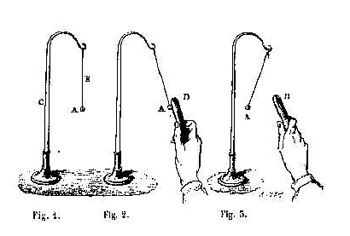
\includegraphics[scale=0.9]{./theorieDesChamps/MascartTraiteDElectriciteStatique1876}
\end{center}

L'expérience du pendule électrostatique peut se modéliser par des {\it forces électrostatiques} s'exerçant entre les particules chargées. Ce modèle suppose une {\it action à distance}.

% Dans un second temps, elle peut se modéliser par  en disant qu'une particule chargée crée un champ électrostatique en tout point de l'espace et qu'une particule chargée placé dans un champ électrostatique subit une force.

%\begin{minipage}[c]{.45\linewidth}
\begin{center}
Vision "Force de Coulomb"
\end{center}
Une charge électrique $Q_1$ exerce une force de Coulomb $\overrightarrow{F}_{Q_1/Q_2}$ sur la charge électrique $Q_2$

\begin{center}
\setlength{\unitlength}{1cm}
\begin{picture}(10,3)
\put(0.5,1.0){\circle{0.3}}
\put(0.3,0.3){$Q_1$}
%\put(0.5,1.0){\vector(1,0){1.36}}
%\put(1.2,1.3){$\overrightarrow{F}_{Q_2/Q_1}$}
\put(5.5,1.0){\circle{0.5}}
\put(5.3,0.2){$Q_2$}
\put(5.5,1.0){\vector(-1,0){1.36}}
\put(3.7,1.3){$\overrightarrow{F}_{Q_1/Q_2}$}
\end{picture}
\end{center}
%On peut alors se demander comment l'information de la présence de $Q_1$ parvient à $Q_2$, y a-t-il quelque chose qui se propage entre les charges ? Cette question peut être simplifiée en disant que les charges créent un champ dans tout l'espace et qu'elle sont sensibles à ce champ.
%\end{minipage}\hfill\begin{minipage}[c]{.45\linewidth}

%%%%%%%%%%%%%%%%%%%%%%%%%%%%%%%%%%%%%%%%%%%%%%%%%%%%%%%%%%%%%%%%%%%%%%%%%%%%

%
%
%%%%%%%%%%%%%%%%%%%%%
\section{Champ électrostatique}
%%%%%%%%%%%%%%%%%%%%%
%
%\subsection{Définition}
L'expérience du pendule électrostatique peut se modéliser par des {\it forces électrostatiques} s'exerçant entre les particules chargées. Ce modèle suppose une {\it action à distance}. La notion de champs permet de modéliser cette action entre les charges électriques : une charge électrique crée un champ dans tout l'espace. Le champ exercent une force sur les charges électriques.

\begin{center}
Vision "Champ électrique"
\end{center}
Une charge électrique $Q_1$ crée un champ électrique $\overrightarrow{E}$ dans tout l'espace.

\begin{center}
\setlength{\unitlength}{1cm}
\begin{picture}(10,3)
\put(0.5,1.0){\circle{0.3}}
\put(0.3,0.3){$Q_1$}
\put(5.5,1.0){\vector(-1,0){1.36}}
\put(3.7,1.3){$\overrightarrow{E}$}
\end{picture}
\end{center}

Le champ électrique $\overrightarrow{E}$ exerce une force $\overrightarrow{F}_{\overrightarrow{E}/Q_2}$ sur la charge électrique $Q_2$

\setlength{\unitlength}{1cm}
\begin{picture}(10,3)
\put(5.5,1.0){\circle{0.5}}
\put(5.3,0.2){$Q_2$}
\put(5.5,1.0){\vector(-1,0){1.36}}
\put(3.7,1.3){$\overrightarrow{F}_{\overrightarrow{E}/Q_2}$}
\end{picture}

Le champ créé par une charge électrique est à priori un outil purement mathématique, un artifice de calcul bien pratique. L'existence de ce "champ électrique" est à priori hypothétique. Néanmoins, son existence permet d'interpréter la transmission de "l'information de présence" entre les charges, de lever l'hypothèse d'une transmission d'information instantanée et immatérielle entre les charges.

%%%%%%%%%%%%%%%%%%%%%%%%%%%%%%%%%%%%%%%%%%%%%%%%%%%%%%%%%%%%%%%%%%%%%%%%%%%%

%
%
%%%%%%%%%%%%%%%%%%%%%
\section{Champ magnétique}
%%%%%%%%%%%%%%%%%%%%%
%
Les aimants exercent entre eux des forces magnétiques.

\begin{center}
%
%%%%%%%%%%%%%%%%%%%%%        PERSONNAGE AU BORD D'UNE MARE
%  DÉFINITIONS

\tikzset{
  feuillage/.style = {decoration={random steps, segment length=0.4mm}, decorate},
  tronc/.style   = {decoration={random steps, segment length=2mm, amplitude=0.2mm}, decorate}}

\tikzset{  arbre/.pic={ \foreach \w/\f in {0.3/30,0.2/50,0.1/70} { \fill [brown!\f!black, tronc] (-\w/2,0) rectangle +(\w,3); } \foreach \n/\f in {1.4/40,1.2/50,1/60,0.8/70,0.6/80,0.4/90} { \fill [green!\f!black, feuillage](0,3) ellipse (\n/1.5 and \n); }}}

\tikzset{  personnage/.pic={ { \fill [black] (0,0)ellipse(0.25 and 0.55); } 
  { \fill [black](0,0.75)circle(0.2); }
    % jambe et pieds
  {\fill [rounded corners=2pt] (0.1,-0.3)rectangle(-0.1,-1.5);}
  {\fill [rounded corners=2pt] (0.3,-1.4)rectangle(-0.1,-1.5);}
    % bras
  {\fill [rounded corners=2pt, rotate=-15] (-0.1,0.42)rectangle(0.5,0.29);}
  {\fill [rounded corners=2pt] (0.44,0.17)rectangle(1,0.29);}}}

\begin{tikzpicture}%[scale=0.5]
    %  Ciel
  \shade[bottom color=cyan!60!black, top color=blue!20!white] (0,0) rectangle (7.5,2.2);
    %  Sol
  \shade[bottom color=green!50!black, top color=green!70!black] (0,0.5) rectangle (7.5,-1);
    %  Mare
 % \shade[bottom color=blue!50!white, top color=cyan!60!black] (3.7,-0.15) ellipse (2.5 and 0.3);
    %  Arbre
 % \pic at (2,2)    {arbre};

    %  Personnage
  \begin{scope}[xshift=1 cm,yshift=0.6 cm]
    % corps et tête
 \fill [black] (0,0)ellipse(0.12 and 0.27);
 \fill [black](0,0.37)circle(0.1);
    % jambe et pieds
 \fill [rounded corners=2pt] (0.05,-0.15)rectangle(-0.05,-0.75);
 \fill [rounded corners=2pt] (0.15,-0.7)rectangle(-0.05,-0.75);
    % bras
 \fill [rounded corners=2pt, rotate=-15] (-0.1,0.22)rectangle(0.28,0.15);
 \fill [rounded corners=2pt] (0.22,0.08)rectangle(0.5,0.14);
   % Balle
 \fill[red] (0.5,0.05) circle(0.05);
  \end{scope}

\end{tikzpicture}

%%%%%%%%%%%%%%%%%%%%%%%%%%%%%%%%%%%%%%%%%%%%%%%%%%%%%%%%%%%%%%%%%%%%%%%%%%%%%%%%

\texttt{FIGURE : aimants, bousole}
\end{center}

De la même façon que pour l'électrostatique, les physiciens vont introduire le champ magnétique afin de "nommer à priori" le "médiateur" entre les aimants "expliquant" leurs interactions.

\begin{center}
%
%%%%%%%%%%%%%%%%%%%%%        PERSONNAGE AU BORD D'UNE MARE
%  DÉFINITIONS

\tikzset{
  feuillage/.style = {decoration={random steps, segment length=0.4mm}, decorate},
  tronc/.style   = {decoration={random steps, segment length=2mm, amplitude=0.2mm}, decorate}}

\tikzset{  arbre/.pic={ \foreach \w/\f in {0.3/30,0.2/50,0.1/70} { \fill [brown!\f!black, tronc] (-\w/2,0) rectangle +(\w,3); } \foreach \n/\f in {1.4/40,1.2/50,1/60,0.8/70,0.6/80,0.4/90} { \fill [green!\f!black, feuillage](0,3) ellipse (\n/1.5 and \n); }}}

\tikzset{  personnage/.pic={ { \fill [black] (0,0)ellipse(0.25 and 0.55); } 
  { \fill [black](0,0.75)circle(0.2); }
    % jambe et pieds
  {\fill [rounded corners=2pt] (0.1,-0.3)rectangle(-0.1,-1.5);}
  {\fill [rounded corners=2pt] (0.3,-1.4)rectangle(-0.1,-1.5);}
    % bras
  {\fill [rounded corners=2pt, rotate=-15] (-0.1,0.42)rectangle(0.5,0.29);}
  {\fill [rounded corners=2pt] (0.44,0.17)rectangle(1,0.29);}}}

\begin{tikzpicture}%[scale=0.5]
    %  Ciel
  \shade[bottom color=cyan!60!black, top color=blue!20!white] (0,0) rectangle (7.5,2.2);
    %  Sol
  \shade[bottom color=green!50!black, top color=green!70!black] (0,0.5) rectangle (7.5,-1);
    %  Mare
 % \shade[bottom color=blue!50!white, top color=cyan!60!black] (3.7,-0.15) ellipse (2.5 and 0.3);
    %  Arbre
 % \pic at (2,2)    {arbre};

    %  Personnage
  \begin{scope}[xshift=1 cm,yshift=0.6 cm]
    % corps et tête
 \fill [black] (0,0)ellipse(0.12 and 0.27);
 \fill [black](0,0.37)circle(0.1);
    % jambe et pieds
 \fill [rounded corners=2pt] (0.05,-0.15)rectangle(-0.05,-0.75);
 \fill [rounded corners=2pt] (0.15,-0.7)rectangle(-0.05,-0.75);
    % bras
 \fill [rounded corners=2pt, rotate=-15] (-0.1,0.22)rectangle(0.28,0.15);
 \fill [rounded corners=2pt] (0.22,0.08)rectangle(0.5,0.14);
   % Balle
 \fill[red] (0.5,0.05) circle(0.05);
  \end{scope}

\end{tikzpicture}

%%%%%%%%%%%%%%%%%%%%%%%%%%%%%%%%%%%%%%%%%%%%%%%%%%%%%%%%%%%%%%%%%%%%%%%%%%%%%%%%

\texttt{FIGURE : ligne de champ}
\end{center}
%%%%%%%%%%%%%%%%%%%%%%%%%%%%%%%%%%%%%%%%%%%%%%%%%%%%%%%%%%%%%%%%%%%%%%%%%%%%

%
%
%%%%%%%%%%%%%%%%%%%%%
\section{Champ gravitationnel}
%%%%%%%%%%%%%%%%%%%%%
%
%\subsection{Définition}

De la même façon que l'on définit le champ électrostatique, on définit le champ gravitationnel.

%Un champ est la donnée de sa valeur en tout point de l'espace. Cette valeur peut être scalaire ou vectoriel. Elle peut éventuellement être variable au cours du temps, elle est généralement variable dans l'espace.

%%%%%%%%%%%%%%%%%%%%%%%%%%%%%%%%%%%%%%%%%%%%%%%%%%%%%%%%%%%%%%%%%%%%%%%%%%%%

%

%%%%%%%%%%%%%%%%%%%%%
%\section{Propriétés des ondes électromagnétique}
\section{Ondes électromagnétiques}
%%%%%%%%%%%%%%%%%%%%%

\subsection{Champ électrique et champ magnétique}

Au début du XIX$^\text{ème}$ siècle, les expériences de Hans Christian Oersted montrent un lien intime entre les forces magnétiques et les forces électriques : les 

Les équations de maxwell vont établir un lien entre les champs magnétique et électrique : non seuleument ces champs sont créés par les charges électrique, les aimants et les charges en mouvement, mais un champ électrique est créé par un champ magnétique variable au cours du temps et un champ magnétique est créé par un champ électrique variable au cours du temps.

%\begin{center}
\[
\overrightarrow{E} \text{ variable au cours du temps } \Rightarrow \text{ création de } \overrightarrow{B}
\]
\[
\overrightarrow{B} \text{ variable au cours du temps } \Rightarrow \text{ création de } \overrightarrow{E}
\]
%\end{center}

%\vspace{0.2cm}

\subsection{Ondes électromagnétiques et lumière}

De ces dernières propriétés découlent l'existence d'ondes électromagnétiques dont la vitesse peut être calculée en fonction des constantes électriques et magnétiques apparaissant dans les équations de Maxwell. La valeur calculée, correspondant à la valeur de la vitesse de la lumière alors connue à l'époque.

Ces ondes se propage dans le vide et dans les milieux transparent.Leur identification avec la lumière achèvera l'unification des phénomènes électriques, magnétiques et lumineux.

%%%%%%%%%%%%%%%%%%%%%%%%%%%%%%%%%%%%%%%%%%%%%%%%%%%%%%%%%%%%%%%%%%%%%%%%%%%%%

%
%

%
\chapter{Physique quantique}
%

%%%%%%%%%%%%%%%%%%%%%
\section{Étymologie}
%%%%%%%%%%%%%%%%%%%%%
%
%\subsection{Ondes et particules}
\subsection{Particules élémentaire}
%\subsection{Lumière et matière}

\subsubsection{Matière et rayonnement}

\begin{itemize}[leftmargin=1cm, label=\ding{32}, itemsep=1pt]
\item électron
\item photon
\item proton
\item neutron
\end{itemize}

\subsubsection{Modèle standard}

\begin{itemize}[leftmargin=1cm, label=\ding{32}, itemsep=1pt]
\item quark
\item gluon
\item higgs
\item neutrino
\end{itemize}



\subsection{Quanton}
%

\begin{itemize}[leftmargin=1cm, label=\ding{32}, itemsep=1pt]
\item quantique
\item quanton
\end{itemize}




%%%%%%%%%%%%%%%%%%%%%%%%%%%%%%%%%%%%%%%%%%%%%%%%%%%%%%%%%%%%%%%%%%%%%%%%%%%%%%%%

%

%%%%%%%%%%%%%%%%%%%%%%%%%%%%%%%%%%%%%%%%%%%%

\section{Définitions}
  \subsection{Observateur et référentiel}

Pour étudier un mouvement, un {\it observateur} doit mesurer la position de l'objet en mouvement au cours du temps. Il doit donc disposer d'une horloge (pour mesurer le temps) et d'un système de coordonnées spatiales (pour mesurer la position).

L'horloge et le système de coordonnées "attachés" à l'observateur est appelé {\it référentiel}


    \subsubsection{Exemple}
Un observateur détermine la vitesse du train en chronomètrant la durée mis par le train pour parcourir la distance séparant les deux arbres.

\begin{center}
%%%%%%%%%%%%%%%%%%%%%%%%%%%%%%%%%%%%%%%%%%%%%%%%%%%%%%%
%%%%%%%%%%%%%%%%%%%%%%%%%%%%%%%%%%%%%%%%%%%%%%%%%%%%%%%%%%%%%%%%%%%%
\def\scl{0.2}%scaling factor of the picture

\begin{tikzpicture}[
  scale=\scl,
  beige/.style={color=gray!20!brown!40!yellow!20!},
  orange/.style={color=red!70!yellow!70!},
  wagon/.style={green!70!brown!20!black!75!,draw=black,thick},
  porte/.style={red!70!yellow!70!,draw=gray!20!, ultra thin},
  porteMotrice/.style={rounded corners = .1pt,draw=gray!60!, ultra thin},
  essieux/.style={gray!20!brown!30!black!60!,draw=black!70!, ultra thin},
  vitre/.style={bottom color=gray!5!, top color=gray!90!, shading angle={90}, draw=white, ultra thin},
  grisEssieux/.style={gray!20!brown!30!black!60!}
]


  \shade[bottom color=blue!20!white, top color=cyan!60!black] (20,10)
    rectangle (-60,0);
  \shade[bottom color=green!60!black, top color=green!60!] (20,-5)
    rectangle (-60,.3);



  \begin{scope}[xshift=0 cm,yshift=0 cm]%, scale = 0.3
%
%         LIAISONS
%
 \draw[black!70!, very thin] % liaison souple 42, rigide 65 +-11
    (6.1,0.65) to[out=330,in=0] (6.3,0.53);

 \draw[black!70!, very thin] 
    (-6.1,0.65) to[out=210,in=0] (-6.55,0.53);

 \draw[black!70!, thin] 
    (-6.1,0.76) -- (-6.56,0.76);


 % BUTOIRS
 %(\t * 6.1, 0.75) rectangle (\t * 6.4, 0.9);
 %(\t * 6.4, 0.7) rectangle (\t * 6.45, 0.95);

 % ESSIEUX derrière les roues

  \foreach \x in {3.64, -3.64}
   {
 \fill[gray] 
  (\x - 0.65, 0.95) -- (\x + 0.65, 0.95) --
 (\x + 1.6, 0.27) -- (\x + 1.06, 0.15) -- (\x + 0.65, 0.25)
 -- (\x - 0.65, 0.25) -- (\x - 1.06, 0.15) -- (\x - 1.6, 0.27) -- cycle;
  }

%  ROUES

\def\hauteur{0.55}% de l'axe des roues
\foreach \x in {2.58, 4.7, -4.7, -2.58}
  {
 % gris essieux : gray!20!brown!30!black!50!
    \fill[gray!20!brown!20!black!60!] (\x, \hauteur) circle (0.45 cm);
    \fill[gray!20!brown!40!black!40!] (\x, \hauteur) circle (0.41 cm);
    \fill[gray!10!brown!30!black!60!] (\x, \hauteur) circle (0.38 cm);

% RESSORT

  \foreach \t in {-1,1}
  {
     \draw[decorate, decoration={snake, segment length=1.5pt, amplitude=1.2mm}, black!70!, thin]
       (\x + \t * 0.28, 0.75) -- (\x + \t * 0.28, 0.35);
    % RESSORT fixation supérieur
     \fill[gray!20!brown!20!black!70!]
       (\x + \t * 0.28 - .13, 0.9) rectangle (\x + \t * 0.28 + .13, 0.7);
  }
  }


 % ESSIEUX devant les roues

\def\y{0.2}
  \foreach \x in {3.64, -3.64}
{
  \foreach \t in {-1,1}
  {
  % détail
 \fill[essieux] (\x + \t*1.57, 0.95) -- (\x + \t*1.67, 0.45) --
 (\x + \t*1.57, 0.45) -- (\x + \t*1.4, 0.95) -- cycle;

  %  montants supérieur
 \fill[essieux] (\x + \t*1.5, 0.95) -- (\x + \t*1.5, 0.85) -- (\x + \t*1, 0.83) -- (\x + \t*0.67, 0.65)
 -- (\x + \t*0.6, 0.35) -- (\x + \t*0.45, 0.35) -- (\x + \t*0.6, 0.95) -- cycle;


    %  montant inférieur
 \fill[essieux] (\x + \t * 1.5,0.45) -- (\x + \t * 1.5,0.4) -- (\x + \t * 1.2,0.35) -- (\x + \t * 1,0.35)
 -- (\x + \t * 0.80,0.37) -- (\x + \t * 0.65,0.25) -- (\x + \t * 0.65,0.45) -- cycle;

 \fill[essieux] (\x + \t*1.06, \hauteur + 0.05) circle (0.17 cm);
 \fill[grisEssieux]
 (\x + \t*1.06 + 0.16, 0.45) rectangle (\x + \t*1.06 + -0.16, 0.37);
 \fill[essieux]
 (\x + \t*1.06 + 0.1, \hauteur + 0.05 + -0.1) rectangle (\x + \t*1.06 + -0.1, \hauteur + 0.05 + 0.1);
    \fill[essieux] (\x + \t*1.06, \hauteur + 0.05) circle (0.09 cm);
    \fill[essieux] (\x + \t*1.06, \hauteur + 0.05) circle (0.04 cm);

  }

    %  milieux
   \fill[essieux, rounded corners = 3pt]
  (\x-0.22, 0.9) -- (\x + 0.22, 0.9) -- (\x + 0.4, 0.4) -- (\x - 0.4, 0.4) -- cycle;

    %  milieux inférieur 
  \fill[grisEssieux]
  (\x - 0.62,0.5) -- (\x + 0.62,0.5) -- (\x + 0.62,0.25) -- (\x - 0.62,0.25) -- cycle;

  \foreach \t in {-1,1}    % silent bloc
  {
  \fill[brown!30!black!80!]
 (\x + \t * 0.42 - 0.1, 0.6) rectangle (\x + \t * 0.42 + 0.1, 0.4);
  \fill[essieux]
 (\x + \t * 0.42 - 0.1, 0.45) rectangle (\x + \t * 0.42 + 0.1, 0.3);
  }
}

 % DESSOUS

 \fill[black!60!] 
  (1.9, 0.95) -- (- 1.9, 0.95) -- (- 1.4, 0.40) -- (1.4, 0.40) -- cycle;

  \shade[bottom color=gray!10!brown!50!black!60!, top color=gray!20!brown!40!black!40!] % ombre centre cylindre
  (1.05, 0.45) rectangle (-1.05, 0.66);
  \shade[bottom color=gray!20!brown!40!black!40!, top color=gray!10!brown!30!black!60!]
  (1.05, 0.64) rectangle (-1.05, 0.85);

 \fill[black!60!] 
  (2, 0.9) -- (- 2, 0.9) -- (- 1.9, 0.75) -- (1.9, 0.75) -- cycle;
 \fill[black!60!] 
  (1.15, 0.55) -- (- 1.15, 0.55) -- (- 1.15, 0.3) -- (1.15, 0.3) -- cycle;


  \shade[bottom color=brown!40!black!80!, top color=gray!20!brown!40!black!40!, rounded corners = 3pt]% cylindre
  (1.05, 0.45) rectangle (-1.05, 0.66);
  \shade[bottom color=gray!20!brown!40!black!40!, top color=gray!10!brown!30!black!60!, rounded corners = 3pt]%, shading angle={90}
  (1.05, 0.64) rectangle (-1.05, 0.85);

  \foreach \t in {-1,1}
{
  \fill[essieux] % details 1
 (\t * 2, 0.9) -- (\t * 1.7, 0.9) -- (\t * 1.72, 0.5)
 -- (\t * 1.85, 0.5) --  cycle;
  \fill[essieux] % details 2
 (\t * 1.67, 0.9) -- (\t * 1.2, 0.9) -- (\t * 1.2, 0.45)
 -- (\t * 1.67, 0.45) --  cycle;
}

 % BUTOIRS
\foreach \t in {-1,1}
{
  \fill[color=gray!80!black] % 
 (\t * 6.1, 0.75) rectangle (\t * 6.4, 0.9);
  \fill[color=black!80!gray] % plaques
 (\t * 6.4, 0.7) rectangle (\t * 6.45, 0.95);
}

% BAS DE CAISSE

\foreach \t in {-1,1}
{

  \fill[essieux] % details
 (\t * 5.9, 0.9) -- (\t * 5.3, 0.9) -- (\t * 5.5, 0.3)
 -- (\t * 5.85, 0.3) --  cycle;

  \fill[essieux] % pare bufle
 (\t * 6.2, 0.43) -- (\t * 6.35, 0.33) -- (\t * 6.2, 0.3) --  cycle;
  \fill[grisEssieux] % pare bufle
 (\t * 5, 0.95) -- (\t * 6.2, 0.95) -- (\t * 6.2, 0.3) --  cycle;

  \fill[color=gray] % carrosserie
 (\t * 5, 0.95) -- (\t * 6.2, 0.95) -- (\t * 6.2, 0.6) --  cycle;
}


%
%     CORPS DE LA MOTRICE
%
% liaisons électriques entre caténaires
     \draw[black!70!, thin] (-2.4, 3.15) -- (3.9, 3.15);

     \draw[black!70!, thin] (-4.5, 3.05) -- (4.1, 3.05);


%isolant 1
  \foreach \x in {-4.1, -3.6, 3.6, 4.1}
     \draw[decorate, decoration={snake, segment length=.2pt, amplitude=0.2mm}, red!50!black, thin]
       (\x, 2.9) -- (\x, 3.15);
  \foreach \x in {-4.1, -3.6, 3.6, 4.1}
     \fill[gray]
       (\x - 0.1, 2.9) rectangle (\x + 0.1, 2.95);

%caténaire
\def\h{0.05}
  \foreach \x in {-4.1, 3.6}
  {
     \draw[gray, line width=.7pt] (\x + 0.6, 3.1+\h) -- (\x - 0.1, 3.1+\h);
     \draw[black!60!, line width=1pt] (\x + 0.5, 3.15+\h) -- (\x, 3.15+\h);

     \draw[gray, line width=.7pt] (\x + 0.55, 3.05+\h) -- (\x + 1.8, 3.1+\h);
     \draw[gray, line width=.1pt] (\x + 0.55, 3.13+\h) -- (\x  + 1.8, 3.13+\h);

     \draw[gray, line width=.3pt] (\x, 3.2+\h) -- (\x  + 1.8, 3.15+\h);
     \draw[gray, line width=.1pt] (\x, 3.2+\h) -- (\x  + .8, 3.25+\h) -- (\x  + 1.7, 3.2+\h);
     \draw[gray, line width=.3pt] (\x  + .8, 3.18+\h) -- (\x  + .8, 3.28+\h);

  \fill[gray, draw=black!70!, thin, rounded corners = 1pt]% coude
 (\x + 1.8, 3.05+\h) -- (\x + 1.83, 3.1+\h) -- (\x + 1.78, 3.2+\h) -- (\x + 1.65, 3.2+\h)
 -- (\x + 1.68, 3.15+\h) -- cycle;

  }
  \foreach \x in {-4, 3.7}
  {
  \fill[gray, line width=2pt]% support et capteurs
 (\x-0.1, 3.28+\h) -- (\x+0.1, 3.28+\h) -- (\x, 3.17+\h)  -- cycle;
     \draw[gray, line width=.7pt] (\x-0.07, 3.28+\h) -- (\x-0.13, 3.28+\h);
     \draw[gray, line width=.7pt] (\x+0.07, 3.28+\h) -- (\x+0.13, 3.28+\h);
  }

% ÉLÉMENTS CATÉNAIRES

%isolant 2 à gauche
  \foreach \x in {-2.1, -2.35}
     \draw[decorate, decoration={snake, segment length=.2pt, amplitude=.4mm}, red!50!black, thin]
       (\x, 2.9) -- (\x, 3.15);
     \fill[gray] (-2.23 - 0.3, 2.9) rectangle (-2.23 + 0.3, 2.95);
     \fill[gray] (-2.23 - 0.3, 2.9) rectangle (-2.23 + 0.3, 2.95);
%isolant 2 à droite
     \draw[decorate, decoration={snake, segment length=.2pt, amplitude=.4mm}, red!50!black, thin]
       (2.6, 2.9) -- (2.6, 3.08);
   %  \fill[gray] (2.6 - 0.3, 2.9) rectangle (2.6 + 0.3, 2.95);
% boitier
  \foreach \x in {-4.6, 2.8}
{
     \draw[decorate, decoration={snake, segment length=.2pt, amplitude=0.1mm}, red!50!black, thin]
       (\x+0.25, 3.05) -- (\x+0.6, 3.05);

     \fill[gray] (\x - 0.28, 3.12) -- (\x + 0.28, 3.12)
     -- (\x + 0.3, 3.07)
     -- (\x + 0.28, 2.95) -- (\x - 0.28, 2.95) -- (\x - 0.3, 3.07) -- cycle;

     \draw[gray, ultra thick] (\x + 0.18, 3.12) -- (\x + 0.18, 2.5);
     \draw[gray, ultra thick] (\x, 3.12) -- (\x, 2.5);
}


% trompes
\foreach \t in {-1, 1}
  {
  \fill[gray]%
 (\t * 5.35,2.92) -- (\t * 5.75, 3) -- (\t * 5.75, 2.85)  -- cycle;
  \draw[gray, thin] (\t * 5.45, 3) -- (\t * 5.45, 2.85);
  }


% TOIT

  \fill[color=black!50!] % toit 1
 (1.9, 2.9) -- (-1.9, 2.9) -- (-1.65, 3.3) -- (1.65, 3.3) -- cycle;
\def\demi{0.25}
\foreach \x in{ -1.2, -0.6, 0, 0.6, 1.2 }
  \fill[black!30!] % grilles
 (\x - \demi, 3.1) rectangle (\x + \demi, 2.9);

  \fill[color=gray] % toit 2
 (4.5, 2.9) -- (5.75, 2.85) -- (5.85, 2.7) -- (-5.85, 2.7) -- 
 (-5.75, 2.85) -- (-4.5, 2.9) -- cycle;

  \fill[beige,draw=gray!50!, ultra thin] % carosserie
 (5.85, 2.7) -- (5.9, 2.55) -- (5.8, 2.1) -- (6.25, 1.95) -- (6.32, 1.75)
 -- (6.2, 0.9) --  (-6.2, 0.9) -- (-6.32, 1.75) -- (-6.25, 1.95)
 -- (-5.8, 2.1) -- (-5.9, 2.55) -- (-5.85, 2.7) -- cycle;

  \fill[orange] % décoration
 (4.45, 2.55) -- (3.85, 1.8) -- (6.32, 1.75) -- (6.35, 1.6) -- (3.35, 1.6) -- (4.1, 2.4) 
 -- (-4.1, 2.4) -- (-3.35, 1.6) -- (-6.27, 1.6) -- (-6.32, 1.75) -- (-3.85, 1.8) -- (-4.45, 2.55) -- cycle;


  \fill[color=gray!50!] % grille
 (3.2,1.6) -- (3.2, 2.4) -- (-3.2,2.4) -- (-3.2, 1.6) --  cycle;

  %  FEUX

\foreach \t in {-1,1}
{
  \fill[color=gray!50!,draw=gray, ultra thin]
 (\t * 6.3,1.67) rectangle (\t * 6.37, 1.53);
  \fill[color=brown!20!red!50!yellow!70!,draw=gray, ultra thin]
 (\t * 6.2,1.7) -- (\t * 6.3, 1.7) -- (\t * 6.3, 1.4) -- (\t * 6.1, 1.4) -- cycle;
  \fill[color=gray]
 (\t * 6.23,1.4) rectangle (\t * 6.28, 1.2);
}


\foreach \t in {-1,1}
{
      % PARE BRISE ET GRIS AUTOUR

  \fill[color=gray] % gris
 (\t*4.5, 2.55) -- (\t*5.9, 2.55) -- (\t*5.8, 2.1) -- (\t*4.15, 2.1) --  cycle;
  \shade[bottom color=gray!5!, top color=gray!90!, shading angle={90}, draw=black] % vitre
 (\t*5.8, 2.54) -- (\t*5.87, 2.54) -- (\t*5.8, 2.12) -- (\t*5.6, 2.12) --  cycle;

  \fill[color=gray] % gris
 (\t*4.5, 2.55) -- (\t*5.85, 2.55) -- (\t*5.65, 2.1) -- (\t*4.15, 2.1) --  cycle;

      % PORTES

    \draw[porteMotrice]
 (\t*4.55, 1.3) rectangle (\t*5, 2.6);

    \draw[draw=gray!40!,very thin] % marches
 (\t*4.62, 1.03) rectangle (\t*4.93, 1.15);

    \draw[color=gray] (\t*4.5, 1.03) -- (\t*4.5, 2.3); % rampes
    \draw[color=gray] (\t*5.05, 1.03) -- (\t*5.05, 2.3);

  \shade[bottom color=white, top color=black!80!, shading angle={90}]
   (\t*4.65, 2.12) rectangle (\t*4.9, 2.52); % vitres
}

  % RAIL

  % RAIL
  \fill[color=brown!20!gray!40!black]
 %(-8.75, 0.02) rectangle (8.75, -0.05); WAGON
 (20, 0.13) rectangle (-6.7, 0.06);

  \end{scope}
%
%
%%%%%%%%%%%%%%%%%%%%%%%%%%%%%%%%%%%%%%%%%%%%%%%%%%%%%%%%%%%%%%%%%%%%%

         %    WAGONS

%%%%%%%%%%%%%%%%%%%%%%%%%%%%%%%%%%%%%%%%%%%%%%%%%%%%%%%%%%%%%%%%%%%%

  \begin{scope}[xshift=-15.5 cm,yshift=0.11 cm]%, scale = 0.3
%
%         LIAISONS
% 
  \fill[color=gray,draw=gray!20!, ultra thin] % fixation souflets
 (8.65, 0.9) rectangle (-8.65, 2.2);

 \draw[black!70!, very thin] % liaison souple
    (8.3,0.65) to[out=330,in=180] (9,0.42);
 \draw[black!70!, very thin] 
    (-8.3,0.65) to[out=210,in=0] (-9,0.42);

  \foreach \t in {-1, 1}
  {
  \fill[color=black!80!,draw=gray!80!, ultra thin] % 
 (8.65 * \t, 0.9) rectangle (8.75 * \t, 2.3); % gris foncé, souflets

    \coordinate (A) at (8.3 * \t,0.65) ;
    \coordinate (B) at (9 * \t,0.65) ;
 \draw[black!70!, thin] 
    (A) -- (B);

  }

 % BUTOIRS
  \foreach \t in {-1, 1}
  {
  \fill[color=gray,draw=gray!50!, ultra thin] % 
 (8.3 * \t, 0.65) rectangle (\t * 8.66, 0.8);
  \fill[color=gray!50!black] % 
 (\t * 8.66, 0.6) rectangle (\t * 8.7, 0.85);
  }
%
%     CORPS DU WAGON
%
  \shade[bottom color=black!70!, top color=gray!50!, rounded corners=1pt]  % toit
 (-8.6, 2) rectangle (8.6, 2.7);

  \fill[color=gray!20!] % gris clair
 (-8.6, 2.1) rectangle (8.6, 2.4);
  \fill[color=gray!20!] % gris clair
 (-8.6, 0.8) rectangle (8.6, 1.25);

  \fill[color=gray!5!] % blanc
 (-8.6, 2.1) rectangle (8.6, 2.2);
  \fill[color=gray!5!] % blanc
 (-8.6, 1.25) rectangle (8.6, 1.3);

%  ROUES

\def\hauteur{0.35}% de l'axe des roues
\foreach \x in {5.45, 7.1, -5.45, -7.1}
  {
 % gris essieux : gray!20!brown!30!black!50!
    \fill[gray!20!brown!20!black!60!] (\x, \hauteur) circle (0.35 cm);
    \fill[gray!20!brown!40!black!40!] (\x, \hauteur) circle (0.31 cm);
    \fill[gray!10!brown!30!black!60!] (\x, \hauteur) circle (0.28 cm);
  \fill[color=gray,draw=black!70!, ultra thin] %,rotate=45
 (\x + 0.1, \hauteur + -0.1) rectangle (\x -0.1, \hauteur + 0.1);

  \fill[color=gray,draw=gray!20!, ultra thin] (\x, \hauteur) circle (0.08 cm);
  }
 % ESSIEUX
\def\y{0.2}
  \foreach \x in {6.25, -6.25}
   {
 \fill[black!20!gray!70!,draw=gray!20!, ultra thin] 
  (\x - 0.35, 0.2) rectangle (\x + 0.35, 0.45);

 \fill[black!20!gray!70!,draw=gray!20!, ultra thin] 
  (\x - 0.45, 0.45) rectangle (\x + 0.45, 0.55);

 \fill[black!20!gray!70!,draw=gray!20!, ultra thin] 
  (\x - 0.35, 0.55) rectangle (\x + 0.35, 0.7);

    \coordinate (A) at (\x + -0.75,\y + 0.45) ;
      \coordinate (B) at (\x - 0.2,\y + 0.27) ;
      \coordinate (C) at (\x + 0.2,\y + 0.27) ;
    \coordinate (D) at (\x + 0.75,\y + 0.45) ;
    \coordinate (E) at (\x + 0.75,\y + 0.32) ;
      \coordinate (F) at (\x + 0.2,\y + 0) ;
      \coordinate (G) at (\x - 0.2,\y + 0) ;
    \coordinate (H) at (\x - 0.75,\y + 0.32) ;
 \fill[black!20!gray!70!,draw=gray!20!, ultra thin] 
    (A) to[out=0,in=180] (B) to[out=0,in=180] (C) to[out=0,in=180]
    (D) to[out=-90,in=90] (E) to[out=180,in=0] (F) to[out=180,in=0]
    (G) to[out=180,in=0] (H) -- cycle;
  }

% MARCHE
  \foreach \t in {-1, 1}
  {
    \draw[draw=black!70!,very thin] % montant
 (\t * 7.9, 0.35) -- (\t * 7.8, 0.6);
    \draw[draw=black!70!,very thin] % montant
 (\t * 7.4, 0.35) -- (\t * 7.5, 0.6);
    \draw[draw=black!70!,thin] % marche
 (\t * 7.3, 0.35) -- (\t * 8, 0.35);
  }

% BAS DE CAISSE

  \fill[color=gray, rounded corners=1pt] % gris Foncé
    (-8.6, .8) rectangle (8.6, .65);


  \foreach \t in {-1, 1}
  \fill[color=gray, rounded corners=1pt] % gris Foncé
    (\t * 8.6, .7) -- (\t * 8.4, .45) -- (\t * 6.8, .45) -- (\t * 6.8, .7) -- cycle;
  \fill[color=gray, rounded corners=1pt] % gris Foncé
    (5.6, .7) -- (5.5, .45) -- (-5.5, .45) -- (-5.6, .7) -- cycle;

      % FENÊTRES
  \foreach \t in {1.05, 2.55, 4.05, 5.55}
  {
  \shade[vitre]
   (\t, 1.36) rectangle (\t + 1, 2.03);
  \shade[vitre]
   (-\t, 1.36) rectangle (-\t - 1, 2.03);
  }
  \shade[vitre]
   (-0.5, 1.36) rectangle (0.5, 2.03);

      % PORTES
  \foreach \t in {-1, 1}
  {

    \fill[gray!80!black] % marche
 (\t * 7.45, 0.53) rectangle (\t * 7.9, 0.7);
    \fill[gray!60!black] % marche
 (\t * 7.45, 0.53) rectangle (\t * 7.9, 0.57);

  \fill[gray!80!black]
 (\t * 7.2, 0.7) rectangle (\t * 8, 2.15);
  \fill[porte]
 (\t * 7.25, 0.8) rectangle (\t * 7.6, 2.05);
  \fill[porte]
 (\t * 7.45, 0.8) rectangle (\t * 7.9, 2.05);

  \shade[bottom color=gray!5!, top color=gray!90!, shading angle={90}, draw=black, ultra thin] % fenêtre
   (\t * 7.6, 1.4) rectangle (\t * 7.8, 1.9);

    \draw[gray!10!]
 (\t * 7.75, 1.15) -- (\t * 7.85, 1.1); % poignée
  }

  % RAIL WAGON
  \fill[color=brown!20!gray!40!black]
 (-8.85, 0.02) rectangle (8.85, -0.05);

  \end{scope}
%
%
%
%%%%%%%%%%%%%%%%%%%%%%%%%%%%%%%%%%%%%%%%%%%%%%%%%%%%%%%%%%%%%%%%%%%%%

         %    WAGON  2

%%%%%%%%%%%%%%%%%%%%%%%%%%%%%%%%%%%%%%%%%%%%%%%%%%%%%%%%%%%%%%%%%%%%

  \begin{scope}[xshift=-33.2 cm,yshift=0.11 cm]%, scale = 0.3
%
%         LIAISONS
% 
  \fill[color=gray,draw=gray!20!, ultra thin] % fixation souflets
 (8.65, 0.9) rectangle (-8.65, 2.2);

 \draw[black!70!, very thin] % liaison souple
    (8.3,0.65) to[out=330,in=180] (9,0.42);
 \draw[black!70!, very thin] 
    (-8.3,0.65) to[out=210,in=0] (-9,0.42);

  \foreach \t in {-1, 1}
  {
  \fill[color=black!80!,draw=gray!80!, ultra thin] % 
 (8.65 * \t, 0.9) rectangle (8.75 * \t, 2.3); % gris foncé, souflets
    \coordinate (A) at (8.3 * \t,0.65) ;
    \coordinate (B) at (9 * \t,0.65) ;
 \draw[black!70!, thin] 
    (A) -- (B);
  }

  \fill[color=black!80!] % 
 (8.75, 0.95) rectangle (8.95, 2.25); % gris foncé, souflet liaison
 % BUTOIRS
  \foreach \t in {-1, 1}
  {
  \fill[color=gray,draw=gray!50!, ultra thin] % 
 (8.3 * \t, 0.65) rectangle (\t * 8.66, 0.8);
  \fill[color=gray!50!black] % 
 (\t * 8.66, 0.6) rectangle (\t * 8.7, 0.85);
  }
%
%     CORPS DU WAGON
%
  \shade[bottom color=black!70!, top color=gray!50!, rounded corners=1pt]  % toit
 (-8.6, 2) rectangle (8.6, 2.7);

  \fill[color=gray!20!] % gris clair
 (-8.6, 2.1) rectangle (8.6, 2.4);
  \fill[color=gray!20!] % gris clair
 (-8.6, 0.8) rectangle (8.6, 1.25);

  \fill[color=gray!5!] % blanc
 (-8.6, 2.1) rectangle (8.6, 2.2);
  \fill[color=gray!5!] % blanc
 (-8.6, 1.25) rectangle (8.6, 1.3);

%  ROUES

\def\hauteur{0.35}% de l'axe des roues
\foreach \x in {5.45, 7.1, -5.45, -7.1}
  {
 % gris essieux : gray!20!brown!30!black!50!
    \fill[gray!20!brown!20!black!60!] (\x, \hauteur) circle (0.35 cm);
    \fill[gray!20!brown!40!black!40!] (\x, \hauteur) circle (0.31 cm);
    \fill[gray!10!brown!30!black!60!] (\x, \hauteur) circle (0.28 cm);
  \fill[color=gray,draw=black!70!, ultra thin] %,rotate=45
 (\x + 0.1, \hauteur + -0.1) rectangle (\x -0.1, \hauteur + 0.1);

  \fill[color=gray,draw=gray!20!, ultra thin] (\x, \hauteur) circle (0.08 cm);
  }
 % ESSIEUX
\def\y{0.2}
  \foreach \x in {6.25, -6.25}
   {
 \fill[black!20!gray!70!,draw=gray!20!, ultra thin] 
  (\x - 0.35, 0.2) rectangle (\x + 0.35, 0.45);

 \fill[black!20!gray!70!,draw=gray!20!, ultra thin] 
  (\x - 0.45, 0.45) rectangle (\x + 0.45, 0.55);

 \fill[black!20!gray!70!,draw=gray!20!, ultra thin] 
  (\x - 0.35, 0.55) rectangle (\x + 0.35, 0.7);

    \coordinate (A) at (\x + -0.75,\y + 0.45) ;
      \coordinate (B) at (\x - 0.2,\y + 0.27) ;
      \coordinate (C) at (\x + 0.2,\y + 0.27) ;
    \coordinate (D) at (\x + 0.75,\y + 0.45) ;
    \coordinate (E) at (\x + 0.75,\y + 0.32) ;
      \coordinate (F) at (\x + 0.2,\y + 0) ;
      \coordinate (G) at (\x - 0.2,\y + 0) ;
    \coordinate (H) at (\x - 0.75,\y + 0.32) ;
 \fill[black!20!gray!70!,draw=gray!20!, ultra thin] 
    (A) to[out=0,in=180] (B) to[out=0,in=180] (C) to[out=0,in=180]
    (D) to[out=-90,in=90] (E) to[out=180,in=0] (F) to[out=180,in=0]
    (G) to[out=180,in=0] (H) -- cycle;
  }

% MARCHE
  \foreach \t in {-1, 1}
  {
    \draw[draw=black!70!,very thin] % montant
 (\t * 7.9, 0.35) -- (\t * 7.8, 0.6);
    \draw[draw=black!70!,very thin] % montant
 (\t * 7.4, 0.35) -- (\t * 7.5, 0.6);
    \draw[draw=black!70!,thin] % marche
 (\t * 7.3, 0.35) -- (\t * 8, 0.35);
  }

% BAS DE CAISSE

  \fill[color=gray, rounded corners=1pt] % gris Foncé
    (-8.6, .8) rectangle (8.6, .65);


  \foreach \t in {-1, 1}
  \fill[color=gray, rounded corners=1pt] % gris Foncé
    (\t * 8.6, .7) -- (\t * 8.4, .45) -- (\t * 6.8, .45) -- (\t * 6.8, .7) -- cycle;
  \fill[color=gray, rounded corners=1pt] % gris Foncé
    (5.6, .7) -- (5.5, .45) -- (-5.5, .45) -- (-5.6, .7) -- cycle;

      % FENÊTRES
  \foreach \t in {1.05, 2.55, 4.05, 5.55}
  {
  \shade[vitre]
   (\t, 1.36) rectangle (\t + 1, 2.03);
  \shade[vitre]
   (-\t, 1.36) rectangle (-\t - 1, 2.03);
  }
  \shade[vitre]
   (-0.5, 1.36) rectangle (0.5, 2.03);

      % PORTES
  \foreach \t in {-1, 1}
  {

    \fill[gray!80!black] % marche
 (\t * 7.45, 0.53) rectangle (\t * 7.9, 0.7);
    \fill[gray!60!black] % marche
 (\t * 7.45, 0.53) rectangle (\t * 7.9, 0.57);

  \fill[gray!80!black]
 (\t * 7.2, 0.7) rectangle (\t * 8, 2.15);
  \fill[porte]
 (\t * 7.25, 0.8) rectangle (\t * 7.6, 2.05);
  \fill[porte]
 (\t * 7.45, 0.8) rectangle (\t * 7.9, 2.05);

  \shade[bottom color=gray!5!, top color=gray!90!, shading angle={90}, draw=black, ultra thin] % fenêtre
   (\t * 7.6, 1.4) rectangle (\t * 7.8, 1.9);

    \draw[gray!10!]
 (\t * 7.75, 1.15) -- (\t * 7.85, 1.1); % poignée
  }

  % RAIL WAGON
  \fill[color=brown!20!gray!40!black]
 (-8.85, 0.02) rectangle (8.85, -0.05);

  \end{scope}
%
%
%%%%%%%%%%%%%%%%%%%%%%%%%%%%%%%%%%%%%%%%%%%%%%%%%%%%%%%%%%%%%%%%%%%%%

         %    WAGON  3

%%%%%%%%%%%%%%%%%%%%%%%%%%%%%%%%%%%%%%%%%%%%%%%%%%%%%%%%%%%%%%%%%%%%

  \begin{scope}[xshift=-50.9 cm,yshift=0.11 cm]%, scale = 0.3
%
%         LIAISONS
% 
  \fill[color=gray,draw=gray!20!, ultra thin] % fixation souflets
 (8.65, 0.9) rectangle (-8.65, 2.2);

 \draw[black!70!, very thin] % liaison souple
    (8.3,0.65) to[out=330,in=180] (9,0.42);

 \draw[black!70!, very thin] 
    (-8.3,0.65) -- (-8.6,0.45);

  \foreach \t in {-1, 1}
  {
  \fill[color=black!80!,draw=gray!80!, ultra thin] % 
 (8.65 * \t, 0.9) rectangle (8.75 * \t, 2.3); % gris foncé, souflets
  }
  \fill[color=black!80!] % 
 (8.75, 0.95) rectangle (8.95, 2.25); % gris foncé, souflet liaison

    \coordinate (A) at (8.3,0.65) ;
    \coordinate (B) at (9,0.65) ;
 \draw[black!70!, thin] 
    (A) -- (B);

 % BUTOIRS
  \foreach \t in {-1, 1}
  {
  \fill[color=gray,draw=gray!50!, ultra thin] % 
 (8.3 * \t, 0.65) rectangle (\t * 8.66, 0.8);
  \fill[color=gray!50!black] % 
 (\t * 8.66, 0.6) rectangle (\t * 8.7, 0.85);
  }
%
%     CORPS DU WAGON
%
  \shade[bottom color=black!70!, top color=gray!50!, rounded corners=1pt]  % toit
 (-8.6, 2) rectangle (8.6, 2.7);

  \fill[color=gray!20!] % gris clair
 (-8.6, 2.1) rectangle (8.6, 2.4);
  \fill[color=gray!20!] % gris clair
 (-8.6, 0.8) rectangle (8.6, 1.25);

  \fill[color=gray!5!] % blanc
 (-8.6, 2.1) rectangle (8.6, 2.2);
  \fill[color=gray!5!] % blanc
 (-8.6, 1.25) rectangle (8.6, 1.3);

%  ROUES

\def\hauteur{0.35}% de l'axe des roues
\foreach \x in {5.45, 7.1, -5.45, -7.1}
  {
 % gris essieux : gray!20!brown!30!black!50!
    \fill[gray!20!brown!20!black!60!] (\x, \hauteur) circle (0.35 cm);
    \fill[gray!20!brown!40!black!40!] (\x, \hauteur) circle (0.31 cm);
    \fill[gray!10!brown!30!black!60!] (\x, \hauteur) circle (0.28 cm);
  \fill[color=gray,draw=black!70!, ultra thin] %,rotate=45
 (\x + 0.1, \hauteur + -0.1) rectangle (\x -0.1, \hauteur + 0.1);

  \fill[color=gray,draw=gray!20!, ultra thin] (\x, \hauteur) circle (0.08 cm);
  }
 % ESSIEUX
\def\y{0.2}
  \foreach \x in {6.25, -6.25}
   {
 \fill[black!20!gray!70!,draw=gray!20!, ultra thin] 
  (\x - 0.35, 0.2) rectangle (\x + 0.35, 0.45);

 \fill[black!20!gray!70!,draw=gray!20!, ultra thin] 
  (\x - 0.45, 0.45) rectangle (\x + 0.45, 0.55);

 \fill[black!20!gray!70!,draw=gray!20!, ultra thin] 
  (\x - 0.35, 0.55) rectangle (\x + 0.35, 0.7);

    \coordinate (A) at (\x + -0.75,\y + 0.45) ;
      \coordinate (B) at (\x - 0.2,\y + 0.27) ;
      \coordinate (C) at (\x + 0.2,\y + 0.27) ;
    \coordinate (D) at (\x + 0.75,\y + 0.45) ;
    \coordinate (E) at (\x + 0.75,\y + 0.32) ;
      \coordinate (F) at (\x + 0.2,\y + 0) ;
      \coordinate (G) at (\x - 0.2,\y + 0) ;
    \coordinate (H) at (\x - 0.75,\y + 0.32) ;
 \fill[black!20!gray!70!,draw=gray!20!, ultra thin] 
    (A) to[out=0,in=180] (B) to[out=0,in=180] (C) to[out=0,in=180]
    (D) to[out=-90,in=90] (E) to[out=180,in=0] (F) to[out=180,in=0]
    (G) to[out=180,in=0] (H) -- cycle;
  }

% MARCHE
  \foreach \t in {-1, 1}
  {
    \draw[draw=black!70!,very thin] % montant
 (\t * 7.9, 0.35) -- (\t * 7.8, 0.6);
    \draw[draw=black!70!,very thin] % montant
 (\t * 7.4, 0.35) -- (\t * 7.5, 0.6);
    \draw[draw=black!70!,thin] % marche
 (\t * 7.3, 0.35) -- (\t * 8, 0.35);
  }

% BAS DE CAISSE

  \fill[color=gray, rounded corners=1pt] % gris Foncé
    (-8.6, .8) rectangle (8.6, .65);


  \foreach \t in {-1, 1}
  \fill[color=gray, rounded corners=1pt] % gris Foncé
    (\t * 8.6, .7) -- (\t * 8.4, .45) -- (\t * 6.8, .45) -- (\t * 6.8, .7) -- cycle;
  \fill[color=gray, rounded corners=1pt] % gris Foncé
    (5.6, .7) -- (5.5, .45) -- (-5.5, .45) -- (-5.6, .7) -- cycle;

      % FENÊTRES
  \foreach \t in {1.05, 2.55, 4.05, 5.55}
  {
  \shade[vitre]
   (\t, 1.36) rectangle (\t + 1, 2.03);
  \shade[vitre]
   (-\t, 1.36) rectangle (-\t - 1, 2.03);
  }
  \shade[vitre]
   (-0.5, 1.36) rectangle (0.5, 2.03);

      % PORTES
  \foreach \t in {-1, 1}
  {

    \fill[gray!80!black] % marche
 (\t * 7.45, 0.53) rectangle (\t * 7.9, 0.7);
    \fill[gray!60!black] % marche
 (\t * 7.45, 0.53) rectangle (\t * 7.9, 0.57);

  \fill[gray!80!black]
 (\t * 7.2, 0.7) rectangle (\t * 8, 2.15);
  \fill[porte]
 (\t * 7.25, 0.8) rectangle (\t * 7.6, 2.05);
  \fill[porte]
 (\t * 7.45, 0.8) rectangle (\t * 7.9, 2.05);

  \shade[bottom color=gray!5!, top color=gray!90!, shading angle={90}, draw=black, ultra thin] % fenêtre
   (\t * 7.6, 1.4) rectangle (\t * 7.8, 1.9);

    \draw[gray!10!]
 (\t * 7.75, 1.15) -- (\t * 7.85, 1.1); % poignée
  }

  % RAIL WAGON
  \fill[color=brown!20!gray!40!black]
 (-9.1, 0.02) rectangle (8.85, -0.05);

  \end{scope}
%
\tikzset{
  treetop/.style = {decoration={random steps, segment length=0.2mm}, decorate},
  trunk/.style   = {decoration={random steps, segment length=1mm,
                    amplitude=0.2mm}, decorate}}

%  arbre à droite
       \fill [brown!50!black, trunk] (15,-1) rectangle (15.8,2);
       \fill [brown!60!black, trunk] (15.2,-1) rectangle (15.6,2);
     
       \fill [green!60!black, treetop](15,3) ellipse (1.5 and 2.25);
       \fill [green!40!black, treetop](15,3) ellipse (1 and 1.5);
     

%  arbre à gauche
       \fill [brown!30!black, trunk] (-55,-1) rectangle (-55.8,3);
       \fill [brown!60!black, trunk] (-55.2,-1) rectangle (-55.6,3);
     
       \fill [green!60!black, treetop](-55,3) ellipse (1.5 and 2.25);
       \fill [green!40!black, treetop](-55,3) ellipse (1 and 1.5);
     

%
\end{tikzpicture}
%

%%%%%%%%%%%%%%%%%%%%%%%%%%%%%%%%%%%%%%%%%%%%%%%%%%%%%%
%%%%%%%%%%%%%%%%%%%%%%%%%%%%%%%%%%%%%%%%%%%%%%%%%%%%%%%%%%%%%%%%%%%%
\def\scl{1}%scaling factor of the picture


\begin{tikzpicture}[
  scale=\scl,
  %wagon/.style={yellow!30!brown!20!,rounded corners,draw=black,thick},
  wagon/.style={green!70!brown!20!black!75!,draw=black,thick},
 % toit/.style={black!70!brown!20!,draw=gray,thick},
  %roue/.style={brown!20!black!70!,draw=black,thick},
  fenetre/.style={white,rounded corners = 2pt,draw=black, thick},
  porte/.style={color=red!70!yellow!70!,draw=gray!50!, ultra thin}
  ]

  \begin{scope}[xshift=0 cm,yshift=0 cm]%, scale = 0.3
%
%         LIAISONS
% 
  \fill[color=gray,draw=gray!20!, ultra thin] % souflet gris
 (8.65, 0.9) rectangle (-8.65, 2.2);

 \draw[black!70!, very thick] 
    (8.3,0.65) to[out=330,in=180] (8.75,0.42);
 \draw[black!70!, very thick] 
    (-8.3,0.65) to[out=210,in=0] (-8.75,0.42);

  \foreach \t in {-1, 1}
  {
  \fill[color=black!80!,draw=gray!80!, ultra thin, rounded corners=2pt] % 
 (8.65 * \t, 0.9) rectangle (8.75 * \t, 2.3); % gris foncé, souflet

    \coordinate (A) at (8.3 * \t,0.65) ;
    \coordinate (B) at (8.75 * \t,0.65) ;
 \draw[black!70!, ultra thick] 
    (A) -- (B);

  }

 % BUTOIRS
  \foreach \t in {-1, 1}
  {
  \fill[color=gray,draw=gray!50!, ultra thin] % 
 (8.3 * \t, 0.65) rectangle (\t * 8.66, 0.8);
  \fill[color=gray!50!black] % 
 (\t * 8.66, 0.6) rectangle (\t * 8.7, 0.85);
  }
%
%     CORPS DU WAGON
%
  \shade[bottom color=gray, top color=gray!10!, rounded corners]  % toit
 (-8.6, 2) rectangle (8.6, 2.7);

  \fill[color=gray!20!] % gris clair
 (-8.6, 2.1) rectangle (8.6, 2.4);
  \fill[color=gray!20!] % gris clair
 (-8.6, 0.8) rectangle (8.6, 1.25);

  \fill[color=gray!5!] % blanc
 (-8.6, 2.1) rectangle (8.6, 2.2);
  \fill[color=gray!5!] % blanc
 (-8.6, 1.25) rectangle (8.6, 1.3);


% Arriere roues
  %\foreach \x in {6.25, -6.25} \fill[brown!40!black] (\x - 0.85, 0.8) rectangle (\x + 0.85, 0.45);

%  ROUES
\def\hauteur{0.35}% de l'axe des roues
\tikzset{
  roue/.pic={
    \fill[black!20!gray!70!] (0, \hauteur) circle (0.35 cm);
    \fill[gray!20!] (0, \hauteur) circle (0.31 cm);
    \fill[black!20!gray!70!] (0, \hauteur) circle (0.28 cm);

  \fill[color=gray,draw=gray!20!, ultra thin] %,rotate=45
 (0.1, \hauteur + -0.1) rectangle (-0.1, \hauteur + 0.1);

  \fill[color=gray,draw=gray!20!, ultra thin] (0, \hauteur) circle (0.08 cm);

  }
}

  \pic at (5.45,0)    {roue};
  \pic at (7.1,0)    {roue};
  \pic at (-5.45,0)    {roue};
  \pic at (-7.1,0)    {roue};
 % ESSIEUX
\def\y{0.2}
  \foreach \x in {6.25, -6.25}
   {
 \fill[black!20!gray!70!,draw=gray!20!, ultra thin] 
  (\x - 0.35, 0.2) rectangle (\x + 0.35, 0.45);

 \fill[black!20!gray!70!,draw=gray!20!, ultra thin] 
  (\x - 0.45, 0.45) rectangle (\x + 0.45, 0.55);

 \fill[black!20!gray!70!,draw=gray!20!, ultra thin] 
  (\x - 0.35, 0.55) rectangle (\x + 0.35, 0.7);

    \coordinate (A) at (\x + -0.75,\y + 0.45) ;
      \coordinate (B) at (\x - 0.2,\y + 0.27) ;
      \coordinate (C) at (\x + 0.2,\y + 0.27) ;
    \coordinate (D) at (\x + 0.75,\y + 0.45) ;
    \coordinate (E) at (\x + 0.75,\y + 0.32) ;
      \coordinate (F) at (\x + 0.2,\y + 0) ;
      \coordinate (G) at (\x - 0.2,\y + 0) ;
    \coordinate (H) at (\x - 0.75,\y + 0.32) ;
 \fill[black!20!gray!70!,draw=gray!20!, ultra thin] 
    (A) to[out=0,in=180] (B) to[out=0,in=180] (C) to[out=0,in=180]
    (D) to[out=-90,in=90] (E) to[out=180,in=0] (F) to[out=180,in=0]
    (G) to[out=180,in=0] (H) -- cycle;
  }

% MARCHE
  \foreach \t in {-1, 1}
  {
    \draw[draw=black!70!,very thick] % montant
 (\t * 7.9, 0.35) -- (\t * 7.8, 0.6);
    \draw[draw=black!70!,very thick] % montant
 (\t * 7.4, 0.35) -- (\t * 7.5, 0.6);
    \draw[draw=black!70!,thick] % marche
 (\t * 7.3, 0.35) -- (\t * 8, 0.35);
  }

% BAS DE CAISSE

  \fill[color=gray, rounded corners=1pt] % gris Foncé
    (-8.6, .8) rectangle (8.6, .65);


  \foreach \t in {-1, 1}
  \fill[color=gray, rounded corners=1pt] % gris Foncé
    (\t * 8.6, .7) -- (\t * 8.4, .45) -- (\t * 6.8, .45) -- (\t * 6.8, .7) -- cycle;
  \fill[color=gray, rounded corners=1pt] % gris Foncé
    (5.6, .7) -- (5.5, .45) -- (-5.5, .45) -- (-5.6, .7) -- cycle;

      % FENÊTRES
  \foreach \t in {1.05, 2.55, 4.05, 5.55}
  {
  \shade[bottom color=gray!5!, top color=gray!90!, shading angle={90},rounded corners=2pt, draw=white]
   (\t, 1.36) rectangle (\t + 1, 2.03);
  \shade[bottom color=gray!5!, top color=gray!90!, shading angle={90},rounded corners=2pt, draw=white]
   (-\t, 1.36) rectangle (-\t - 1, 2.03);
  }
  \shade[bottom color=gray!5!, top color=gray!90!, shading angle={90},rounded corners=2pt, draw=white]
   (-0.5, 1.36) rectangle (0.5, 2.03);

      % PORTES
  \foreach \t in {-1, 1}
  {

    \fill[gray!80!black] % marche
 (\t * 7.45, 0.53) rectangle (\t * 7.9, 0.7);
    \fill[gray!60!black] % marche
 (\t * 7.45, 0.53) rectangle (\t * 7.9, 0.57);

  \fill[gray!80!black]
 (\t * 7.2, 0.7) rectangle (\t * 8, 2.15);
  \fill[porte]
 (\t * 7.25, 0.8) rectangle (\t * 7.6, 2.05);
  \fill[porte]
 (\t * 7.45, 0.8) rectangle (\t * 7.9, 2.05);

  \shade[bottom color=gray!5!, top color=gray!90!, shading angle={90},rounded corners=2pt, draw=black] % fenêtre
   (\t * 7.6, 1.4) rectangle (\t * 7.8, 1.9);

    \draw[gray!10!]
 (\t * 7.75, 1.15) -- (\t * 7.85, 1.1); % poignée
  }

  % RAIL
  \fill[color=brown!20!gray!40!black]
 (-8.75, 0.02) rectangle (8.75, -0.05);

  \end{scope}
%
%
\end{tikzpicture}
%

\end{center}

L'observateur est immobile par rapport à la Terre, le mouvement est étudié dans le {\it référentiel terrestre}.

Un voyageur est assis dans le train, il observe le paysage défiler. Il se trouve dans le {\it référentiel lié au train} et peut également chronométrer la durée pour parcourir la distance entre les deux arbres, et ainsi déterminer la "vitesse du paysage" dans son régérentiel.


  \subsection{Mouvement rectiligne uniforme}

Un mouvement {\it rectiligne} est un mouvement en ligne droite. Un mouvement {\it uniforme} est un mouvement dont la vitesse est constante.

%%%%%%%%%%%%%%%%%%%%%%%%%%%%%%%%%%%%%%%%%%%{\it }




%
\chapter{Diagramme de Feynman}
%

%%%%%%%%%%%%%%%%%%%%%%%%%%%%%%%%%%%%%%%%%%%%

\section{Initiation au diagrammes de Feynman}
%\section{Initiation au diagrammes de Feynman \cite{diagrammesFeynman}}

%%%%%%%%%%%%%%%%%%%%%%%%%%%%%%%%%%%%%%%%%%%

\label{JeanLucDeziel}

\subsection{Définition}

Un diagramme de Feynman est un graphe en 2 dimensions où l'un des axes est attribué à l'espace, l'autre au temps, et dans lequel on représente les interactions de la théorie quantique des champs. 
 %et dans lequel on représente les interactions entre les champs. entre les particules élémentaires

%Les champs échangent de l'énergie entre eux de manière quantique, à travers les phénomènes de création (ou émission) et d'anihilation (ou absorption) des quantons.

%On suppose que l'on dispose de dispositif expérimental permettant de détecter les particules.

Une vision corpusculaire (granulaire) des particules élémentaires permet de se familiariser avec ces diagrammes. Dans les diagrammes, les lignes représentent alors les "trajectoires" des particules élémentaires.


\subsection{Exemple et conventions}

L'électron et le photon sont des particules élémentaires. L'électron possède une masse ainsi qu'une charge électrique (il est l'un des principaux constituant de la matière avec le proton et le neutron). Le photon est la "particule de la lumière". Il n'a ni masse ni charge électrique et il se déplace à la vitesse de la lumière.
%Les interactions entre les électrons se produisent par échange de photon.


Dans les diagrammes, un électron est représenté par un segment muni d'une flêche, un photon est représenté par un segment ondulé.

Dans les diagrammes suivants, les chiffres 1, 2, 3 et 4 ont été rajoutés pour des raisons pédagogiques, ils facilitent les explications chronologique des diagrammes.
\vspace{0.9cm}

\tikzset{
electron/.style={postaction={decorate}, decoration={markings,mark=at position .6 with {\arrow[#1]{latex}}}},
%positon/.style={postaction={decorate}, decoration={markings,mark=at position .5 with {\arrow[#1]{latex}}}},
photon/.style={decorate, decoration={snake, segment length=8pt, amplitude=1.8pt}}
}
\begin{minipage}[c]{.45\linewidth}
\begin{tikzpicture}
% désactive les caractères pour babel ? %\shorthandoff{:;!?};[scale=1.5]
\begin{scope}[scale=0.7]
%Création des axes xy
    \draw[-latex, very thick] (0,0) -- (5,0) node[below] {espace};
    \draw[-latex, very thick] (0,0) -- (0,5) node[left] {temps};
% Définition des noeuds
    \coordinate (e1) at (1,1);
    \coordinate (e2) at (4,2);
    \coordinate (e3) at (2,2.5);
   \coordinate (e4) at (1.3,4);
% dessin des particules
\draw [electron, very thick] (e1) -- (e3);
\draw [electron, very thick] (e3) -- (e4);
\draw [photon, very thick] (e3) -- (e2);
% Nommage
  \draw (e1) node [below] {1};
  \draw (e2) node [right] {2};
  \draw (e3) node [above right] {3};
  \draw (e4) node [above] {4};
\end{scope}
%above, below, right, left,
%above left, above right, below left, below right
%au-dessus, en-dessous, à droite, à gauche
%au-dessus à gauche, au-dessus à droite, en-dessous à gauche, en-dessous à droite
%
\end{tikzpicture}
\end{minipage}
\hfill
\begin{minipage}[c]{.45\linewidth}
\begin{center}
Explication chronologique :
\end{center}
Un électron se déplace de 1 à 3, un photon se déplace de 2 à 3. En 3, l'électron absorbe le photon. Muni de ce regain d'énergie, l'électron se précipite en 4.

%Un électron se déplace dans l'espace vers la droite, de 1 à 3, un photon se déplace de 2 à 3. En 3, l'électron absorbe le photon. Muni de ce regain d'énergie, l'électron se précipite en 4.
\end{minipage}


\subsection{Interaction électromagnétique}

Dans le paradigme de la théorie quantique des champs, la classique force de coulomb est remplacé par un échange de photon entre les électrons.

%\vspace{1.1cm}
\begin{minipage}[c]{.45\linewidth}
\begin{center}
Modèle classique de la force de coulomb
\end{center}
Deux électrons sont immobiles en 1 et en 2. Ils se repoussent,se mettant alors en mouvement, en s'éloignant l'un de l'autre au cours du temps.

\end{minipage}
\hfill
\begin{minipage}[c]{.45\linewidth}
\begin{tikzpicture}
\begin{scope}[scale=0.7]
%Création des axes xy
   \draw[-latex, very thick] (0,0) -- (5,0) node[below] {espace};
   \draw[-latex, very thick] (0,0) -- (0,5) node[left] {temps};
% Définition des noeuds
   \coordinate (e1) at (2,1);   \coordinate (e2) at (3,1);
   \coordinate (e3) at (1,4);   \coordinate (e4) at (4,4);
% dessin des particules
\draw [electron, very thick] (e1) -- (e3); \draw [electron, very thick] (e2) -- (e4);
% Nommage
  \draw (e1) node [left] {1};  \draw (e2) node [right] {2};
  \draw (e3) node [left] {3};  \draw (e4) node [right] {4};
\end{scope}
\end{tikzpicture}
\end{minipage}

\vspace {.7cm}

\begin{minipage}[c]{.45\linewidth}
\begin{tikzpicture}
\begin{scope}[scale=0.7] %                  UN PHOTON
%Création des axes xy
   \draw[-latex, very thick] (0,0) -- (5,0) node[below] {espace};
   \draw[-latex, very thick] (0,0) -- (0,5) node[left] {temps};
% Définition des noeuds
   \coordinate (e1) at (2,1);   \coordinate (e2) at (3,1);   \coordinate (e5) at (2,2.4);
   \coordinate (e3) at (1,4);   \coordinate (e4) at (4,4);   \coordinate (e6) at (3,2.6);
% dessin des particules
\draw [electron, very thick] (e1) -- (e5); \draw [electron, very thick] (e5) -- (e3);
\draw [electron, very thick] (e2) -- (e6); \draw [electron, very thick] (e6) -- (e4);
\draw [photon, very thick] (e6) -- (e5);
% Nommage
  \draw (e1) node [left] {1};  \draw (e2) node [right] {2};
  \draw (e3) node [left] {3};  \draw (e4) node [right] {4};
\end{scope}
\end{tikzpicture}
\end{minipage}
\hfill
\begin{minipage}[c]{.45\linewidth}
\begin{center}
Modèle quantique d'échange de photons
\end{center}
Deux électrons sont immobile en 1 et en 2. Un instant plus tard, le premier électron se met en mouvement en émetant un photon. Ce photon est absorbé par le deuxième électron qui se met alors en mouvement. Le mouvement des électrons les conduit à s'éloigner l'un de l'autre.

\end{minipage}
\vspace {.7cm}

%%%%%%%%%%%%%%%%%%%%%%%%%%%%%%%%%%%%%%%%%%%%%%%%%%%%%%%%%%%%%%%%%%%%%%%%%%%%%
%above, below, right, left,
%above left, above right, below left, below right
%au-dessus, en-dessous, à droite, à gauche
%au-dessus à gauche, au-dessus à droite, en-dessous à gauche, en-dessous à droite
%

%

%%%%%%%%%%%%%%%%%%%%%%%%%%%%%%%%%%%%%%%%%%%%

\section{Application à la quantique}

%%%%%%%%%%%%%%%%%%%%%%%%%%%%%%%%%%%%%%%%%%%

\section{Observation}

La confrontation de la théorie avec l'expérience nécessite "l'observation" des particules à l'aide de détecteur. La technologie fournit également des "sources", des moyens d'émettre des particules. Ces appareils (détecteur et émetteur) sont très performant et permettent des mesures qui viennent confronter les modèles théoriques de la physique quantique.

\subsection{Le modèle standard}

Dans le modèle standard de la physique quantique, . Lorsqu'un électron est émis par une source, la théorie donne la probabilité d'observer celui-ci par un détecteur. Lorsque plusieurs électrons sont émis, ceux-ci vont interagir entre-eux sans que l'on observe ces interactions.

\begin{itemize}[leftmargin=1cm, label=\ding{32}, itemsep=1pt]
\item l'observation des évènement est probabiliste
\item Les électrons interagissent en échangeant des photons.
\end{itemize}

\section{Exemple}

%\vspace{1.1cm}
\begin{minipage}[c]{.45\linewidth}

Dans l'exemple précédent, un électron se déplace de 1 à 3 tandis qu'un autre électron se déplace de 2 à 4. La détection des électrons en 3 et en 4 permet de savoir que deux électrons ont été émis en 1 et en 2, mais ne permet pas de savoir ce qui s'est passé au cours de leur déplacement. En particulier, on ne sait pas si l'électron détecté en 3 est celui qui a été produit en 1 ou celui produit en 2.


% Les deux électrons ont interagit de . Autrement dit, le diagramme précédent ne représente qu'une possiblité de ce qui s'est passé. Les diagrammes suivants représentent d'autres possibilités conduisant aux mêmes mesures expérimentales, aux mêmes observations.

\end{minipage}
\hfill
\begin{minipage}[c]{.45\linewidth}
\begin{tikzpicture}
% désactive les caractères pour babel ? %\shorthandoff{:;!?};
\begin{scope}[scale=0.7]
%Création des axes xy
   \draw[-latex, very thick] (0,0) -- (5,0) node[below] {espace};
   \draw[-latex, very thick] (0,0) -- (0,5) node[left] {temps};
% Définition des noeuds
   \coordinate (e1) at (2,1);
   \coordinate (e2) at (3.5,1);
   \coordinate (e3) at (1,4);
   \coordinate (e4) at (4,4);
% dessin des particules
\draw [electron, very thick] (e1) -- (e3);
\draw [electron, very thick] (e2) -- (e4);
% Nommage
  \draw (e1) node [left] {1};
  \draw (e2) node [right] {2};
  \draw (e3) node [left] {3};
  \draw (e4) node [right] {4};
\end{scope}
%
\end{tikzpicture}
\end{minipage}

\vspace{0.9cm}
On suppose que l'on dispose d'un dispositif expérimental permettant de détecter les électrons en 3 et en 4 (ainsi bien entendu qu'un dispositif émettant les électrons en 1 et en 2). 

\begin{minipage}[c]{.45\linewidth}
\begin{tikzpicture}
%above, below, right, left,
%above left, above right, below left, below right
%au-dessus, en-dessous, à droite, à gauche
%au-dessus à gauche, au-dessus à droite, en-dessous à gauche, en-dessous à droite
\begin{scope}[scale=0.7]
%Création des axes xy
   \draw[-latex, very thick] (0,0) -- (5,0) node[below] {espace};
   \draw[-latex, very thick] (0,0) -- (0,5) node[left] {temps};
% Définition des noeuds
   \coordinate (e1) at (1.5,1);
   \coordinate (e2) at (3.5,1);
   \coordinate (e3) at (1,4);
   \coordinate (e4) at (4,4);
% dessin des particules
\draw [electron, very thick] (e1) -- (e4);
\draw [electron, very thick] (e2) -- (e3);
% Nommage
  \draw (e1) node [left] {1};
  \draw (e2) node [right] {2};
  \draw (e3) node [left] {3};
  \draw (e4) node [right] {4};
\end{scope}
\end{tikzpicture}
\begin{center}
{\bf Chemin 1.}
\end{center}
\end{minipage}
\hfill
\begin{minipage}[c]{.45\linewidth}
\begin{tikzpicture}
\begin{scope}[scale=0.7]
%Création des axes xy
   \draw[-latex, very thick] (0,0) -- (5,0) node[below] {espace};
   \draw[-latex, very thick] (0,0) -- (0,5) node[left] {temps};
% Définition des noeuds
   \coordinate (e1) at (1.5,1);
   \coordinate (e2) at (4.2,1);
   \coordinate (e5) at (2,2.4);

   \coordinate (e3) at (1,4);
   \coordinate (e4) at (4.4,4);
   \coordinate (e6) at (3.4,2.6);

% dessin des particules
\draw [electron, very thick] (e1) -- (e5);
\draw [electron, very thick] (e5) -- (e3);
\draw [electron, very thick] (e2) -- (e6);
\draw [electron, very thick] (e6) -- (e4);
\draw [photon, very thick] (e6) -- (e5);
% Nommage
  \draw (e1) node [left] {1};
  \draw (e2) node [right] {2};
  \draw (e3) node [left] {3};
  \draw (e4) node [right] {4};
\end{scope}
\end{tikzpicture}
\begin{center}
{\bf Chemin 2.}
\end{center}
\end{minipage}
\vspace {.7cm}

\begin{minipage}[c]{.45\linewidth}
\begin{tikzpicture}
\begin{scope}[scale=0.7]
%Création des axes xy
   \draw[-latex, very thick] (0,0) -- (5,0) node[below] {espace};
   \draw[-latex, very thick] (0,0) -- (0,5) node[left] {temps};
% Définition des noeuds
   \coordinate (e11) at (1,1);
   \coordinate (e12) at (1.7,2);
   \coordinate (e13) at (1.8,3.5);
   \coordinate (e14) at (1,4.5);

   \coordinate (e21) at (4.2,1);
   \coordinate (e22) at (3.4,2.2);
   \coordinate (e23) at (3.4,3.2);
   \coordinate (e24) at (4.5,4.5);
% dessin des particules
\draw [electron, very thick] (e11) -- (e12);
\draw [electron, very thick] (e12) -- (e13);
\draw [electron, very thick] (e13) -- (e14);
\draw [electron, very thick] (e21) -- (e22);
\draw [electron, very thick] (e22) -- (e23);
\draw [electron, very thick] (e23) -- (e24);
\draw [photon, very thick] (e12) -- (e22);
\draw [photon, very thick] (e13) -- (e23);
% Nommage
% Nommage
  \draw (e11) node [left] {1};
  \draw (e14) node [left] {3};
  \draw (e21) node [right] {2};
  \draw (e24) node [right] {4};
\end{scope}
\end{tikzpicture}
\begin{center}
{\bf Chemin 3.}
\end{center}
\end{minipage}
\hfill
\begin{minipage}[c]{.45\linewidth}
\begin{tikzpicture}
\begin{scope}[scale=0.7]
%Création des axes xy
   \draw[-latex, very thick] (0,0) -- (5,0) node[below] {espace};
   \draw[-latex, very thick] (0,0) -- (0,5) node[left] {temps};
% Définition des noeuds
   \coordinate (e1) at (1.5,1);
   \coordinate (e2) at (3.5,1);
   \coordinate (e3) at (1,4);
   \coordinate (e4) at (4,4);
% Définition des noeuds
   \coordinate (e1) at (1.5,1);
  % \coordinate (e2) at (4.2,1);
   \coordinate (e5) at (2,2.4);

   \coordinate (e3) at (1,4);
 %  \coordinate (e4) at (4.4,4);
   \coordinate (e6) at (3.4,2.6);
% dessin des particules
\draw [electron, very thick] (e1) -- (e5);
\draw [electron, very thick] (e5) -- (e4);
\draw [electron, very thick] (e2) -- (e6);
\draw [electron, very thick] (e6) -- (e3);
\draw [photon, very thick] (e6) -- (e5);
% Nommage
  \draw (e1) node [left] {1};
  \draw (e2) node [right] {2};
  \draw (e3) node [left] {3};
  \draw (e4) node [right] {4};
\end{scope}
\end{tikzpicture}
\begin{center}
{\bf Chemin 4.}
\end{center}
\end{minipage}

\subsubsection{Validation expérimentale}

%On pourrait imaginer que les deux électrons observés en 3 et 4 proviennent du même dispositif "émetteur" (en 1 ou en 2). En pratique, on peut supposer que la détection de deux électrons en 3 et 4 presque simultanément implique qu'ils n'ont pas été émis par le même "émeteur".

La réalisation d'un grand nombre d'observations permet de mesurer statistiquement la probalité d'observer ces deux électrons.

La théorie permet de calculer la probabilité de réalisation de chacun des chemins possibles, leur somme permet de retrouver la valeur mesurée par l'expérience.

Les diagrammes permettent de faciliter les calculs, l'accord entre la théorie et l'observation montre l'intérêt de ces diagrammes.

%%%%%%%%%%%%%%%%%%%%%%%%%%%%%%%%%%%%%%%%%%%%%%%%%%%%%%%%%%%%%%%%%%%%%%%%%%%%%

%

%%%%%%%%%%%%%%%%%%%%%%%%%%%%%%%%%%%%%%%%%%%%

\section{Matière et antimatière}

%%%%%%%%%%%%%%%%%%%%%%%%%%%%%%%%%%%%%%%%%%%

%\subsection{Matière et antimatière}

%L'équation de Schrödinger est symétrique par rapport au temps. Elle n'exclut pas l'existence de quanton remontant le temps. 
L'équation de Dirac prévoit l'existence de quanton d'énergie "négative". Cette négativité de l'énergie sera par la suite réinterprétée comme étant des particules dont l'énergie est positive mais pour lesquelles le temps est "inversé". L'expérience a montré l'existence de ces particules que l'on appelle des anti-particules.

Un anti-électron (appelé positron ou positon) possède la même masse qu'un électron et une charge opposée. Lorsqu'un électron rencontre un positron, ils s'anihilent, donnant un photon (dont l'énergie est égale à la somme des énergies de l'électron et du positron).

Un autre fait expérimental observé est l'apparition d'électron et d'anti-électron à la suite de l'émission de photon dont l'énergie est supérieure à l'énergie de masse ($2\times m_ec^{\,2}$) de l'ensemble électron-positron.

La flèche portée par le segment représentant un électron indique le "sens du temps". Ainsi, un anti-électron est simplement représenté par un segment fléché où la flèche remonte le temps par rapport à l'axe temporel du diagramme.

Les diagrammes suivants, où l'axe du temps est maintenant représenté horizontalement, décrivent l'anihilation d'un électron et d'un positron, et la création d'un électron et d'un positron.

\begin{minipage}[c]{.45\linewidth}
\begin{center}
%\includegraphics[scale=2.5]{./diagrammes/electronPhotonAnihilation}
\begin{tikzpicture}
% désactive les caractères pour babel ? %\shorthandoff{:;!?};[scale=1.5]
\begin{scope}[scale=0.7]
%Création des axes xy
    \draw[-latex, very thick] (0,0) -- (5,0) node[below] {temps};
    \draw[-latex, very thick] (0,0) -- (0,5) node[left] {espace};
% Définition des noeuds
    \coordinate (e1) at (1,1);
    \coordinate (e2) at (4,2);
    \coordinate (e3) at (2,2.5);
   \coordinate (e4) at (1.3,4);
% dessin des particules
\draw [electron, very thick] (e1) -- (e3);
\draw [electron, very thick] (e3) -- (e4);
\draw [photon, very thick] (e3) -- (e2);
% Nommage
  \draw (e1) node [below] {1};
  \draw (e2) node [right] {4};
  \draw (e3) node [above right] {3};
  \draw (e4) node [above] {2};
\end{scope}
\end{tikzpicture}
\end{center}
Un électron en 1 et un positron en 2 se rencontre en 3, s'anihilent en donnant un photon qui se précipite en 4.
\end{minipage}
\hfill
\begin{minipage}[c]{.45\linewidth}
\begin{center}
%\includegraphics[scale=2.5]{./diagrammes/electronPhotonCreation}
\begin{tikzpicture}
\begin{scope}[scale=0.7]
%Création des axes xy
    \draw[-latex, very thick] (0,0) -- (5,0) node[below] {temps};
    \draw[-latex, very thick] (0,0) -- (0,5) node[left] {espace};
% Définition des noeuds
    \coordinate (e1) at (0.8,2);
    \coordinate (e2) at (2.5,2.5);
    \coordinate (e3) at (3.7,1);
   \coordinate (e4) at (3.3,4.3);
% dessin des particules
\draw [photon, very thick] (e1) -- (e2);
\draw [electron, very thick] (e2) -- (e4);
\draw [electron, very thick] (e3) -- (e2);
% Nommage
  \draw (e1) node [left] {1};
  \draw (e2) node [above left] {2};
  \draw (e3) node [right] {3};
  \draw (e4) node [right] {4};
%above, below, right, left,
%au-dessus, en-dessous, à droite, à gauche
\end{scope}
\end{tikzpicture}
\end{center}
Un photon se déplace de 1 à 2. En 2, il se matérialise en un électron et un positron, ceux-ci se déplaçant vers 3 et 4.
\end{minipage}

%%%%%%%%%%%%%%%%%%%%%%%%%%%%%%%%%%%%%%%%%%%%%%%%%%%%%%%%%%%%%%%%%%%%%%%%%%%%%

%

%%%%%%%%%%%%%%%%%%%%%%%%%%%%%%%%%%%%%%%%%%%%

\section{Théorie des champs}

%%%%%%%%%%%%%%%%%%%%%%%%%%%%%%%%%%%%%%%%%%%

%\subsection{}

Finallement, le diagramme représentant un échange élémentaire d'énergie entre le champ électron et le champ photon est le suivant :

\begin{center}
%\includegraphics[scale=2.5]{./diagrammes/feynmannElementaire}
\begin{tikzpicture}
% désactive les caractères pour babel ? %\shorthandoff{:;!?};[scale=1.5]
\begin{scope}[scale=0.7]
% Définition des noeuds
    \coordinate (e1) at (1,1);
    \coordinate (e2) at (4,2);
    \coordinate (e3) at (2,2.5);
   \coordinate (e4) at (1.3,4);
% dessin des particules
\draw [electron, very thick] (e1) -- (e3);
\draw [electron, very thick] (e3) -- (e4);
\draw [photon, very thick] (e3) -- (e2);
\end{scope}
\end{tikzpicture}
\end{center}

Un tel échange se représente comme un processus unique qui apparaît tantôt comme une création, tantôt comme une anihilation, tantôt comme une émission, tantôt comme une absorption, suivant comment on place les axes de temps et d'espace.

%Ainsi, il semblerait que ce processus élémentaire d'interaction entre les champs se produirait sans existence prélable de temps et d'espace, mais faisant apparaître un temps et un espace à nos sens.

\subsection{Champs et quantons}

Les quantons n'apparaissent alors plus comme des "particules de matière" mais comme la "signature" des champs échangeant de l'énergie.

L'électromagnétisme quantique décrit donc les champs photon, électron et positron, comme trois champs "couplés". Ce couplage signifie qu'ils échangent de l'énergie entre eux. Cet échange se produit de façon quantique (quantifiée, discrète, "atomique").

La nature nous apparaitrait comme quantifiée car nous considérons comme "objet", non pas les champs, mais leurs échanges, leur couplage. La nature serait constituée de champs, continus, leur interaction discontinue nous faisant apparaître une nature "atomique".  

\subsection{Espace-temps et causalité}

Le diagramme élémentaire nous montre une unification des interactions entre les champs, dans laquelle l'espace et le temps joueraient un rôle "secondaire". On aurait plutôt à faire à des "évènements espacés" (échange quantique entre les champs) qui vérifiraient un "principe causal". L'espace-temps serait alors notre perception de ce monde d'évènements "espacés et causaux". en effet :

ce qui ressort de l'espace-temps des physiciens, c'est principalement l'invariance de la vitesse de la lumière, l'espace et le temps sont reliés, ce qui est fondamental semble être leur "liens", la vitesse limite.

La vitesse limite peut apparaître comme la "signature" d'un principe de causalité auquel obéirait les champs.
%%%%%%%%%%%%%%%%%%%%%%%%%%%%%%%%%%%%%%%%%%%%%%%%%%%%%%%%%%%%%%%%%%%%%%%%%%%%%

%
%\input{./quantique/feynmann.tex}
%
%
%
%%%%%%%%%%%%%%%%%%%%%%%%%%%%%%%%%%%%%%%%%%%%

\section{Initiation au diagrammes de Feynman \cite{diagrammesFeynman}}

%%%%%%%%%%%%%%%%%%%%%%%%%%%%%%%%%%%%%%%%%%%

\label{JeanLucDeziel}

\subsection{Définition}

Un diagramme de Feynman est généralement un graphe en 2 dimensions où l'un des axe est attribué à l'espace, l'autre au temps, et dans lequel on représente les interactions entre les particules élémentaires. 
 %et dans lequel on représente les interactions entre les champs.

%Les champs échangent de l'énergie entre eux de manière quantique, à travers les phénomènes de création (ou émission) et d'anihilation (ou absorption) des quantons.

%On suppose que l'on dispose de dispositif expérimental permettant de détecter les particules.

Une vision corpusculaire (granulaire) des quantons permet de se familiariser avec ces diagrammes. Les diagrammes représentent alors les "trajectoires" des quantons.

L'électron et le photon sont des quantons. L'électron possède une masse ainsi qu'une charge électrique (il est l'un des principaux constituant de la matière avec le proton et le neutron). Le photon est la "particule de la lumière". Il n'a ni masse ni charge électrique et il se déplace à la vitesse de la lumière. Les interactions entre les électrons se produisent par échange de photon.


\subsection{Exemple et conventions}

Dans les diagrammes, un électron est représenté par un segment muni d'une flêche, un photon est représenté par un segment ondulé.

Dans les diagrammes suivants, les chiffres 1, 2, 3 et 4 ont été rajoutés pour des raisons pédagogiques, ils facilitent les explications chronologique des diagrammes.
\vspace{0.9cm}

\tikzset{
electron/.style={postaction={decorate}, decoration={markings,mark=at position .6 with {\arrow[#1]{latex}}}},
%positon/.style={postaction={decorate}, decoration={markings,mark=at position .5 with {\arrow[#1]{latex}}}},
photon/.style={decorate, decoration={snake, segment length=8pt, amplitude=1.8pt}}
}
\begin{minipage}[c]{.45\linewidth}
\begin{tikzpicture}
% désactive les caractères pour babel ? %\shorthandoff{:;!?};[scale=1.5]
\begin{scope}[scale=0.7]
%Création des axes xy
    \draw[-latex, very thick] (0,0) -- (5,0) node[below] {espace};
    \draw[-latex, very thick] (0,0) -- (0,5) node[left] {temps};
% Définition des noeuds
    \coordinate (e1) at (1,1);
    \coordinate (e2) at (4,2);
    \coordinate (e3) at (2,2.5);
   \coordinate (e4) at (1.3,4);
% dessin des particules
\draw [electron, very thick] (e1) -- (e3);
\draw [electron, very thick] (e3) -- (e4);
\draw [photon, very thick] (e3) -- (e2);
% Nommage
  \draw (e1) node [below] {1};
  \draw (e2) node [right] {2};
  \draw (e3) node [above right] {3};
  \draw (e4) node [above] {4};
\end{scope}
%above, below, right, left,
%above left, above right, below left, below right
%au-dessus, en-dessous, à droite, à gauche
%au-dessus à gauche, au-dessus à droite, en-dessous à gauche, en-dessous à droite
%
\end{tikzpicture}
\end{minipage}
\hfill
\begin{minipage}[c]{.45\linewidth}
\begin{center}
Explication chronologique :
\end{center}
Un électron se déplace de 1 à 3, un photon se déplace de 2 à 3. En 3, l'électron absorbe le photon. Muni de ce regain d'énergie, l'électron se précipite en 4.
\end{minipage}


\subsection{Interaction électromagnétique}

Les électrons sont des particules chargés électriquement'interaction entre deux électrons

%\vspace{1.1cm}
\begin{minipage}[c]{.45\linewidth}
\begin{center}
Explication chronologique :
\end{center}
Un électron se déplace de 1 à 3 tandis qu'un autre électron se déplace de 2 à 4.

\end{minipage}
\hfill
\begin{minipage}[c]{.45\linewidth}
\begin{tikzpicture}
% désactive les caractères pour babel ? %\shorthandoff{:;!?};
\begin{scope}[scale=0.7]
%Création des axes xy
   \draw[-latex, very thick] (0,0) -- (5,0) node[below] {espace};
   \draw[-latex, very thick] (0,0) -- (0,5) node[left] {temps};
% Définition des noeuds
   \coordinate (e1) at (2,1);
   \coordinate (e2) at (3.5,1);
   \coordinate (e3) at (1,4);
   \coordinate (e4) at (4,4);
% dessin des particules
\draw [electron, very thick] (e1) -- (e3);
\draw [electron, very thick] (e2) -- (e4);
% Nommage
  \draw (e1) node [left] {1};
  \draw (e2) node [right] {2};
  \draw (e3) node [left] {3};
  \draw (e4) node [right] {4};
\end{scope}
%above, below, right, left,
%above left, above right, below left, below right
%au-dessus, en-dessous, à droite, à gauche
%au-dessus à gauche, au-dessus à droite, en-dessous à gauche, en-dessous à droite
%
\end{tikzpicture}
\end{minipage}

%%%%%%%%%%%%%%%%%%%%%%%%%%%%%%%%%%%%%%%%%%%%%%%%%%%%%%%%%%%%%%%%%%%%%%%%%%%%%

%
%
%%%%%%%%%%%%%%%%%%%%%
\chapter{Paradigmes}
%%%%%%%%%%%%%%%%%%%%%

\section{Mécanique Newtoniennne}
%
La trajectoire d'un corps est décrite par ses coordonnées évoluant au cours du temps, obéissant au lois de la mécanique.
%
\section{Mécanique quantique}

L'évolution au cours du temps d'un quanton est décrite par sa fonction d'onde donnant l'amplitude de probabilité de mesurer ce quanton (de l'observer). La fonction d'onde evolue suivant l'équation de Schrödinger.

\section{Théorie quantique des champs}

Les différents champs échangent de l'énergie entre eux de manière quantique.

%%%%%%%%%%%%%%%%%%%%%%%%%%%%%%%%%%%%%%%%%%%%%%%%%%%%%%%%%%%%%%%%%%%%%%%%%%%%%%%%%%%%%

%
%
%%%%%%%%%%%%%%%%%%%%%%%%%%%%%%%%%%%%%%%%%%%%

\section{Théorie des champs}

%%%%%%%%%%%%%%%%%%%%%%%%%%%%%%%%%%%%%%%%%%%

%\subsection{}

Finallement, le diagramme représentant un échange élémentaire d'énergie entre le champ électron et le champ photon est le suivant :

\begin{center}
\includegraphics[scale=2.5]{./quantique/feynmannElementaire}
\end{center}

Un tel échange se représente comme un processus unique qui apparaît tantôt comme une création, tantôt comme une anihilation, tantôt comme une émission, tantôt comme une absorption, suivant comment on place les axes de temps et d'espace.

%Ainsi, il semblerait que ce processus élémentaire d'interaction entre les champs se produirait sans existence prélable de temps et d'espace, mais faisant apparaître un temps et un espace à nos sens.

\subsection{Champs et quantons}

Les quantons n'apparaissent alors plus comme des "particules de matière" mais comme la "signature" des champs échangeant de l'énergie.

L'électromagnétisme quantique décrit donc les champs photon, électron et positron, comme trois champs "couplés". Ce couplage signifie qu'ils échangent de l'énergie entre eux. Cet échange se produit de façon quantique (quantifié, discrète, "atomique").

La nature nous apparaitrait comme quantifié car nous considérons comme "objet", non pas les champs, mais leurs échanges, leur couplage. La nature serait constitué de champs, continus, leur interaction discontinu nous faisant apparaître une nature "atomique".  

\subsection{Espace-temps et causalité}

Le diagramme élémentaire nous montre une unification des interactions entre les champs, dans laquelle l'espace et le temps jouerait un rôle "secondaire". On aurait plutôt à faire à des "évènements espacé" (échange quantique entre les champs) qui vérifiraient un "principe causal". L'espace-temps serait alors notre perception de ce monde d'évènements "espacés et causaux". en effet :

Ce qui ressort de l'espace-temps des physiciens, c'est principalement l'invariance de la vitesse de la lumière, l'espace et le temps sont reliés, ce qui est fondamental semble être leur "liens", la vitesse limite.

La vitesse limite peut apparaître comme la "signature" d'un principe de causalité auquel obéirait les champs.
%%%%%%%%%%%%%%%%%%%%%%%%%%%%%%%%%%%%%%%%%%%%%%%%%%%%%%%%%%%%%%%%%%%%%%%%%%%%%

%
%\input{./physiqueQuantique/feynmann.tex}
%
%

%
%%
\chapter{Thermodynamique et physique statistique}
%

%\texttt{Version béta : }


%%%%%%%%%%%%%%%%%%%%%%%%%%%%%%%%%%%%%%%%%%%%

\section{Thermodynamique classique}

 \subsection{Doctrine du phlogistique}

Développée au {\footnotesize XVII}$^\text{e}$ siècle, 


Modèle : le phlogiston est décrit comme une substance {\it fluide}, contenue dans les matières combustibles et libérée	 lors de la combustion.

Le volume de cendre restant d'un volume de bois brulé justifie ce modèle. La masse supérieur, des oxydes métalliques obtenus par combustion des métaux était expliqué par l'attribution d'une masse négative au phlogiston.

 \subsection{Révolution énergétique}

Au {\footnotesize XVIII}$^\text{e}$ siècle, Antoine-Laurent Lavoisier conclut à l'inexistence du phlogiston grace à l'utilisation systématique de la balance dans l'étude des réactions chimiques.

Plusieurs modèles de la chaleur s'affrontent : la chaleur est une substance, avec ou sans masse. La chaleur est un type de mouvement, une vibration.

\texttt{ Émilio Segré, p 222 et suivantes}

Nouveau paradigme : la chaleur est une forme microscopique de l'énergie.

Nouveau principe : l'énergie se conserve, de l'énergie thermique peut se convertir en énergie mécanique, de l'énergie mécanique peut se convertir en énergie thermique, 

 \subsection{Entropie}
L'irréversibilité des transformations thermodynamique conduit à l'invention d'une nouvelle grandeur physique, l'entropie, ainsi qu'à l'énoncé du second principe de la thermodynamique : au cours d'une transformation d'un système isolé, l'entropie augmente.


 % \subsubsection{}

%%%%%%%%%%%%%%%%%%%%%%%%%%%%%%%%%%%%%%%%%%%





\section{Physique statistique}
%\newpage

Le principe "Les mêmes causes produisent les mêmes effets" est retrouvé grâce à la physique statistique : il ne s'agit plus d'un principe fondamental, que l'on choisit de poser, mais d'un théorème que l'on démontre. 

%
%%%%%%%%%%%%%%%%%%%%%
\chapter{Paradigmes}
%%%%%%%%%%%%%%%%%%%%%

\section{Mécanique Newtoniennne}
%
La trajectoire d'un corps est décrite par ses coordonnées évoluant au cours du temps, obéissant au lois de la mécanique.
%
\section{Mécanique quantique}

L'évolution au cours du temps d'un quanton est décrite par sa fonction d'onde donnant l'amplitude de probabilité de mesurer ce quanton (de l'observer). La fonction d'onde evolue suivant l'équation de Schrödinger.

\section{Théorie quantique des champs}

Les différents champs échangent de l'énergie entre eux de manière quantique.

%%%%%%%%%%%%%%%%%%%%%%%%%%%%%%%%%%%%%%%%%%%%%%%%%%%%%%%%%%%%%%%%%%%%%%%%%%%%%%%%%%%%%

\chapter{La causalité dans les sciences physiques}

%%%%%%%%%%%%%%%%%%%%%%%%%%%%%%%%%%%%%%%%%%%%

\section{Thermodynamique classique}

 \subsection{Doctrine du phlogistique}

Développée au {\footnotesize XVII}$^\text{e}$ siècle, 


Modèle : le phlogiston est décrit comme une substance {\it fluide}, contenue dans les matières combustibles et libérée	 lors de la combustion.

Le volume de cendre restant d'un volume de bois brulé justifie ce modèle. La masse supérieur, des oxydes métalliques obtenus par combustion des métaux était expliqué par l'attribution d'une masse négative au phlogiston.

 \subsection{Révolution énergétique}

Au {\footnotesize XVIII}$^\text{e}$ siècle, Antoine-Laurent Lavoisier conclut à l'inexistence du phlogiston grace à l'utilisation systématique de la balance dans l'étude des réactions chimiques.

Plusieurs modèles de la chaleur s'affrontent : la chaleur est une substance, avec ou sans masse. La chaleur est un type de mouvement, une vibration.

\texttt{ Émilio Segré, p 222 et suivantes}

Nouveau paradigme : la chaleur est une forme microscopique de l'énergie.

Nouveau principe : l'énergie se conserve, de l'énergie thermique peut se convertir en énergie mécanique, de l'énergie mécanique peut se convertir en énergie thermique, 

 \subsection{Entropie}
L'irréversibilité des transformations thermodynamique conduit à l'invention d'une nouvelle grandeur physique, l'entropie, ainsi qu'à l'énoncé du second principe de la thermodynamique : au cours d'une transformation d'un système isolé, l'entropie augmente.


 % \subsubsection{}

%%%%%%%%%%%%%%%%%%%%%%%%%%%%%%%%%%%%%%%%%%%




\chapter{La physique quantique}
%
\input{./quantique/definitions.tex}
%
%\input{./standard/initiation.tex}
%
\input{./quantique/paradigmes.tex}
%
%\input{./standard/espaceTemps.tex}
%
%\input{./quantique/feynmann.tex}
%
%


\section{Physique statistique}
%\newpage

Le principe "Les mêmes causes produisent les mêmes effets" est retrouvé grâce à la physique statistique : il ne s'agit plus d'un principe fondamental, que l'on choisit de poser, mais d'un théorème que l'on démontre. 


\section{Physique relativiste}

Le postulat de la physique relativiste est : "Les lois de la physique sont les mêmes dans tout les référentiels". On peut en déduire : "La vitesse de la lumière est une constante", "La vitesse de la lumière est une vitesse limite". Autrement dit, rien ne peut aller plus vite que la lumière. La vitesse de la lumière se note c, sa valeur est 300 000 km/s.

Cette vitesse limite, restreint le principe de causalité. En effet, considérons deux évènement A et B, distant l'un de l'autre, et supposons que A est la cause de B. L'évènement B ne peut donc avoir lieu qu'après avoir été prévenu que l'évenement A a eu lieu. Il faut donc "un messager" prévenant B que A a eu lieu, ce messager ne pouvant aller plus vite que la lumière, B ne peut avoir lieu qu'après un certain laps temps incompressible le séparant de A

Ainsi, dans le paradigme de la relativiré restreinte, le principe de causalité est modifié : "L'effet à lieu après un temps incompressible de la cause".



%Dans le paradigme de la relativiré restreinte, un objet, possédant une masse, ne peut pas dépasser la vitesse de la lumière. La lumière se propage à la vitesse de la lumière. Ainsi, un photon, un signal lumineux, vont nécessairement à la vitesse

%\subsection{Relativisme}
%(À distinguer du relativisme : "Les opinions sont subjectifs").





%
%

%
%%\chapter{Sommaire}
%
\chapter{Plan thématique}
%%%%%%%%%%%%%%%%%%%%%%%%%%%%%%%%%%%%%%%%%%%%

\section{Paradigmes et évolution scientifique}

Historiquement, la progression des sciences s'est réalisée par une succession de cycle :
\begin{center}
Science normale $\to$ crise $\to$ révolution $\to$ science normale.
\end{center}
L'évolution des sciences ne consiste pas tant en une accumulation de connaissance qu'à une remise en cause de ses paradigmes.

  \subsection{Discipline scientifique}
Une discipline scientifique est définie par l'ensemble des phénomènes qu'elle étudie, un ou plusieurs paradigmes, ainsi qu'un ensemble d'expériences.
 Il définissent un ensemble de phénomènes étudiés, qui constitue le cadre de leur discipline.
  \subsection{Paradigme et expérience}
Un paradigme scientifique est un ensemble de modèle, de lois et de principe. Un ensemble d'expériences est associé au paradigme, ces expériences vérifiant la mise en application du paradigme.
  \subsection{Science normale}
En période de sciences normale, une discipline scientifique est généralement dominée par un paradigme. L'ensemble des résultats expérimentaux s'acroit.
  \subsection{Révolution scientifique}
    \subsubsection{Crise}
Une expérience particulière, censé être décrite dans le paradigme, aboutit à un résultat en contradiction avec le paradigme.
Ou bien deux paradigmes contradictoires se trouvent en concurrence.
    \subsubsection{Résolution}
Soit l'expérience peut être remise en question, auquel cas le paradigme peut être conservé. Soit l'expérience remet en question le paradigme, auquel cas il fini par être changé.

\section{La physique classique}
  \subsection{Mouvement}
    \subsubsection{Notion de référentiel}
Un référentiel est le lieu ou l'on observe un mouvement. L'observateur dispose d'une horloge et de mesure de la position de l'objet dont on étudie le mouvement
    \subsubsection{Notion de forces et d'énergie}
Le mouvement d'un objet est influencé par les forces. Les lois de Newton permettent de prévoir la trajectoire des objets si l'on connait les forces s'exerçant sur eux.
Il découle de ces lois des lois de {\it conservations} : conservation de l'{\it énergie mécanique} et conservation de la {\it quantité de mouvement}.
  \subsection{Lumière et matière}
Le modèle de l'atome est un modèle {\it granulaire} de la matière. Dans le modèle ondulatoire, la lumière est décrite par des fonctions {\it continue}.

  \subsection{Théorie de la chaleur}
La chaleur est de l'énergie, l'entropie mesure le désordre microscopique, la lumière (décrite comme ondulatoire et continue) échange de l'énergie avec la matière (décrite comme atomique, quantifiable).

  \subsection{Théorie des champs}
Les charges électriques (objets granulaire, quantifiable) créent des champs électriques et magnétique (objet étendus dans l'espace et décrit par des fonctions continues)

\section{Les révolutions scientifiques en physique}

  \subsection{La révolution copernicienne}
    \subsubsection{Les grecs anciens}
Modèle : La Terre est fixe, la Lune, le Soleil, les planètes et les étoiles tournent autour de la Terre suivant des cercles.
Loi : le cercle est le mouvement naturel.
    \subsubsection{Le système de Ptolémé}
L'observation précise des trajectoires des planètes montre que celles-ci ont une trajectoire plus compliquée.
L'invention des épicycles conduit à un nouveau modèle, les planètes décrivent des cercles autour de point décrivant eux-même des cercles autour de la Terre. La loi est sauvée.
    \subsubsection{Le système de Copernic}
Le Soleil est fixe, les étoiles également, la Terre et les planètes tournent autour du Soleil, La lune toune autour de la Terre.
    \subsubsection{Galilé et Newton}
Principe de relativité, loi de la gravitation, loi de la mécanique.

  \subsection{La révolution quantique}
    \subsubsection{Matière et lumière}
Certaines expériences semblent ne pouvoir être interprété que si la lumière possède une nature granulaire, quantifiable, comme les constituant des atomes (électron, noyau)
Certaines expériences montrent que les électrons et les neutrons ont, comme la lumière, une nature ondulatoire
    \subsubsection{Physique quantique}
Le mouvement des quantons est décrit par les fonctions d'ondes (fonctions continues), les interactions entre les quantons sont quantifiable (granulaire, atomique).
    \subsubsection{La théorie quantique des champs}
Les champs sont décrit par des fonctions continues. Ils échangent entre eux de l'énergie, ces échanges sont quantifiés (discret, granulaire). Au cours de ces échanges, l'énergie est conservée ainsi que la quantité de mouvement, la charge électrique est conservée, sont aussi conservé des grandeurs propre à la dynamique des quarks (constituants des protons et des neutrons).

  \subsection{La révolution einsteinienne}
    \subsubsection{Mouvement et lumière}
L'identification de la lumière avec les ondes électromagnétiques introduit une contradiction au sein des équations de Newton.
%Les lois de la mécanique newtonienne sont en contradiction avec la description électromagnétique de la lumière.
 L'électromagnétisme et la mécanique sont deux paradigmes solidement établis par la conformité du résultat des expériences à leur prévisions.
    \subsubsection{Le principe de relativité}
Le principe de relativité énoncé par Galilé est conservé mais l'espace et le temps deviennent intimement liés. La transformation de Lorentz conduit à un changement de paradigme.
    \subsubsection{La relativité générale}
La généralisation du principe de relativité conduit à intégrer la gravitation au nouveau paradigme, la loi newtonienne de la gravitation devient une approximation de ce nouveau paradigme.


 % \subsubsection{}

%%%%%%%%%%%%%%%%%%%%%%%%%%%%%%%%%%%%%%%%%%%




%
\chapter{Plan chronologique}
%%%%%%%%%%%%%%%%%%%%%%%%%%%%%%%%%%%%%%%%%%%%

\section{La physique avant Galilé}
  \subsection{Les grecs anciens}
  \subsection{Le système de Ptolémé}

\section{La révolution copernicienne}
  \subsection{Le système de Copernic}
  \subsection{Le principe de relativité}
  \subsection{La gravitation universelle}

\section{La physique classique}
  \subsection{Lumière et matière}
  \subsection{Théorie de la chaleur}
  \subsection{Théorie des champs}

\section{La révolution quantique}
  \subsection{Matière et lumière}
  \subsection{Physique quantique}
  \subsection{Physique statistique}
\section{La révolution einsteinienne}
  \subsection{Mouvement et lumière}
  \subsection{Généralisation du principe de relativité}

\section{La physique contemporaine}
  \subsection{La relativité générale}
  \subsection{La théorie quantique des champs}

%%%%%%%%%%%%%%%%%%%%%%%%%%%%%%%%%%%%%%%%%%%




%

%
%%
\chapter{Sciences normales et révolutions scientifiques}
%

%%%%%%%%%%%%%%%%%%%%%%%%%%%%%%%%%%%%%%%%%%%%

\section{Définitions}
  \subsection{Observateur et référentiel}

Pour étudier un mouvement, un {\it observateur} doit mesurer la position de l'objet en mouvement au cours du temps. Il doit donc disposer d'une horloge (pour mesurer le temps) et d'un système de coordonnées spatiales (pour mesurer la position).

L'horloge et le système de coordonnées "attachés" à l'observateur est appelé {\it référentiel}


    \subsubsection{Exemple}
Un observateur détermine la vitesse du train en chronomètrant la durée mis par le train pour parcourir la distance séparant les deux arbres.

\begin{center}
%%%%%%%%%%%%%%%%%%%%%%%%%%%%%%%%%%%%%%%%%%%%%%%%%%%%%%%
%%%%%%%%%%%%%%%%%%%%%%%%%%%%%%%%%%%%%%%%%%%%%%%%%%%%%%%%%%%%%%%%%%%%
\def\scl{0.2}%scaling factor of the picture

\begin{tikzpicture}[
  scale=\scl,
  beige/.style={color=gray!20!brown!40!yellow!20!},
  orange/.style={color=red!70!yellow!70!},
  wagon/.style={green!70!brown!20!black!75!,draw=black,thick},
  porte/.style={red!70!yellow!70!,draw=gray!20!, ultra thin},
  porteMotrice/.style={rounded corners = .1pt,draw=gray!60!, ultra thin},
  essieux/.style={gray!20!brown!30!black!60!,draw=black!70!, ultra thin},
  vitre/.style={bottom color=gray!5!, top color=gray!90!, shading angle={90}, draw=white, ultra thin},
  grisEssieux/.style={gray!20!brown!30!black!60!}
]


  \shade[bottom color=blue!20!white, top color=cyan!60!black] (20,10)
    rectangle (-60,0);
  \shade[bottom color=green!60!black, top color=green!60!] (20,-5)
    rectangle (-60,.3);



  \begin{scope}[xshift=0 cm,yshift=0 cm]%, scale = 0.3
%
%         LIAISONS
%
 \draw[black!70!, very thin] % liaison souple 42, rigide 65 +-11
    (6.1,0.65) to[out=330,in=0] (6.3,0.53);

 \draw[black!70!, very thin] 
    (-6.1,0.65) to[out=210,in=0] (-6.55,0.53);

 \draw[black!70!, thin] 
    (-6.1,0.76) -- (-6.56,0.76);


 % BUTOIRS
 %(\t * 6.1, 0.75) rectangle (\t * 6.4, 0.9);
 %(\t * 6.4, 0.7) rectangle (\t * 6.45, 0.95);

 % ESSIEUX derrière les roues

  \foreach \x in {3.64, -3.64}
   {
 \fill[gray] 
  (\x - 0.65, 0.95) -- (\x + 0.65, 0.95) --
 (\x + 1.6, 0.27) -- (\x + 1.06, 0.15) -- (\x + 0.65, 0.25)
 -- (\x - 0.65, 0.25) -- (\x - 1.06, 0.15) -- (\x - 1.6, 0.27) -- cycle;
  }

%  ROUES

\def\hauteur{0.55}% de l'axe des roues
\foreach \x in {2.58, 4.7, -4.7, -2.58}
  {
 % gris essieux : gray!20!brown!30!black!50!
    \fill[gray!20!brown!20!black!60!] (\x, \hauteur) circle (0.45 cm);
    \fill[gray!20!brown!40!black!40!] (\x, \hauteur) circle (0.41 cm);
    \fill[gray!10!brown!30!black!60!] (\x, \hauteur) circle (0.38 cm);

% RESSORT

  \foreach \t in {-1,1}
  {
     \draw[decorate, decoration={snake, segment length=1.5pt, amplitude=1.2mm}, black!70!, thin]
       (\x + \t * 0.28, 0.75) -- (\x + \t * 0.28, 0.35);
    % RESSORT fixation supérieur
     \fill[gray!20!brown!20!black!70!]
       (\x + \t * 0.28 - .13, 0.9) rectangle (\x + \t * 0.28 + .13, 0.7);
  }
  }


 % ESSIEUX devant les roues

\def\y{0.2}
  \foreach \x in {3.64, -3.64}
{
  \foreach \t in {-1,1}
  {
  % détail
 \fill[essieux] (\x + \t*1.57, 0.95) -- (\x + \t*1.67, 0.45) --
 (\x + \t*1.57, 0.45) -- (\x + \t*1.4, 0.95) -- cycle;

  %  montants supérieur
 \fill[essieux] (\x + \t*1.5, 0.95) -- (\x + \t*1.5, 0.85) -- (\x + \t*1, 0.83) -- (\x + \t*0.67, 0.65)
 -- (\x + \t*0.6, 0.35) -- (\x + \t*0.45, 0.35) -- (\x + \t*0.6, 0.95) -- cycle;


    %  montant inférieur
 \fill[essieux] (\x + \t * 1.5,0.45) -- (\x + \t * 1.5,0.4) -- (\x + \t * 1.2,0.35) -- (\x + \t * 1,0.35)
 -- (\x + \t * 0.80,0.37) -- (\x + \t * 0.65,0.25) -- (\x + \t * 0.65,0.45) -- cycle;

 \fill[essieux] (\x + \t*1.06, \hauteur + 0.05) circle (0.17 cm);
 \fill[grisEssieux]
 (\x + \t*1.06 + 0.16, 0.45) rectangle (\x + \t*1.06 + -0.16, 0.37);
 \fill[essieux]
 (\x + \t*1.06 + 0.1, \hauteur + 0.05 + -0.1) rectangle (\x + \t*1.06 + -0.1, \hauteur + 0.05 + 0.1);
    \fill[essieux] (\x + \t*1.06, \hauteur + 0.05) circle (0.09 cm);
    \fill[essieux] (\x + \t*1.06, \hauteur + 0.05) circle (0.04 cm);

  }

    %  milieux
   \fill[essieux, rounded corners = 3pt]
  (\x-0.22, 0.9) -- (\x + 0.22, 0.9) -- (\x + 0.4, 0.4) -- (\x - 0.4, 0.4) -- cycle;

    %  milieux inférieur 
  \fill[grisEssieux]
  (\x - 0.62,0.5) -- (\x + 0.62,0.5) -- (\x + 0.62,0.25) -- (\x - 0.62,0.25) -- cycle;

  \foreach \t in {-1,1}    % silent bloc
  {
  \fill[brown!30!black!80!]
 (\x + \t * 0.42 - 0.1, 0.6) rectangle (\x + \t * 0.42 + 0.1, 0.4);
  \fill[essieux]
 (\x + \t * 0.42 - 0.1, 0.45) rectangle (\x + \t * 0.42 + 0.1, 0.3);
  }
}

 % DESSOUS

 \fill[black!60!] 
  (1.9, 0.95) -- (- 1.9, 0.95) -- (- 1.4, 0.40) -- (1.4, 0.40) -- cycle;

  \shade[bottom color=gray!10!brown!50!black!60!, top color=gray!20!brown!40!black!40!] % ombre centre cylindre
  (1.05, 0.45) rectangle (-1.05, 0.66);
  \shade[bottom color=gray!20!brown!40!black!40!, top color=gray!10!brown!30!black!60!]
  (1.05, 0.64) rectangle (-1.05, 0.85);

 \fill[black!60!] 
  (2, 0.9) -- (- 2, 0.9) -- (- 1.9, 0.75) -- (1.9, 0.75) -- cycle;
 \fill[black!60!] 
  (1.15, 0.55) -- (- 1.15, 0.55) -- (- 1.15, 0.3) -- (1.15, 0.3) -- cycle;


  \shade[bottom color=brown!40!black!80!, top color=gray!20!brown!40!black!40!, rounded corners = 3pt]% cylindre
  (1.05, 0.45) rectangle (-1.05, 0.66);
  \shade[bottom color=gray!20!brown!40!black!40!, top color=gray!10!brown!30!black!60!, rounded corners = 3pt]%, shading angle={90}
  (1.05, 0.64) rectangle (-1.05, 0.85);

  \foreach \t in {-1,1}
{
  \fill[essieux] % details 1
 (\t * 2, 0.9) -- (\t * 1.7, 0.9) -- (\t * 1.72, 0.5)
 -- (\t * 1.85, 0.5) --  cycle;
  \fill[essieux] % details 2
 (\t * 1.67, 0.9) -- (\t * 1.2, 0.9) -- (\t * 1.2, 0.45)
 -- (\t * 1.67, 0.45) --  cycle;
}

 % BUTOIRS
\foreach \t in {-1,1}
{
  \fill[color=gray!80!black] % 
 (\t * 6.1, 0.75) rectangle (\t * 6.4, 0.9);
  \fill[color=black!80!gray] % plaques
 (\t * 6.4, 0.7) rectangle (\t * 6.45, 0.95);
}

% BAS DE CAISSE

\foreach \t in {-1,1}
{

  \fill[essieux] % details
 (\t * 5.9, 0.9) -- (\t * 5.3, 0.9) -- (\t * 5.5, 0.3)
 -- (\t * 5.85, 0.3) --  cycle;

  \fill[essieux] % pare bufle
 (\t * 6.2, 0.43) -- (\t * 6.35, 0.33) -- (\t * 6.2, 0.3) --  cycle;
  \fill[grisEssieux] % pare bufle
 (\t * 5, 0.95) -- (\t * 6.2, 0.95) -- (\t * 6.2, 0.3) --  cycle;

  \fill[color=gray] % carrosserie
 (\t * 5, 0.95) -- (\t * 6.2, 0.95) -- (\t * 6.2, 0.6) --  cycle;
}


%
%     CORPS DE LA MOTRICE
%
% liaisons électriques entre caténaires
     \draw[black!70!, thin] (-2.4, 3.15) -- (3.9, 3.15);

     \draw[black!70!, thin] (-4.5, 3.05) -- (4.1, 3.05);


%isolant 1
  \foreach \x in {-4.1, -3.6, 3.6, 4.1}
     \draw[decorate, decoration={snake, segment length=.2pt, amplitude=0.2mm}, red!50!black, thin]
       (\x, 2.9) -- (\x, 3.15);
  \foreach \x in {-4.1, -3.6, 3.6, 4.1}
     \fill[gray]
       (\x - 0.1, 2.9) rectangle (\x + 0.1, 2.95);

%caténaire
\def\h{0.05}
  \foreach \x in {-4.1, 3.6}
  {
     \draw[gray, line width=.7pt] (\x + 0.6, 3.1+\h) -- (\x - 0.1, 3.1+\h);
     \draw[black!60!, line width=1pt] (\x + 0.5, 3.15+\h) -- (\x, 3.15+\h);

     \draw[gray, line width=.7pt] (\x + 0.55, 3.05+\h) -- (\x + 1.8, 3.1+\h);
     \draw[gray, line width=.1pt] (\x + 0.55, 3.13+\h) -- (\x  + 1.8, 3.13+\h);

     \draw[gray, line width=.3pt] (\x, 3.2+\h) -- (\x  + 1.8, 3.15+\h);
     \draw[gray, line width=.1pt] (\x, 3.2+\h) -- (\x  + .8, 3.25+\h) -- (\x  + 1.7, 3.2+\h);
     \draw[gray, line width=.3pt] (\x  + .8, 3.18+\h) -- (\x  + .8, 3.28+\h);

  \fill[gray, draw=black!70!, thin, rounded corners = 1pt]% coude
 (\x + 1.8, 3.05+\h) -- (\x + 1.83, 3.1+\h) -- (\x + 1.78, 3.2+\h) -- (\x + 1.65, 3.2+\h)
 -- (\x + 1.68, 3.15+\h) -- cycle;

  }
  \foreach \x in {-4, 3.7}
  {
  \fill[gray, line width=2pt]% support et capteurs
 (\x-0.1, 3.28+\h) -- (\x+0.1, 3.28+\h) -- (\x, 3.17+\h)  -- cycle;
     \draw[gray, line width=.7pt] (\x-0.07, 3.28+\h) -- (\x-0.13, 3.28+\h);
     \draw[gray, line width=.7pt] (\x+0.07, 3.28+\h) -- (\x+0.13, 3.28+\h);
  }

% ÉLÉMENTS CATÉNAIRES

%isolant 2 à gauche
  \foreach \x in {-2.1, -2.35}
     \draw[decorate, decoration={snake, segment length=.2pt, amplitude=.4mm}, red!50!black, thin]
       (\x, 2.9) -- (\x, 3.15);
     \fill[gray] (-2.23 - 0.3, 2.9) rectangle (-2.23 + 0.3, 2.95);
     \fill[gray] (-2.23 - 0.3, 2.9) rectangle (-2.23 + 0.3, 2.95);
%isolant 2 à droite
     \draw[decorate, decoration={snake, segment length=.2pt, amplitude=.4mm}, red!50!black, thin]
       (2.6, 2.9) -- (2.6, 3.08);
   %  \fill[gray] (2.6 - 0.3, 2.9) rectangle (2.6 + 0.3, 2.95);
% boitier
  \foreach \x in {-4.6, 2.8}
{
     \draw[decorate, decoration={snake, segment length=.2pt, amplitude=0.1mm}, red!50!black, thin]
       (\x+0.25, 3.05) -- (\x+0.6, 3.05);

     \fill[gray] (\x - 0.28, 3.12) -- (\x + 0.28, 3.12)
     -- (\x + 0.3, 3.07)
     -- (\x + 0.28, 2.95) -- (\x - 0.28, 2.95) -- (\x - 0.3, 3.07) -- cycle;

     \draw[gray, ultra thick] (\x + 0.18, 3.12) -- (\x + 0.18, 2.5);
     \draw[gray, ultra thick] (\x, 3.12) -- (\x, 2.5);
}


% trompes
\foreach \t in {-1, 1}
  {
  \fill[gray]%
 (\t * 5.35,2.92) -- (\t * 5.75, 3) -- (\t * 5.75, 2.85)  -- cycle;
  \draw[gray, thin] (\t * 5.45, 3) -- (\t * 5.45, 2.85);
  }


% TOIT

  \fill[color=black!50!] % toit 1
 (1.9, 2.9) -- (-1.9, 2.9) -- (-1.65, 3.3) -- (1.65, 3.3) -- cycle;
\def\demi{0.25}
\foreach \x in{ -1.2, -0.6, 0, 0.6, 1.2 }
  \fill[black!30!] % grilles
 (\x - \demi, 3.1) rectangle (\x + \demi, 2.9);

  \fill[color=gray] % toit 2
 (4.5, 2.9) -- (5.75, 2.85) -- (5.85, 2.7) -- (-5.85, 2.7) -- 
 (-5.75, 2.85) -- (-4.5, 2.9) -- cycle;

  \fill[beige,draw=gray!50!, ultra thin] % carosserie
 (5.85, 2.7) -- (5.9, 2.55) -- (5.8, 2.1) -- (6.25, 1.95) -- (6.32, 1.75)
 -- (6.2, 0.9) --  (-6.2, 0.9) -- (-6.32, 1.75) -- (-6.25, 1.95)
 -- (-5.8, 2.1) -- (-5.9, 2.55) -- (-5.85, 2.7) -- cycle;

  \fill[orange] % décoration
 (4.45, 2.55) -- (3.85, 1.8) -- (6.32, 1.75) -- (6.35, 1.6) -- (3.35, 1.6) -- (4.1, 2.4) 
 -- (-4.1, 2.4) -- (-3.35, 1.6) -- (-6.27, 1.6) -- (-6.32, 1.75) -- (-3.85, 1.8) -- (-4.45, 2.55) -- cycle;


  \fill[color=gray!50!] % grille
 (3.2,1.6) -- (3.2, 2.4) -- (-3.2,2.4) -- (-3.2, 1.6) --  cycle;

  %  FEUX

\foreach \t in {-1,1}
{
  \fill[color=gray!50!,draw=gray, ultra thin]
 (\t * 6.3,1.67) rectangle (\t * 6.37, 1.53);
  \fill[color=brown!20!red!50!yellow!70!,draw=gray, ultra thin]
 (\t * 6.2,1.7) -- (\t * 6.3, 1.7) -- (\t * 6.3, 1.4) -- (\t * 6.1, 1.4) -- cycle;
  \fill[color=gray]
 (\t * 6.23,1.4) rectangle (\t * 6.28, 1.2);
}


\foreach \t in {-1,1}
{
      % PARE BRISE ET GRIS AUTOUR

  \fill[color=gray] % gris
 (\t*4.5, 2.55) -- (\t*5.9, 2.55) -- (\t*5.8, 2.1) -- (\t*4.15, 2.1) --  cycle;
  \shade[bottom color=gray!5!, top color=gray!90!, shading angle={90}, draw=black] % vitre
 (\t*5.8, 2.54) -- (\t*5.87, 2.54) -- (\t*5.8, 2.12) -- (\t*5.6, 2.12) --  cycle;

  \fill[color=gray] % gris
 (\t*4.5, 2.55) -- (\t*5.85, 2.55) -- (\t*5.65, 2.1) -- (\t*4.15, 2.1) --  cycle;

      % PORTES

    \draw[porteMotrice]
 (\t*4.55, 1.3) rectangle (\t*5, 2.6);

    \draw[draw=gray!40!,very thin] % marches
 (\t*4.62, 1.03) rectangle (\t*4.93, 1.15);

    \draw[color=gray] (\t*4.5, 1.03) -- (\t*4.5, 2.3); % rampes
    \draw[color=gray] (\t*5.05, 1.03) -- (\t*5.05, 2.3);

  \shade[bottom color=white, top color=black!80!, shading angle={90}]
   (\t*4.65, 2.12) rectangle (\t*4.9, 2.52); % vitres
}

  % RAIL

  % RAIL
  \fill[color=brown!20!gray!40!black]
 %(-8.75, 0.02) rectangle (8.75, -0.05); WAGON
 (20, 0.13) rectangle (-6.7, 0.06);

  \end{scope}
%
%
%%%%%%%%%%%%%%%%%%%%%%%%%%%%%%%%%%%%%%%%%%%%%%%%%%%%%%%%%%%%%%%%%%%%%

         %    WAGONS

%%%%%%%%%%%%%%%%%%%%%%%%%%%%%%%%%%%%%%%%%%%%%%%%%%%%%%%%%%%%%%%%%%%%

  \begin{scope}[xshift=-15.5 cm,yshift=0.11 cm]%, scale = 0.3
%
%         LIAISONS
% 
  \fill[color=gray,draw=gray!20!, ultra thin] % fixation souflets
 (8.65, 0.9) rectangle (-8.65, 2.2);

 \draw[black!70!, very thin] % liaison souple
    (8.3,0.65) to[out=330,in=180] (9,0.42);
 \draw[black!70!, very thin] 
    (-8.3,0.65) to[out=210,in=0] (-9,0.42);

  \foreach \t in {-1, 1}
  {
  \fill[color=black!80!,draw=gray!80!, ultra thin] % 
 (8.65 * \t, 0.9) rectangle (8.75 * \t, 2.3); % gris foncé, souflets

    \coordinate (A) at (8.3 * \t,0.65) ;
    \coordinate (B) at (9 * \t,0.65) ;
 \draw[black!70!, thin] 
    (A) -- (B);

  }

 % BUTOIRS
  \foreach \t in {-1, 1}
  {
  \fill[color=gray,draw=gray!50!, ultra thin] % 
 (8.3 * \t, 0.65) rectangle (\t * 8.66, 0.8);
  \fill[color=gray!50!black] % 
 (\t * 8.66, 0.6) rectangle (\t * 8.7, 0.85);
  }
%
%     CORPS DU WAGON
%
  \shade[bottom color=black!70!, top color=gray!50!, rounded corners=1pt]  % toit
 (-8.6, 2) rectangle (8.6, 2.7);

  \fill[color=gray!20!] % gris clair
 (-8.6, 2.1) rectangle (8.6, 2.4);
  \fill[color=gray!20!] % gris clair
 (-8.6, 0.8) rectangle (8.6, 1.25);

  \fill[color=gray!5!] % blanc
 (-8.6, 2.1) rectangle (8.6, 2.2);
  \fill[color=gray!5!] % blanc
 (-8.6, 1.25) rectangle (8.6, 1.3);

%  ROUES

\def\hauteur{0.35}% de l'axe des roues
\foreach \x in {5.45, 7.1, -5.45, -7.1}
  {
 % gris essieux : gray!20!brown!30!black!50!
    \fill[gray!20!brown!20!black!60!] (\x, \hauteur) circle (0.35 cm);
    \fill[gray!20!brown!40!black!40!] (\x, \hauteur) circle (0.31 cm);
    \fill[gray!10!brown!30!black!60!] (\x, \hauteur) circle (0.28 cm);
  \fill[color=gray,draw=black!70!, ultra thin] %,rotate=45
 (\x + 0.1, \hauteur + -0.1) rectangle (\x -0.1, \hauteur + 0.1);

  \fill[color=gray,draw=gray!20!, ultra thin] (\x, \hauteur) circle (0.08 cm);
  }
 % ESSIEUX
\def\y{0.2}
  \foreach \x in {6.25, -6.25}
   {
 \fill[black!20!gray!70!,draw=gray!20!, ultra thin] 
  (\x - 0.35, 0.2) rectangle (\x + 0.35, 0.45);

 \fill[black!20!gray!70!,draw=gray!20!, ultra thin] 
  (\x - 0.45, 0.45) rectangle (\x + 0.45, 0.55);

 \fill[black!20!gray!70!,draw=gray!20!, ultra thin] 
  (\x - 0.35, 0.55) rectangle (\x + 0.35, 0.7);

    \coordinate (A) at (\x + -0.75,\y + 0.45) ;
      \coordinate (B) at (\x - 0.2,\y + 0.27) ;
      \coordinate (C) at (\x + 0.2,\y + 0.27) ;
    \coordinate (D) at (\x + 0.75,\y + 0.45) ;
    \coordinate (E) at (\x + 0.75,\y + 0.32) ;
      \coordinate (F) at (\x + 0.2,\y + 0) ;
      \coordinate (G) at (\x - 0.2,\y + 0) ;
    \coordinate (H) at (\x - 0.75,\y + 0.32) ;
 \fill[black!20!gray!70!,draw=gray!20!, ultra thin] 
    (A) to[out=0,in=180] (B) to[out=0,in=180] (C) to[out=0,in=180]
    (D) to[out=-90,in=90] (E) to[out=180,in=0] (F) to[out=180,in=0]
    (G) to[out=180,in=0] (H) -- cycle;
  }

% MARCHE
  \foreach \t in {-1, 1}
  {
    \draw[draw=black!70!,very thin] % montant
 (\t * 7.9, 0.35) -- (\t * 7.8, 0.6);
    \draw[draw=black!70!,very thin] % montant
 (\t * 7.4, 0.35) -- (\t * 7.5, 0.6);
    \draw[draw=black!70!,thin] % marche
 (\t * 7.3, 0.35) -- (\t * 8, 0.35);
  }

% BAS DE CAISSE

  \fill[color=gray, rounded corners=1pt] % gris Foncé
    (-8.6, .8) rectangle (8.6, .65);


  \foreach \t in {-1, 1}
  \fill[color=gray, rounded corners=1pt] % gris Foncé
    (\t * 8.6, .7) -- (\t * 8.4, .45) -- (\t * 6.8, .45) -- (\t * 6.8, .7) -- cycle;
  \fill[color=gray, rounded corners=1pt] % gris Foncé
    (5.6, .7) -- (5.5, .45) -- (-5.5, .45) -- (-5.6, .7) -- cycle;

      % FENÊTRES
  \foreach \t in {1.05, 2.55, 4.05, 5.55}
  {
  \shade[vitre]
   (\t, 1.36) rectangle (\t + 1, 2.03);
  \shade[vitre]
   (-\t, 1.36) rectangle (-\t - 1, 2.03);
  }
  \shade[vitre]
   (-0.5, 1.36) rectangle (0.5, 2.03);

      % PORTES
  \foreach \t in {-1, 1}
  {

    \fill[gray!80!black] % marche
 (\t * 7.45, 0.53) rectangle (\t * 7.9, 0.7);
    \fill[gray!60!black] % marche
 (\t * 7.45, 0.53) rectangle (\t * 7.9, 0.57);

  \fill[gray!80!black]
 (\t * 7.2, 0.7) rectangle (\t * 8, 2.15);
  \fill[porte]
 (\t * 7.25, 0.8) rectangle (\t * 7.6, 2.05);
  \fill[porte]
 (\t * 7.45, 0.8) rectangle (\t * 7.9, 2.05);

  \shade[bottom color=gray!5!, top color=gray!90!, shading angle={90}, draw=black, ultra thin] % fenêtre
   (\t * 7.6, 1.4) rectangle (\t * 7.8, 1.9);

    \draw[gray!10!]
 (\t * 7.75, 1.15) -- (\t * 7.85, 1.1); % poignée
  }

  % RAIL WAGON
  \fill[color=brown!20!gray!40!black]
 (-8.85, 0.02) rectangle (8.85, -0.05);

  \end{scope}
%
%
%
%%%%%%%%%%%%%%%%%%%%%%%%%%%%%%%%%%%%%%%%%%%%%%%%%%%%%%%%%%%%%%%%%%%%%

         %    WAGON  2

%%%%%%%%%%%%%%%%%%%%%%%%%%%%%%%%%%%%%%%%%%%%%%%%%%%%%%%%%%%%%%%%%%%%

  \begin{scope}[xshift=-33.2 cm,yshift=0.11 cm]%, scale = 0.3
%
%         LIAISONS
% 
  \fill[color=gray,draw=gray!20!, ultra thin] % fixation souflets
 (8.65, 0.9) rectangle (-8.65, 2.2);

 \draw[black!70!, very thin] % liaison souple
    (8.3,0.65) to[out=330,in=180] (9,0.42);
 \draw[black!70!, very thin] 
    (-8.3,0.65) to[out=210,in=0] (-9,0.42);

  \foreach \t in {-1, 1}
  {
  \fill[color=black!80!,draw=gray!80!, ultra thin] % 
 (8.65 * \t, 0.9) rectangle (8.75 * \t, 2.3); % gris foncé, souflets
    \coordinate (A) at (8.3 * \t,0.65) ;
    \coordinate (B) at (9 * \t,0.65) ;
 \draw[black!70!, thin] 
    (A) -- (B);
  }

  \fill[color=black!80!] % 
 (8.75, 0.95) rectangle (8.95, 2.25); % gris foncé, souflet liaison
 % BUTOIRS
  \foreach \t in {-1, 1}
  {
  \fill[color=gray,draw=gray!50!, ultra thin] % 
 (8.3 * \t, 0.65) rectangle (\t * 8.66, 0.8);
  \fill[color=gray!50!black] % 
 (\t * 8.66, 0.6) rectangle (\t * 8.7, 0.85);
  }
%
%     CORPS DU WAGON
%
  \shade[bottom color=black!70!, top color=gray!50!, rounded corners=1pt]  % toit
 (-8.6, 2) rectangle (8.6, 2.7);

  \fill[color=gray!20!] % gris clair
 (-8.6, 2.1) rectangle (8.6, 2.4);
  \fill[color=gray!20!] % gris clair
 (-8.6, 0.8) rectangle (8.6, 1.25);

  \fill[color=gray!5!] % blanc
 (-8.6, 2.1) rectangle (8.6, 2.2);
  \fill[color=gray!5!] % blanc
 (-8.6, 1.25) rectangle (8.6, 1.3);

%  ROUES

\def\hauteur{0.35}% de l'axe des roues
\foreach \x in {5.45, 7.1, -5.45, -7.1}
  {
 % gris essieux : gray!20!brown!30!black!50!
    \fill[gray!20!brown!20!black!60!] (\x, \hauteur) circle (0.35 cm);
    \fill[gray!20!brown!40!black!40!] (\x, \hauteur) circle (0.31 cm);
    \fill[gray!10!brown!30!black!60!] (\x, \hauteur) circle (0.28 cm);
  \fill[color=gray,draw=black!70!, ultra thin] %,rotate=45
 (\x + 0.1, \hauteur + -0.1) rectangle (\x -0.1, \hauteur + 0.1);

  \fill[color=gray,draw=gray!20!, ultra thin] (\x, \hauteur) circle (0.08 cm);
  }
 % ESSIEUX
\def\y{0.2}
  \foreach \x in {6.25, -6.25}
   {
 \fill[black!20!gray!70!,draw=gray!20!, ultra thin] 
  (\x - 0.35, 0.2) rectangle (\x + 0.35, 0.45);

 \fill[black!20!gray!70!,draw=gray!20!, ultra thin] 
  (\x - 0.45, 0.45) rectangle (\x + 0.45, 0.55);

 \fill[black!20!gray!70!,draw=gray!20!, ultra thin] 
  (\x - 0.35, 0.55) rectangle (\x + 0.35, 0.7);

    \coordinate (A) at (\x + -0.75,\y + 0.45) ;
      \coordinate (B) at (\x - 0.2,\y + 0.27) ;
      \coordinate (C) at (\x + 0.2,\y + 0.27) ;
    \coordinate (D) at (\x + 0.75,\y + 0.45) ;
    \coordinate (E) at (\x + 0.75,\y + 0.32) ;
      \coordinate (F) at (\x + 0.2,\y + 0) ;
      \coordinate (G) at (\x - 0.2,\y + 0) ;
    \coordinate (H) at (\x - 0.75,\y + 0.32) ;
 \fill[black!20!gray!70!,draw=gray!20!, ultra thin] 
    (A) to[out=0,in=180] (B) to[out=0,in=180] (C) to[out=0,in=180]
    (D) to[out=-90,in=90] (E) to[out=180,in=0] (F) to[out=180,in=0]
    (G) to[out=180,in=0] (H) -- cycle;
  }

% MARCHE
  \foreach \t in {-1, 1}
  {
    \draw[draw=black!70!,very thin] % montant
 (\t * 7.9, 0.35) -- (\t * 7.8, 0.6);
    \draw[draw=black!70!,very thin] % montant
 (\t * 7.4, 0.35) -- (\t * 7.5, 0.6);
    \draw[draw=black!70!,thin] % marche
 (\t * 7.3, 0.35) -- (\t * 8, 0.35);
  }

% BAS DE CAISSE

  \fill[color=gray, rounded corners=1pt] % gris Foncé
    (-8.6, .8) rectangle (8.6, .65);


  \foreach \t in {-1, 1}
  \fill[color=gray, rounded corners=1pt] % gris Foncé
    (\t * 8.6, .7) -- (\t * 8.4, .45) -- (\t * 6.8, .45) -- (\t * 6.8, .7) -- cycle;
  \fill[color=gray, rounded corners=1pt] % gris Foncé
    (5.6, .7) -- (5.5, .45) -- (-5.5, .45) -- (-5.6, .7) -- cycle;

      % FENÊTRES
  \foreach \t in {1.05, 2.55, 4.05, 5.55}
  {
  \shade[vitre]
   (\t, 1.36) rectangle (\t + 1, 2.03);
  \shade[vitre]
   (-\t, 1.36) rectangle (-\t - 1, 2.03);
  }
  \shade[vitre]
   (-0.5, 1.36) rectangle (0.5, 2.03);

      % PORTES
  \foreach \t in {-1, 1}
  {

    \fill[gray!80!black] % marche
 (\t * 7.45, 0.53) rectangle (\t * 7.9, 0.7);
    \fill[gray!60!black] % marche
 (\t * 7.45, 0.53) rectangle (\t * 7.9, 0.57);

  \fill[gray!80!black]
 (\t * 7.2, 0.7) rectangle (\t * 8, 2.15);
  \fill[porte]
 (\t * 7.25, 0.8) rectangle (\t * 7.6, 2.05);
  \fill[porte]
 (\t * 7.45, 0.8) rectangle (\t * 7.9, 2.05);

  \shade[bottom color=gray!5!, top color=gray!90!, shading angle={90}, draw=black, ultra thin] % fenêtre
   (\t * 7.6, 1.4) rectangle (\t * 7.8, 1.9);

    \draw[gray!10!]
 (\t * 7.75, 1.15) -- (\t * 7.85, 1.1); % poignée
  }

  % RAIL WAGON
  \fill[color=brown!20!gray!40!black]
 (-8.85, 0.02) rectangle (8.85, -0.05);

  \end{scope}
%
%
%%%%%%%%%%%%%%%%%%%%%%%%%%%%%%%%%%%%%%%%%%%%%%%%%%%%%%%%%%%%%%%%%%%%%

         %    WAGON  3

%%%%%%%%%%%%%%%%%%%%%%%%%%%%%%%%%%%%%%%%%%%%%%%%%%%%%%%%%%%%%%%%%%%%

  \begin{scope}[xshift=-50.9 cm,yshift=0.11 cm]%, scale = 0.3
%
%         LIAISONS
% 
  \fill[color=gray,draw=gray!20!, ultra thin] % fixation souflets
 (8.65, 0.9) rectangle (-8.65, 2.2);

 \draw[black!70!, very thin] % liaison souple
    (8.3,0.65) to[out=330,in=180] (9,0.42);

 \draw[black!70!, very thin] 
    (-8.3,0.65) -- (-8.6,0.45);

  \foreach \t in {-1, 1}
  {
  \fill[color=black!80!,draw=gray!80!, ultra thin] % 
 (8.65 * \t, 0.9) rectangle (8.75 * \t, 2.3); % gris foncé, souflets
  }
  \fill[color=black!80!] % 
 (8.75, 0.95) rectangle (8.95, 2.25); % gris foncé, souflet liaison

    \coordinate (A) at (8.3,0.65) ;
    \coordinate (B) at (9,0.65) ;
 \draw[black!70!, thin] 
    (A) -- (B);

 % BUTOIRS
  \foreach \t in {-1, 1}
  {
  \fill[color=gray,draw=gray!50!, ultra thin] % 
 (8.3 * \t, 0.65) rectangle (\t * 8.66, 0.8);
  \fill[color=gray!50!black] % 
 (\t * 8.66, 0.6) rectangle (\t * 8.7, 0.85);
  }
%
%     CORPS DU WAGON
%
  \shade[bottom color=black!70!, top color=gray!50!, rounded corners=1pt]  % toit
 (-8.6, 2) rectangle (8.6, 2.7);

  \fill[color=gray!20!] % gris clair
 (-8.6, 2.1) rectangle (8.6, 2.4);
  \fill[color=gray!20!] % gris clair
 (-8.6, 0.8) rectangle (8.6, 1.25);

  \fill[color=gray!5!] % blanc
 (-8.6, 2.1) rectangle (8.6, 2.2);
  \fill[color=gray!5!] % blanc
 (-8.6, 1.25) rectangle (8.6, 1.3);

%  ROUES

\def\hauteur{0.35}% de l'axe des roues
\foreach \x in {5.45, 7.1, -5.45, -7.1}
  {
 % gris essieux : gray!20!brown!30!black!50!
    \fill[gray!20!brown!20!black!60!] (\x, \hauteur) circle (0.35 cm);
    \fill[gray!20!brown!40!black!40!] (\x, \hauteur) circle (0.31 cm);
    \fill[gray!10!brown!30!black!60!] (\x, \hauteur) circle (0.28 cm);
  \fill[color=gray,draw=black!70!, ultra thin] %,rotate=45
 (\x + 0.1, \hauteur + -0.1) rectangle (\x -0.1, \hauteur + 0.1);

  \fill[color=gray,draw=gray!20!, ultra thin] (\x, \hauteur) circle (0.08 cm);
  }
 % ESSIEUX
\def\y{0.2}
  \foreach \x in {6.25, -6.25}
   {
 \fill[black!20!gray!70!,draw=gray!20!, ultra thin] 
  (\x - 0.35, 0.2) rectangle (\x + 0.35, 0.45);

 \fill[black!20!gray!70!,draw=gray!20!, ultra thin] 
  (\x - 0.45, 0.45) rectangle (\x + 0.45, 0.55);

 \fill[black!20!gray!70!,draw=gray!20!, ultra thin] 
  (\x - 0.35, 0.55) rectangle (\x + 0.35, 0.7);

    \coordinate (A) at (\x + -0.75,\y + 0.45) ;
      \coordinate (B) at (\x - 0.2,\y + 0.27) ;
      \coordinate (C) at (\x + 0.2,\y + 0.27) ;
    \coordinate (D) at (\x + 0.75,\y + 0.45) ;
    \coordinate (E) at (\x + 0.75,\y + 0.32) ;
      \coordinate (F) at (\x + 0.2,\y + 0) ;
      \coordinate (G) at (\x - 0.2,\y + 0) ;
    \coordinate (H) at (\x - 0.75,\y + 0.32) ;
 \fill[black!20!gray!70!,draw=gray!20!, ultra thin] 
    (A) to[out=0,in=180] (B) to[out=0,in=180] (C) to[out=0,in=180]
    (D) to[out=-90,in=90] (E) to[out=180,in=0] (F) to[out=180,in=0]
    (G) to[out=180,in=0] (H) -- cycle;
  }

% MARCHE
  \foreach \t in {-1, 1}
  {
    \draw[draw=black!70!,very thin] % montant
 (\t * 7.9, 0.35) -- (\t * 7.8, 0.6);
    \draw[draw=black!70!,very thin] % montant
 (\t * 7.4, 0.35) -- (\t * 7.5, 0.6);
    \draw[draw=black!70!,thin] % marche
 (\t * 7.3, 0.35) -- (\t * 8, 0.35);
  }

% BAS DE CAISSE

  \fill[color=gray, rounded corners=1pt] % gris Foncé
    (-8.6, .8) rectangle (8.6, .65);


  \foreach \t in {-1, 1}
  \fill[color=gray, rounded corners=1pt] % gris Foncé
    (\t * 8.6, .7) -- (\t * 8.4, .45) -- (\t * 6.8, .45) -- (\t * 6.8, .7) -- cycle;
  \fill[color=gray, rounded corners=1pt] % gris Foncé
    (5.6, .7) -- (5.5, .45) -- (-5.5, .45) -- (-5.6, .7) -- cycle;

      % FENÊTRES
  \foreach \t in {1.05, 2.55, 4.05, 5.55}
  {
  \shade[vitre]
   (\t, 1.36) rectangle (\t + 1, 2.03);
  \shade[vitre]
   (-\t, 1.36) rectangle (-\t - 1, 2.03);
  }
  \shade[vitre]
   (-0.5, 1.36) rectangle (0.5, 2.03);

      % PORTES
  \foreach \t in {-1, 1}
  {

    \fill[gray!80!black] % marche
 (\t * 7.45, 0.53) rectangle (\t * 7.9, 0.7);
    \fill[gray!60!black] % marche
 (\t * 7.45, 0.53) rectangle (\t * 7.9, 0.57);

  \fill[gray!80!black]
 (\t * 7.2, 0.7) rectangle (\t * 8, 2.15);
  \fill[porte]
 (\t * 7.25, 0.8) rectangle (\t * 7.6, 2.05);
  \fill[porte]
 (\t * 7.45, 0.8) rectangle (\t * 7.9, 2.05);

  \shade[bottom color=gray!5!, top color=gray!90!, shading angle={90}, draw=black, ultra thin] % fenêtre
   (\t * 7.6, 1.4) rectangle (\t * 7.8, 1.9);

    \draw[gray!10!]
 (\t * 7.75, 1.15) -- (\t * 7.85, 1.1); % poignée
  }

  % RAIL WAGON
  \fill[color=brown!20!gray!40!black]
 (-9.1, 0.02) rectangle (8.85, -0.05);

  \end{scope}
%
\tikzset{
  treetop/.style = {decoration={random steps, segment length=0.2mm}, decorate},
  trunk/.style   = {decoration={random steps, segment length=1mm,
                    amplitude=0.2mm}, decorate}}

%  arbre à droite
       \fill [brown!50!black, trunk] (15,-1) rectangle (15.8,2);
       \fill [brown!60!black, trunk] (15.2,-1) rectangle (15.6,2);
     
       \fill [green!60!black, treetop](15,3) ellipse (1.5 and 2.25);
       \fill [green!40!black, treetop](15,3) ellipse (1 and 1.5);
     

%  arbre à gauche
       \fill [brown!30!black, trunk] (-55,-1) rectangle (-55.8,3);
       \fill [brown!60!black, trunk] (-55.2,-1) rectangle (-55.6,3);
     
       \fill [green!60!black, treetop](-55,3) ellipse (1.5 and 2.25);
       \fill [green!40!black, treetop](-55,3) ellipse (1 and 1.5);
     

%
\end{tikzpicture}
%

%%%%%%%%%%%%%%%%%%%%%%%%%%%%%%%%%%%%%%%%%%%%%%%%%%%%%%
%%%%%%%%%%%%%%%%%%%%%%%%%%%%%%%%%%%%%%%%%%%%%%%%%%%%%%%%%%%%%%%%%%%%
\def\scl{1}%scaling factor of the picture


\begin{tikzpicture}[
  scale=\scl,
  %wagon/.style={yellow!30!brown!20!,rounded corners,draw=black,thick},
  wagon/.style={green!70!brown!20!black!75!,draw=black,thick},
 % toit/.style={black!70!brown!20!,draw=gray,thick},
  %roue/.style={brown!20!black!70!,draw=black,thick},
  fenetre/.style={white,rounded corners = 2pt,draw=black, thick},
  porte/.style={color=red!70!yellow!70!,draw=gray!50!, ultra thin}
  ]

  \begin{scope}[xshift=0 cm,yshift=0 cm]%, scale = 0.3
%
%         LIAISONS
% 
  \fill[color=gray,draw=gray!20!, ultra thin] % souflet gris
 (8.65, 0.9) rectangle (-8.65, 2.2);

 \draw[black!70!, very thick] 
    (8.3,0.65) to[out=330,in=180] (8.75,0.42);
 \draw[black!70!, very thick] 
    (-8.3,0.65) to[out=210,in=0] (-8.75,0.42);

  \foreach \t in {-1, 1}
  {
  \fill[color=black!80!,draw=gray!80!, ultra thin, rounded corners=2pt] % 
 (8.65 * \t, 0.9) rectangle (8.75 * \t, 2.3); % gris foncé, souflet

    \coordinate (A) at (8.3 * \t,0.65) ;
    \coordinate (B) at (8.75 * \t,0.65) ;
 \draw[black!70!, ultra thick] 
    (A) -- (B);

  }

 % BUTOIRS
  \foreach \t in {-1, 1}
  {
  \fill[color=gray,draw=gray!50!, ultra thin] % 
 (8.3 * \t, 0.65) rectangle (\t * 8.66, 0.8);
  \fill[color=gray!50!black] % 
 (\t * 8.66, 0.6) rectangle (\t * 8.7, 0.85);
  }
%
%     CORPS DU WAGON
%
  \shade[bottom color=gray, top color=gray!10!, rounded corners]  % toit
 (-8.6, 2) rectangle (8.6, 2.7);

  \fill[color=gray!20!] % gris clair
 (-8.6, 2.1) rectangle (8.6, 2.4);
  \fill[color=gray!20!] % gris clair
 (-8.6, 0.8) rectangle (8.6, 1.25);

  \fill[color=gray!5!] % blanc
 (-8.6, 2.1) rectangle (8.6, 2.2);
  \fill[color=gray!5!] % blanc
 (-8.6, 1.25) rectangle (8.6, 1.3);


% Arriere roues
  %\foreach \x in {6.25, -6.25} \fill[brown!40!black] (\x - 0.85, 0.8) rectangle (\x + 0.85, 0.45);

%  ROUES
\def\hauteur{0.35}% de l'axe des roues
\tikzset{
  roue/.pic={
    \fill[black!20!gray!70!] (0, \hauteur) circle (0.35 cm);
    \fill[gray!20!] (0, \hauteur) circle (0.31 cm);
    \fill[black!20!gray!70!] (0, \hauteur) circle (0.28 cm);

  \fill[color=gray,draw=gray!20!, ultra thin] %,rotate=45
 (0.1, \hauteur + -0.1) rectangle (-0.1, \hauteur + 0.1);

  \fill[color=gray,draw=gray!20!, ultra thin] (0, \hauteur) circle (0.08 cm);

  }
}

  \pic at (5.45,0)    {roue};
  \pic at (7.1,0)    {roue};
  \pic at (-5.45,0)    {roue};
  \pic at (-7.1,0)    {roue};
 % ESSIEUX
\def\y{0.2}
  \foreach \x in {6.25, -6.25}
   {
 \fill[black!20!gray!70!,draw=gray!20!, ultra thin] 
  (\x - 0.35, 0.2) rectangle (\x + 0.35, 0.45);

 \fill[black!20!gray!70!,draw=gray!20!, ultra thin] 
  (\x - 0.45, 0.45) rectangle (\x + 0.45, 0.55);

 \fill[black!20!gray!70!,draw=gray!20!, ultra thin] 
  (\x - 0.35, 0.55) rectangle (\x + 0.35, 0.7);

    \coordinate (A) at (\x + -0.75,\y + 0.45) ;
      \coordinate (B) at (\x - 0.2,\y + 0.27) ;
      \coordinate (C) at (\x + 0.2,\y + 0.27) ;
    \coordinate (D) at (\x + 0.75,\y + 0.45) ;
    \coordinate (E) at (\x + 0.75,\y + 0.32) ;
      \coordinate (F) at (\x + 0.2,\y + 0) ;
      \coordinate (G) at (\x - 0.2,\y + 0) ;
    \coordinate (H) at (\x - 0.75,\y + 0.32) ;
 \fill[black!20!gray!70!,draw=gray!20!, ultra thin] 
    (A) to[out=0,in=180] (B) to[out=0,in=180] (C) to[out=0,in=180]
    (D) to[out=-90,in=90] (E) to[out=180,in=0] (F) to[out=180,in=0]
    (G) to[out=180,in=0] (H) -- cycle;
  }

% MARCHE
  \foreach \t in {-1, 1}
  {
    \draw[draw=black!70!,very thick] % montant
 (\t * 7.9, 0.35) -- (\t * 7.8, 0.6);
    \draw[draw=black!70!,very thick] % montant
 (\t * 7.4, 0.35) -- (\t * 7.5, 0.6);
    \draw[draw=black!70!,thick] % marche
 (\t * 7.3, 0.35) -- (\t * 8, 0.35);
  }

% BAS DE CAISSE

  \fill[color=gray, rounded corners=1pt] % gris Foncé
    (-8.6, .8) rectangle (8.6, .65);


  \foreach \t in {-1, 1}
  \fill[color=gray, rounded corners=1pt] % gris Foncé
    (\t * 8.6, .7) -- (\t * 8.4, .45) -- (\t * 6.8, .45) -- (\t * 6.8, .7) -- cycle;
  \fill[color=gray, rounded corners=1pt] % gris Foncé
    (5.6, .7) -- (5.5, .45) -- (-5.5, .45) -- (-5.6, .7) -- cycle;

      % FENÊTRES
  \foreach \t in {1.05, 2.55, 4.05, 5.55}
  {
  \shade[bottom color=gray!5!, top color=gray!90!, shading angle={90},rounded corners=2pt, draw=white]
   (\t, 1.36) rectangle (\t + 1, 2.03);
  \shade[bottom color=gray!5!, top color=gray!90!, shading angle={90},rounded corners=2pt, draw=white]
   (-\t, 1.36) rectangle (-\t - 1, 2.03);
  }
  \shade[bottom color=gray!5!, top color=gray!90!, shading angle={90},rounded corners=2pt, draw=white]
   (-0.5, 1.36) rectangle (0.5, 2.03);

      % PORTES
  \foreach \t in {-1, 1}
  {

    \fill[gray!80!black] % marche
 (\t * 7.45, 0.53) rectangle (\t * 7.9, 0.7);
    \fill[gray!60!black] % marche
 (\t * 7.45, 0.53) rectangle (\t * 7.9, 0.57);

  \fill[gray!80!black]
 (\t * 7.2, 0.7) rectangle (\t * 8, 2.15);
  \fill[porte]
 (\t * 7.25, 0.8) rectangle (\t * 7.6, 2.05);
  \fill[porte]
 (\t * 7.45, 0.8) rectangle (\t * 7.9, 2.05);

  \shade[bottom color=gray!5!, top color=gray!90!, shading angle={90},rounded corners=2pt, draw=black] % fenêtre
   (\t * 7.6, 1.4) rectangle (\t * 7.8, 1.9);

    \draw[gray!10!]
 (\t * 7.75, 1.15) -- (\t * 7.85, 1.1); % poignée
  }

  % RAIL
  \fill[color=brown!20!gray!40!black]
 (-8.75, 0.02) rectangle (8.75, -0.05);

  \end{scope}
%
%
\end{tikzpicture}
%

\end{center}

L'observateur est immobile par rapport à la Terre, le mouvement est étudié dans le {\it référentiel terrestre}.

Un voyageur est assis dans le train, il observe le paysage défiler. Il se trouve dans le {\it référentiel lié au train} et peut également chronométrer la durée pour parcourir la distance entre les deux arbres, et ainsi déterminer la "vitesse du paysage" dans son régérentiel.


  \subsection{Mouvement rectiligne uniforme}

Un mouvement {\it rectiligne} est un mouvement en ligne droite. Un mouvement {\it uniforme} est un mouvement dont la vitesse est constante.

%%%%%%%%%%%%%%%%%%%%%%%%%%%%%%%%%%%%%%%%%%%{\it }





%%%%%%%%%%%%%%%%%%%%%%%%%%%%%%%%%%%%%%%%%%%%

\section{Science normale}


En période de sciences normale, une discipline scientifique est généralement dominée par un paradigme. L'ensemble des résultats expérimentaux s'acroit.

Ce à quoi la science s'occupe

Expérimentation

Recherche



 % \subsubsection{}

%%%%%%%%%%%%%%%%%%%%%%%%%%%%%%%%%%%%%%%%%%%





%%%%%%%%%%%%%%%%%%%%%%%%%%%%%%%%%%%%%%%%%%%%

\section{Crise}

  \subsection{Science normale}

En période de sciences normale, une discipline scientifique est généralement dominée par un paradigme. L'ensemble des résultats expérimentaux s'acroit.

Ce à quoi la science s'occupe

Expérimentation

Recherche



 % \subsubsection{}

%%%%%%%%%%%%%%%%%%%%%%%%%%%%%%%%%%%%%%%%%%%





%%%%%%%%%%%%%%%%%%%%%%%%%%%%%%%%%%%%%%%%%%%%

\section{Révolution scientifique}

L'évolution des sciences ne consiste pas tant en une accumulation de connaissance qu'à une remise en cause de ses paradigmes.


Historiquement, la progression des sciences s'est réalisée par une succession de cycle :
\begin{center}
Science normale $\to$ crise $\to$ révolution $\to$ science normale.
\end{center}


  \subsection{Crise}

Une expérience particulière, censé être décrite dans le paradigme, aboutit à un résultat en contradiction avec le paradigme.
Ou bien deux paradigmes contradictoires se trouvent en concurrence.

  \subsection{Résolution}


Soit l'expérience peut être remise en question, auquel cas le paradigme peut être conservé. Soit l'expérience remet en question le paradigme, auquel cas il fini par être changé.

 % \subsubsection{}

%%%%%%%%%%%%%%%%%%%%%%%%%%%%%%%%%%%%%%%%%%%




%
%

%
%
%%
\begin{appendix}
%

%%%%%%%%%%%%%%%%%%%%%
\chapter{Glossaire}
%%%%%%%%%%%%%%%%%%%%%

\begin{itemize}[leftmargin=1cm, label=\ding{32}, itemsep=2pt]
\item {\bf application} : en mathématique, synonyme de fonction.
\item {\bf } :
\item {\bf } :
\item {\bf quanton} : particule élémentaire satisfaisant à l'équation de schrödinger.
\item {\bf } :
\item {\bf } :
\item {\bf } :
\end{itemize}


%%%%%%%%%%%%%%%%%%%%%%%%%%%%%%%%%%%%%%%%%%%%%%%%%%%%%%%%%%%%%%%%%%%%%%%%%%%%%%%%%%%%%

%

%%%%%%%%%%%%%%%%%%%%%
\chapter{Espace vectoriel}
%%%%%%%%%%%%%%%%%%%%%

%%%%%%%%%%%%%%%%%%%%%%%%%
\section{Ensemble et application}
%%%%%%%%%%%%%%%%%%%%%%%%%
%$\mathcal{}$
Un ensemble est une collection d'objets. Ces objets sont appelés éléments (a) de l'ensemble ($\mathcal{A}$) :
\[
 a \in \mathcal{A}
\]


Une application ($f$) met en relation chaque élément ($a$) d'un ensemble ($\mathcal{A}$, dit de départ) avec un élément ($b$) d'un autre ensemble ($\mathcal{B}$, dit d'arrivé) :
\begin{align*}
f :\ \ \ \ \ \ \ \ \ \mathcal{A} \ \  & \rightarrow \ \ \ \mathcal{B} \\
a \ \ & \mapsto \ \ b = f(a)
\end{align*}

Une loi de composition est une application qui associe deux éléments (éventuellement du même ensemble) à un troisième élément. 
\begin{align*}
f :\ \ \ \ \ \ \ \ \ \mathcal{A} \times \mathcal{B} \ \  & \rightarrow \ \ \ \mathcal{C} \\
(a,b) \ \ & \mapsto \ \ c = f(a,b)
\end{align*}

Une loi de composition est dite interne si $\mathcal{A} = \mathcal{B} = \mathcal{C}$, externe sinon.



%%%%%%%%%%%%%%%%%%%%%%%%%
\section{Espace vectoriel}
%%%%%%%%%%%%%%%%%%%%%%%%%
%
Un espace vectoriel est un ensemble (ses éléments sont appelés vecteur), possédant une loi de composition interne (la somme de deux vecteurs d'un espace vectoriel appartient à cet espace) et une loi de composition externe (la multiplication par un scalaire d'un vecteur d'un espace vectoriel appartient à cet espace).


%%%%%%%%%%%%%%%%%%%%%%%%%%%%%%%%%%%%%%%%%%%%%%%%%%%%%%%%%%%%%%%%%%%%%%%%%%%%%%%%%%%%%

%

%%%%%%%%%%%%%%%%%%%%%
\chapter{Transformation de fourier}
%%%%%%%%%%%%%%%%%%%%%

%%%%%%%%%%%%%%%%%%%%%%%%%
\section{Série de fourier}
%%%%%%%%%%%%%%%%%%%%%%%%%
%
Une fonction périodique (de période $T$) est égale à une somme discrète de sinusoïde :
\[
f_T(x)=a_0 + \sum_{n=1}^\infty \left( a_n \cos \frac{2 n \pi x}{T} + b_n \sin \frac{2 n \pi x}{T} \right)
\]
$a_n$ et $b_n$ sont les coefficient de fourier de $f_T(x)$.

%%%%%%%%%%%%%%%%%%%%%%%%%
\section{Transformé de fourier}
%%%%%%%%%%%%%%%%%%%%%%%%%
%
Une fonction quelconque est égale à une somme continue de sinusoïde :
\[
f(x) = \int_{-\infty}^\infty e^{2 i \pi \nu x}\widehat{f}(\nu) d\nu
\]
$\widehat{f}(\nu)$ est la transformé de fourier de $f(x)$.

%%%%%%%%%%%%%%%%%%%%%%%%%%%%%%%%%%%%%%%%%%%%%%%%%%%%%%%%%%%%%%%%%%%%%%%%%%%%%%%%%%%%%

%
%\newpage
%
\end{appendix}
%

%
%\printindex
%
%====================== INCLUSION DE LA BIBLIOGRAPHIE ======================
%
%récupérer les citation avec "/footnotemark" : 
\nocite{*}
%
% choix du style de la biblio
\bibliographystyle{plain}
%
% inclusion de la biblio
\cleardoublepage
\addcontentsline{toc}{chapter}{Bibliographie}
\bibliography{bibliographie.bib}
%
\end{document}
%%%%%%%%%%%%%%%%%%%%%%%%%%%%%%%%%%%%%%%%%%%%%%%%%%%%%%%%%%%%%%%%%%%%%%%%%%%%%%%%%
